%\documentclass[table]{article}
%\usepackage{beamerarticle}
\documentclass[10pt,xcolor=table,ignorenonframetext,handout,aspectratio=169]{beamer}
%\documentclass[10pt,xcolor=table,ignorenonframetext]{beamer}
\mode<presentation>
{
  \usetheme{default}
  \useoutertheme{split}
% \usefonttheme{serif}
}

\usenavigationsymbolstemplate{}
\usepackage{amssymb}
\usepackage{amsmath}
\usepackage{setspace}
\usepackage{graphicx}
\usepackage{multirow}
\usepackage[english]{babel}
\usepackage[latin1]{inputenc}
\usepackage{bm}
\usepackage{graphicx}
\usepackage{multirow}
\usepackage{tikz}
\usepackage[english]{babel}
\usepackage[latin1]{inputenc}
%\usepackage{ulem}
\usepackage{pifont}
\usepackage{changepage}
%\usepackage{colortbl}
%\usepackage[table]{xcolor}
%\usepackage{xcolor}

%\setbeamersize{text margin left=1cm,text margin right=5cm} % use this for slides that leave space on the right for your talking head
\setbeamersize{text margin left=3cm,text margin right=3cm} % use this for slides with normal margins post-pandemic (may need to adjust spacing of some linebreaks)

\setbeamertemplate{itemize item}[circle]
\setbeamertemplate{frametitle}[default][center]

\newlength{\wideitemsep}
\setlength{\wideitemsep}{\itemsep}
\addtolength{\wideitemsep}{4pt}
\let\olditem\item
\renewcommand{\item}{\setlength{\itemsep}{\wideitemsep}\olditem}

\newcommand{\HRule}{\rule{0.5\textwidth}{0.05mm}}

\usetikzlibrary{arrows,positioning,shapes}
\usetikzlibrary{decorations.pathreplacing}

\definecolor{blueish}{RGB}{97,156,255}
\definecolor{greenish}{RGB}{0,186,56}
\definecolor{reddish}{RGB}{248,118,109}

\definecolor{oiverm}{RGB}{213,94,0}
\definecolor{oiblue}{RGB}{0,114,178}
\definecolor{oigreen}{RGB}{0,158,115}
\definecolor{oipurple}{RGB}{204,121,167}
\definecolor{oiorange}{RGB}{230,159,0}
\definecolor{oisky}{RGB}{86,180,233}
\definecolor{oiyellow}{RGB}{240,228,66}
\definecolor{williams}{RGB}{81,38,152}

\definecolor{hue1}{RGB}{255,255,204}
\definecolor{hue2}{RGB}{161,218,180}
\definecolor{hue3}{RGB}{65,182,196}
\definecolor{hue4}{RGB}{44,127,184}
\definecolor{hue5}{RGB}{37,52,148}

\definecolor{dvg1}{RGB}{213,62,79}
\definecolor{dvg2}{RGB}{244,109,67}
\definecolor{dvg3}{RGB}{253,174,97}
\definecolor{dvg4}{RGB}{254,224,139}
\definecolor{dvg5}{RGB}{230,245,152}
\definecolor{dvg6}{RGB}{171,221,164}
\definecolor{dvg7}{RGB}{102,194,165}
\definecolor{dvg8}{RGB}{50,136,189}

\setbeamercolor{structure}{fg=williams,bg=williams!12}

\title{Selection Bias and the Experimental Ideal, Slide \insertframenumber}
\subtitle{}

\author{Economics 379 (Professor Jakiela)}
\date{}



\begin{document}
	
	
	
%%%%%%%%%%%%%%%%%%%%%%%%%%%%%%%%%%%%%%%%%%%%%%%%%%%%%%%%%%%%%%%%%%%%%%%%%%
	% COURSE Title slide - version with white space for head
%%%%%%%%%%%%%%%%%%%%%%%%%%%%%%%%%%%%%%%%%%%%%%%%%%%%%%%%%%%%%%%%%%%%%%%%%%
	
%\begin{frame}<beamer:0>[plain]
%
%
%\begin{center}
%		\begin{tikzpicture}
%		
%		\node [opacity=1] (bg)  {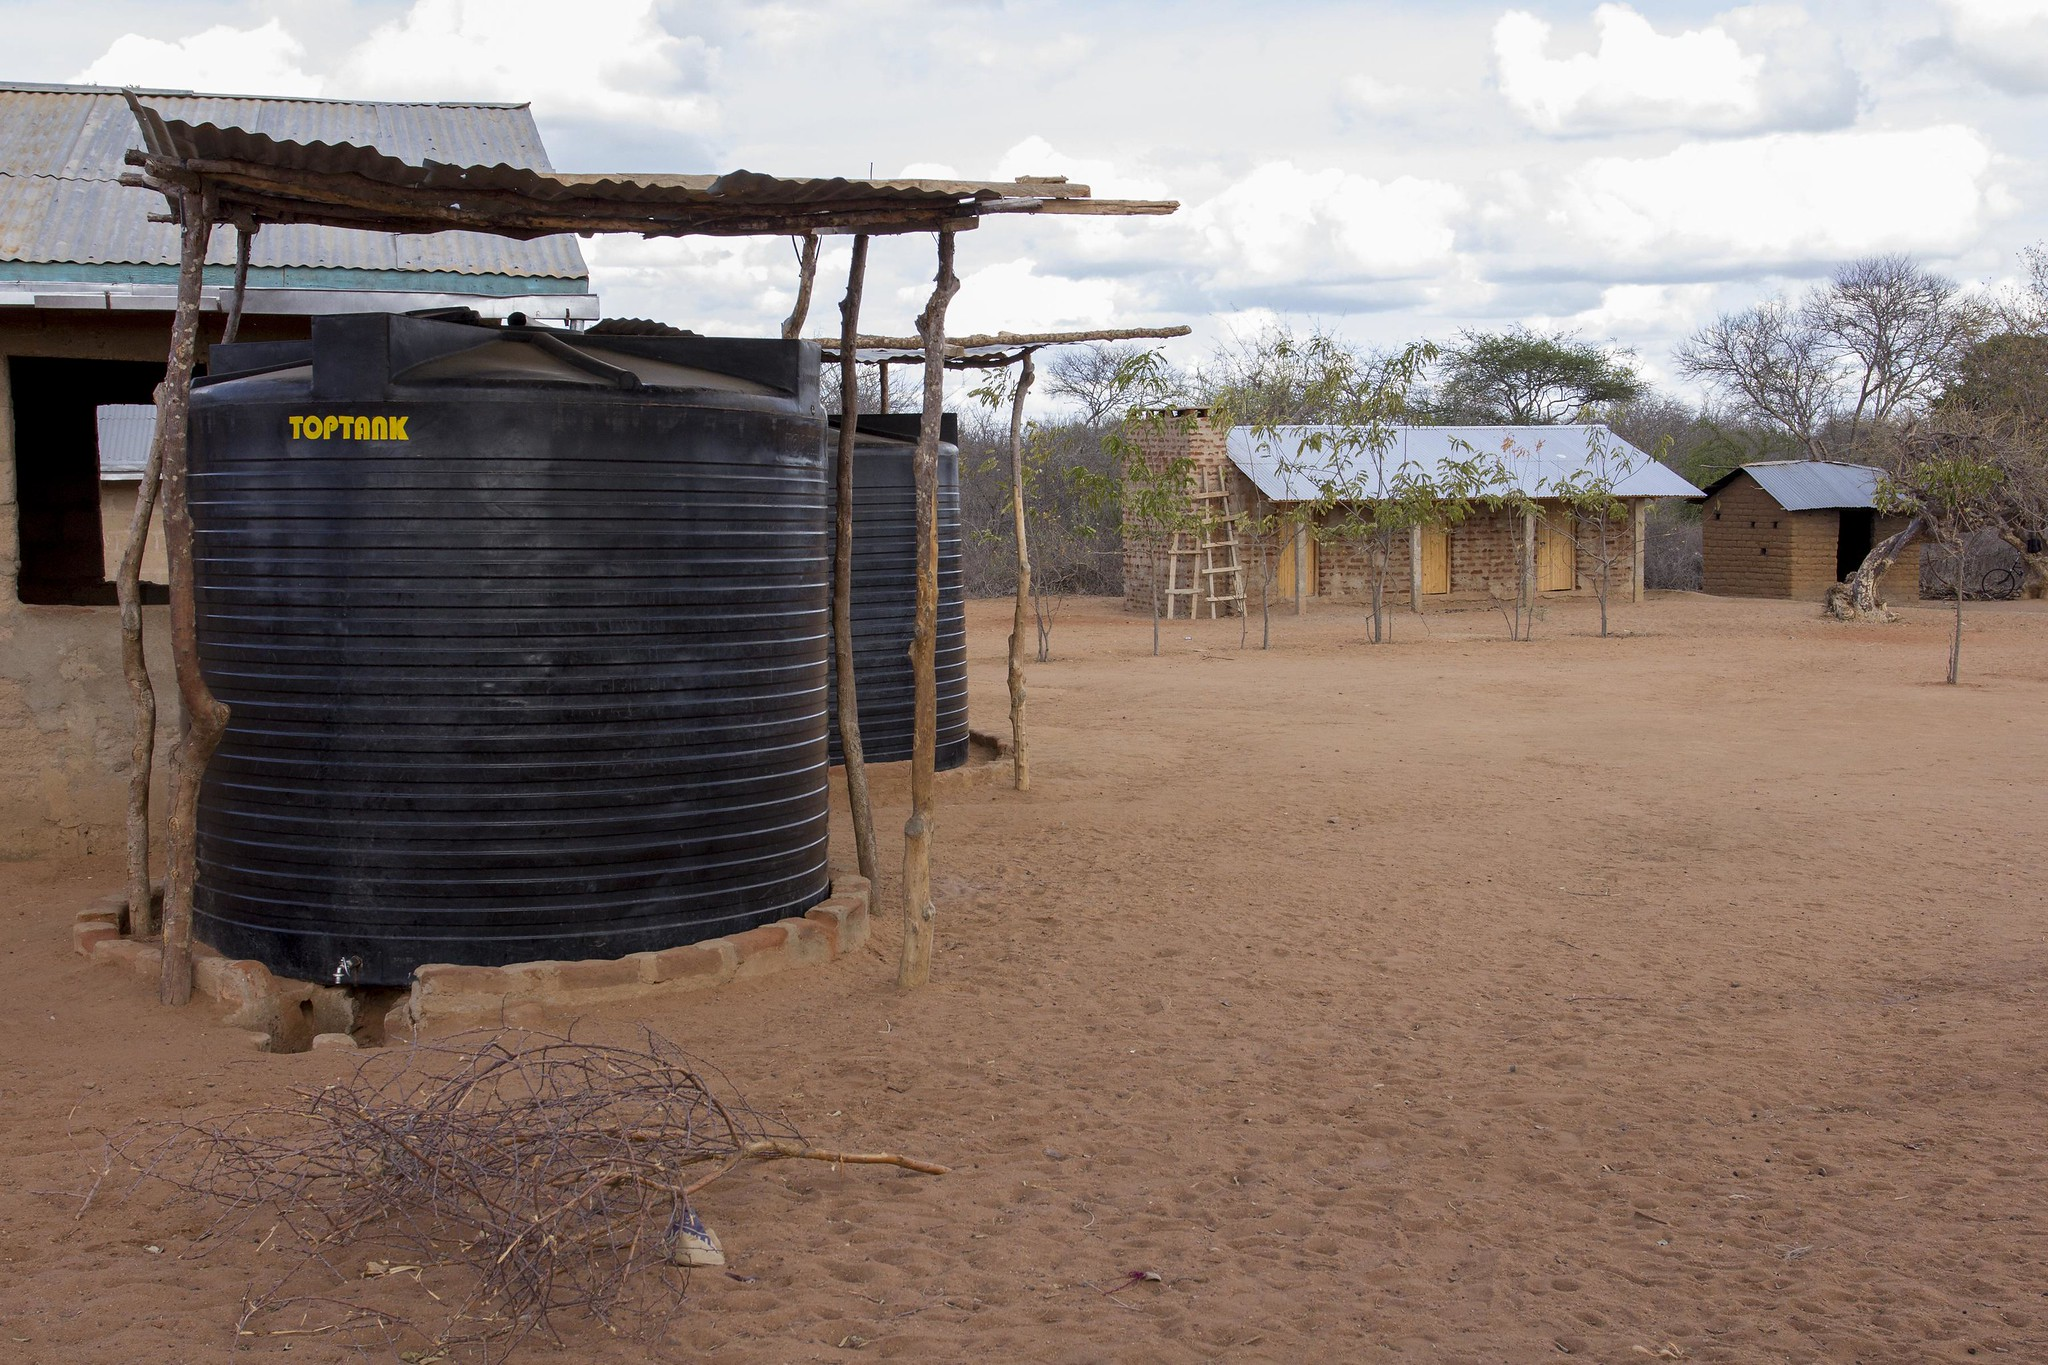
\includegraphics[keepaspectratio,height=0.9\paperheight]{photos/Kenya-cistern-Flore-de-Preneuf-2011-LARGE.jpg}};
%		
%		\node [anchor=east,align=right] at (6,-2.25) {\Large{\textcolor{white}{Williams College ECON 379:}}};		
%		\node [anchor=east,align=right] at (6,-3) {\Large{\textcolor{white}{Program Evaluation for International Development}}};
%
%		\node [anchor=east] at (6,-3.8) {\textcolor{yellow}{\tiny{photo:  Flore de Preneuf / World Bank}}};
%		
%		\end{tikzpicture}
%\end{center}
%
%\end{frame}


%%%%%%%%%%%%%%%%%%%%%%%%%%%%%%%%%%%%%%%%%%%%%%%%%%%%%%%%%%%%%%%%%%%%%%%%%%
% COURSE Title slide - for version with NO white space for head
%%%%%%%%%%%%%%%%%%%%%%%%%%%%%%%%%%%%%%%%%%%%%%%%%%%%%%%%%%%%%%%%%%%%%%%%%%

\begin{frame}<beamer:0>[plain]


\begin{center}
	\begin{tikzpicture}
	
	\node [opacity=1] (bg) at (0,0)  {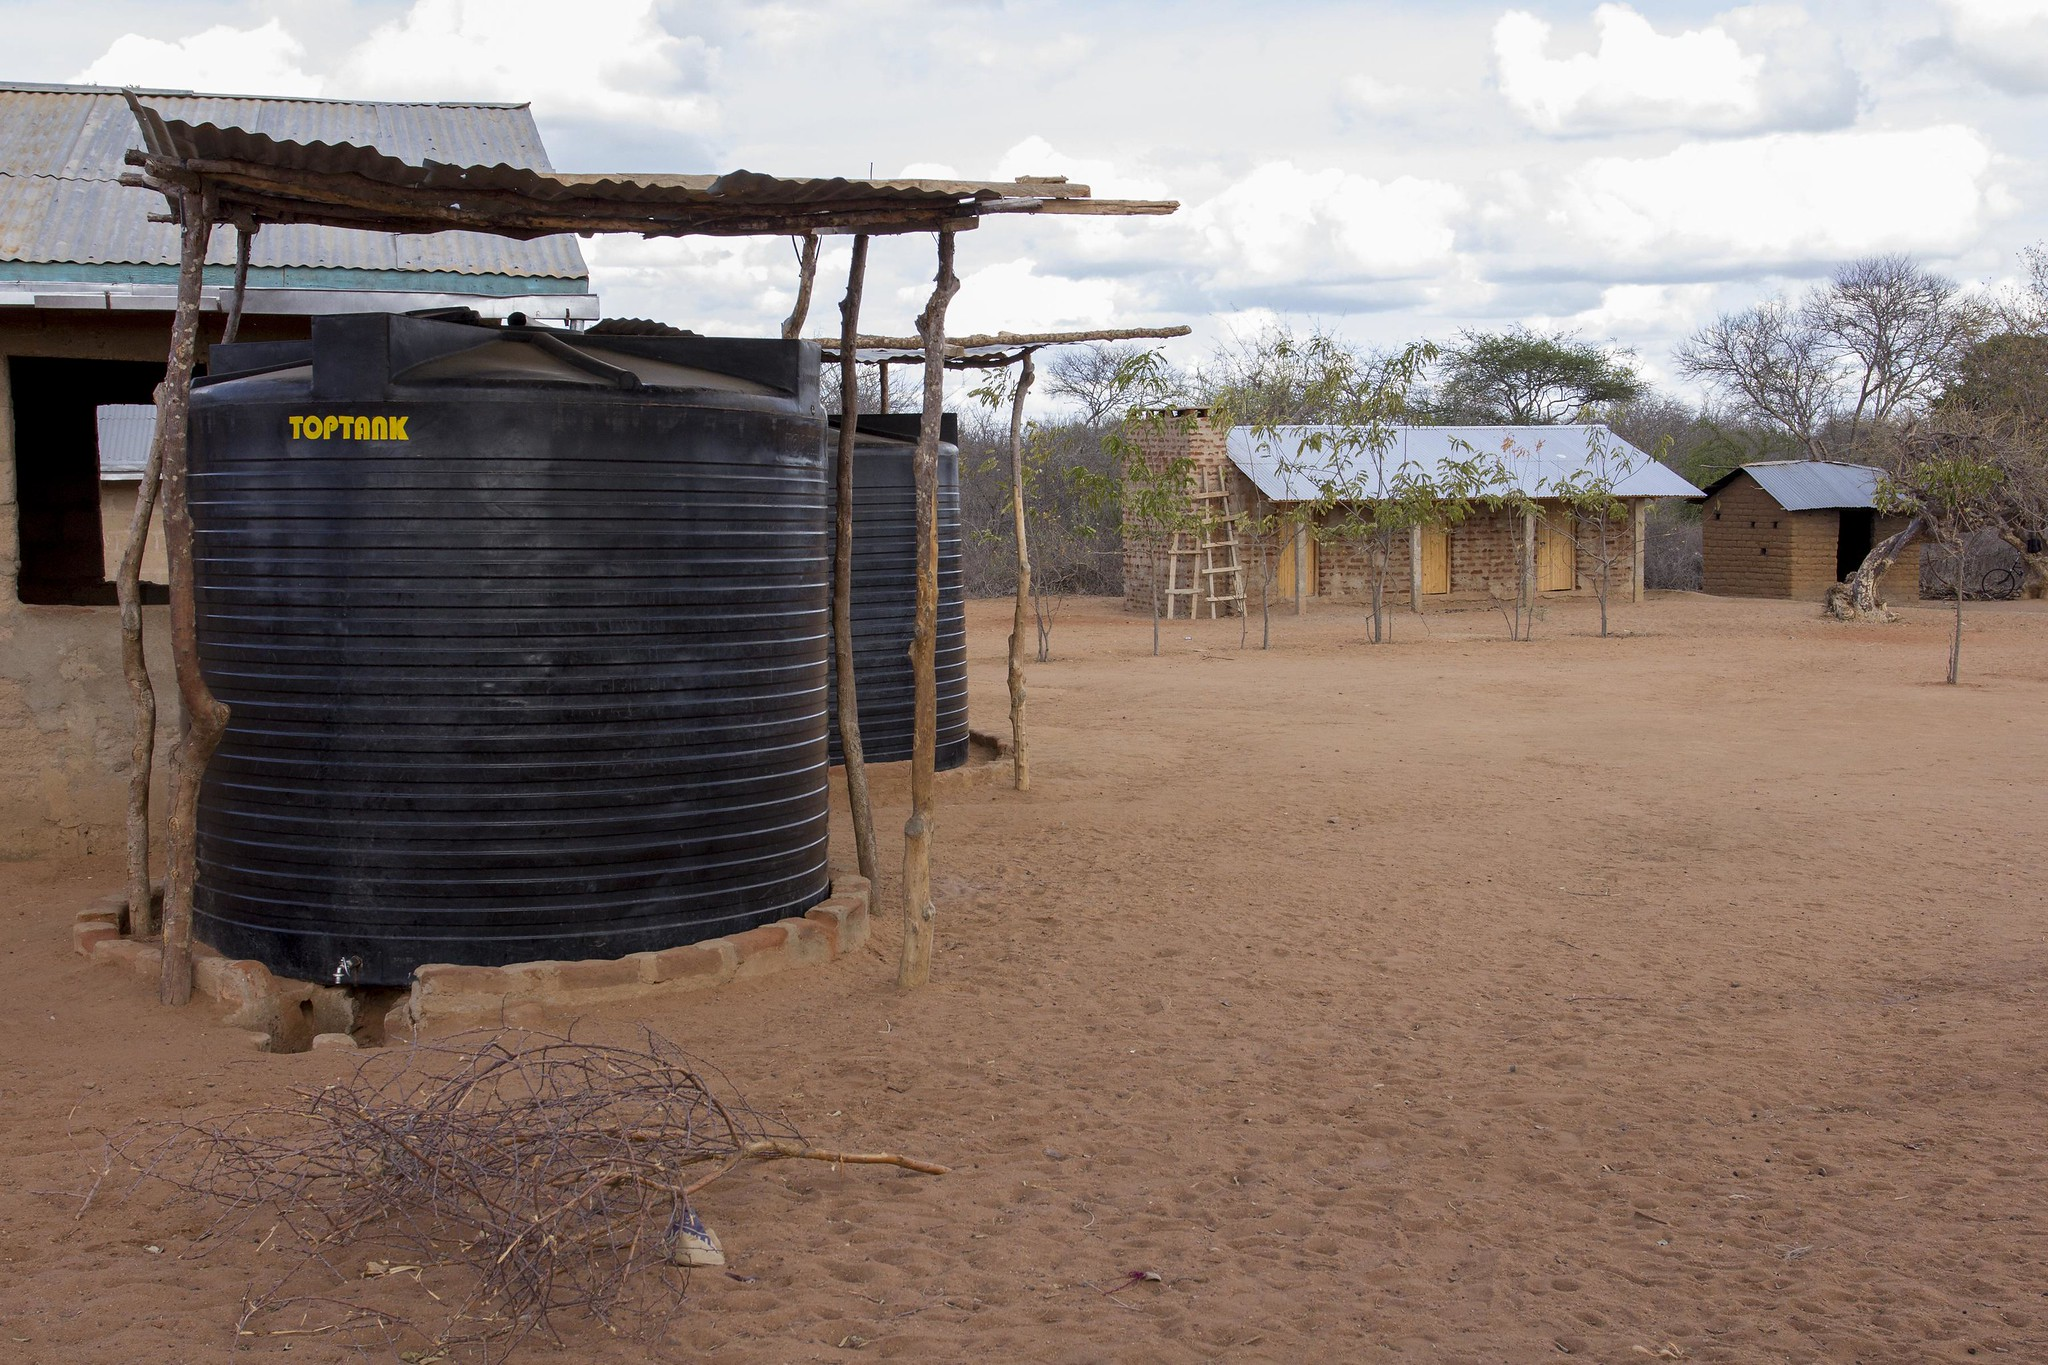
\includegraphics[keepaspectratio,width=10cm]{photos/Kenya-cistern-Flore-de-Preneuf-2011-LARGE.jpg}};
	
	\node [anchor=east,align=right,white,font=\large] at (5,-1.75) {Williams College ECON 379:};		
	\node [anchor=east,align=right,white,font=\large] at (5,-2.3255) {Program Evaluation for International Development};
	
	\node [anchor=east,yellow,font=\tiny] at (5,-3) {photo:  Flore de Preneuf / World Bank};
	
	\end{tikzpicture}
\end{center}

\end{frame}


%%%%%%%%%%%%%%%%%%%%%%%%%%%%%%%%%%%%%%%%%%%%%%%%%%%%%%%%%%%%%%%%%%%%%%%%%%
% LECTURE Title slide - version with white space for head
%%%%%%%%%%%%%%%%%%%%%%%%%%%%%%%%%%%%%%%%%%%%%%%%%%%%%%%%%%%%%%%%%%%%%%%%%%

%\begin{frame}[plain]
%
%\begin{center}
%	\begin{tikzpicture}
%	
%	\node [opacity=0.25] (bg)  {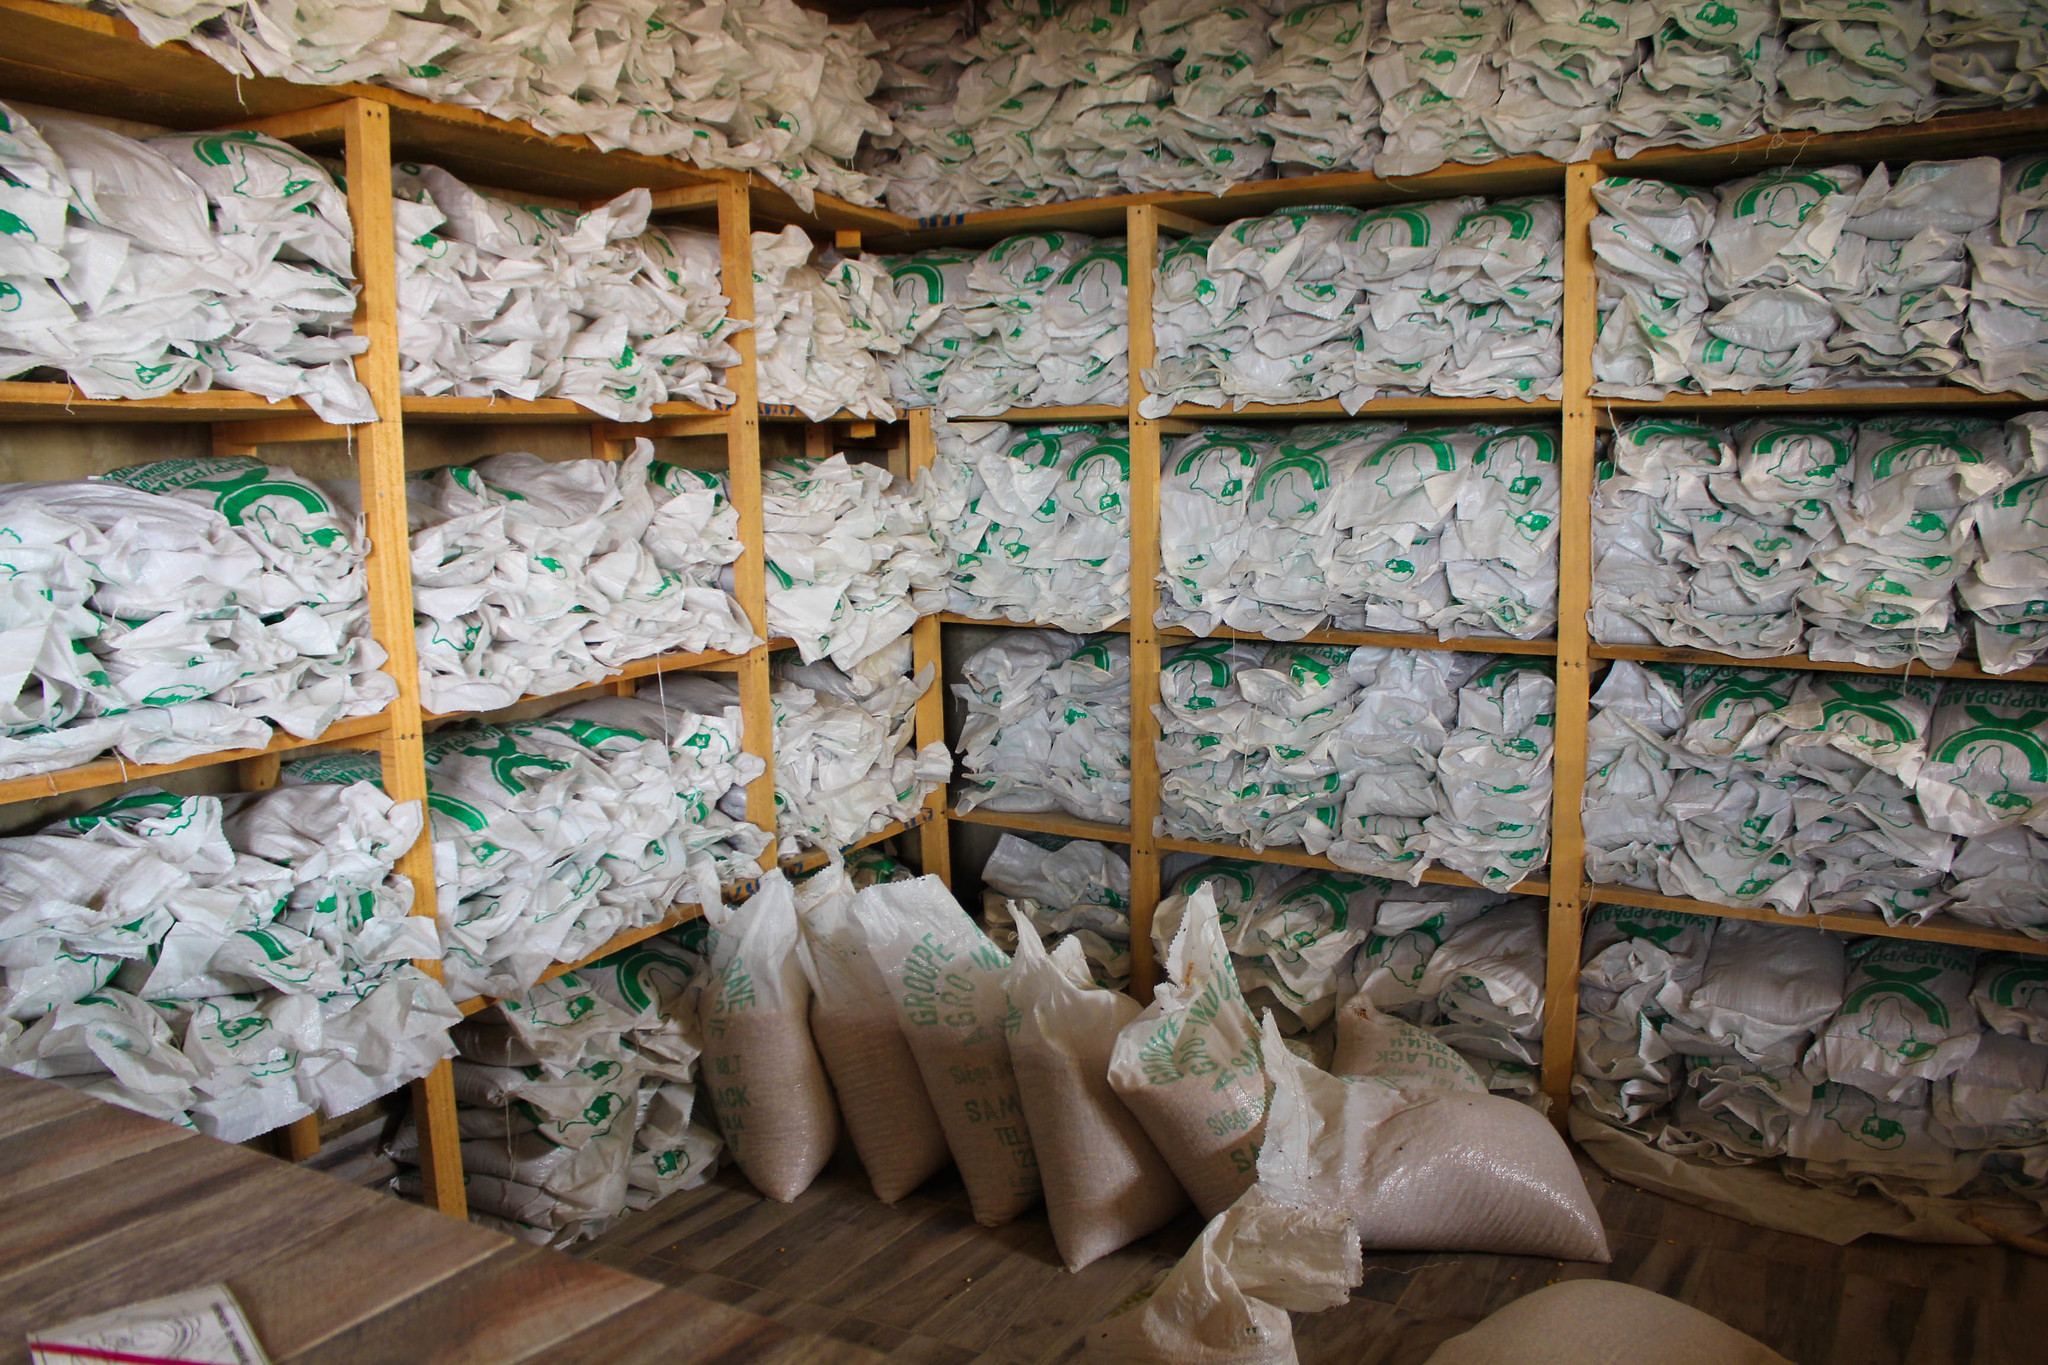
\includegraphics[keepaspectratio,height=0.9\paperheight]{photos/Senegal-WAAPP-seeds-Daniella-Van-Leggelo-Padilla-LARGE.jpg}};
%	
%	\node at (0,2.5) {\large{\textcolor{williams}{Williams College ECON 379:}}};		
%	\node at (0,1.5) {\large{\textcolor{williams}{Program Evaluation for International Development}}};
%	
%	\node at (0,-0.5) {\large{\textcolor{williams}{\textbf{Module 2: Selection Bias and the Experimental Ideal}}}};
%	
%	\node at (0,-2) {\large{\textcolor{williams}{Professor:  Pamela Jakiela}}};
%	
%	\node [anchor=east] at (6,-3.8) {\textcolor{yellow}{\tiny{photo:  Daniella Van Leggelo-Padilla / World Bank}}};
%	
%	\end{tikzpicture}
%\end{center}
%
%\end{frame}


%%%%%%%%%%%%%%%%%%%%%%%%%%%%%%%%%%%%%%%%%%%%%%%%%%%%%%%%%%%%%%%%%%%%%%%%%%
% LECTURE Title slide - version with NO white space for head
%%%%%%%%%%%%%%%%%%%%%%%%%%%%%%%%%%%%%%%%%%%%%%%%%%%%%%%%%%%%%%%%%%%%%%%%%%

\begin{frame}[plain]

\begin{center}
	\begin{tikzpicture}
	
	\node [opacity=0.25] (bg)  {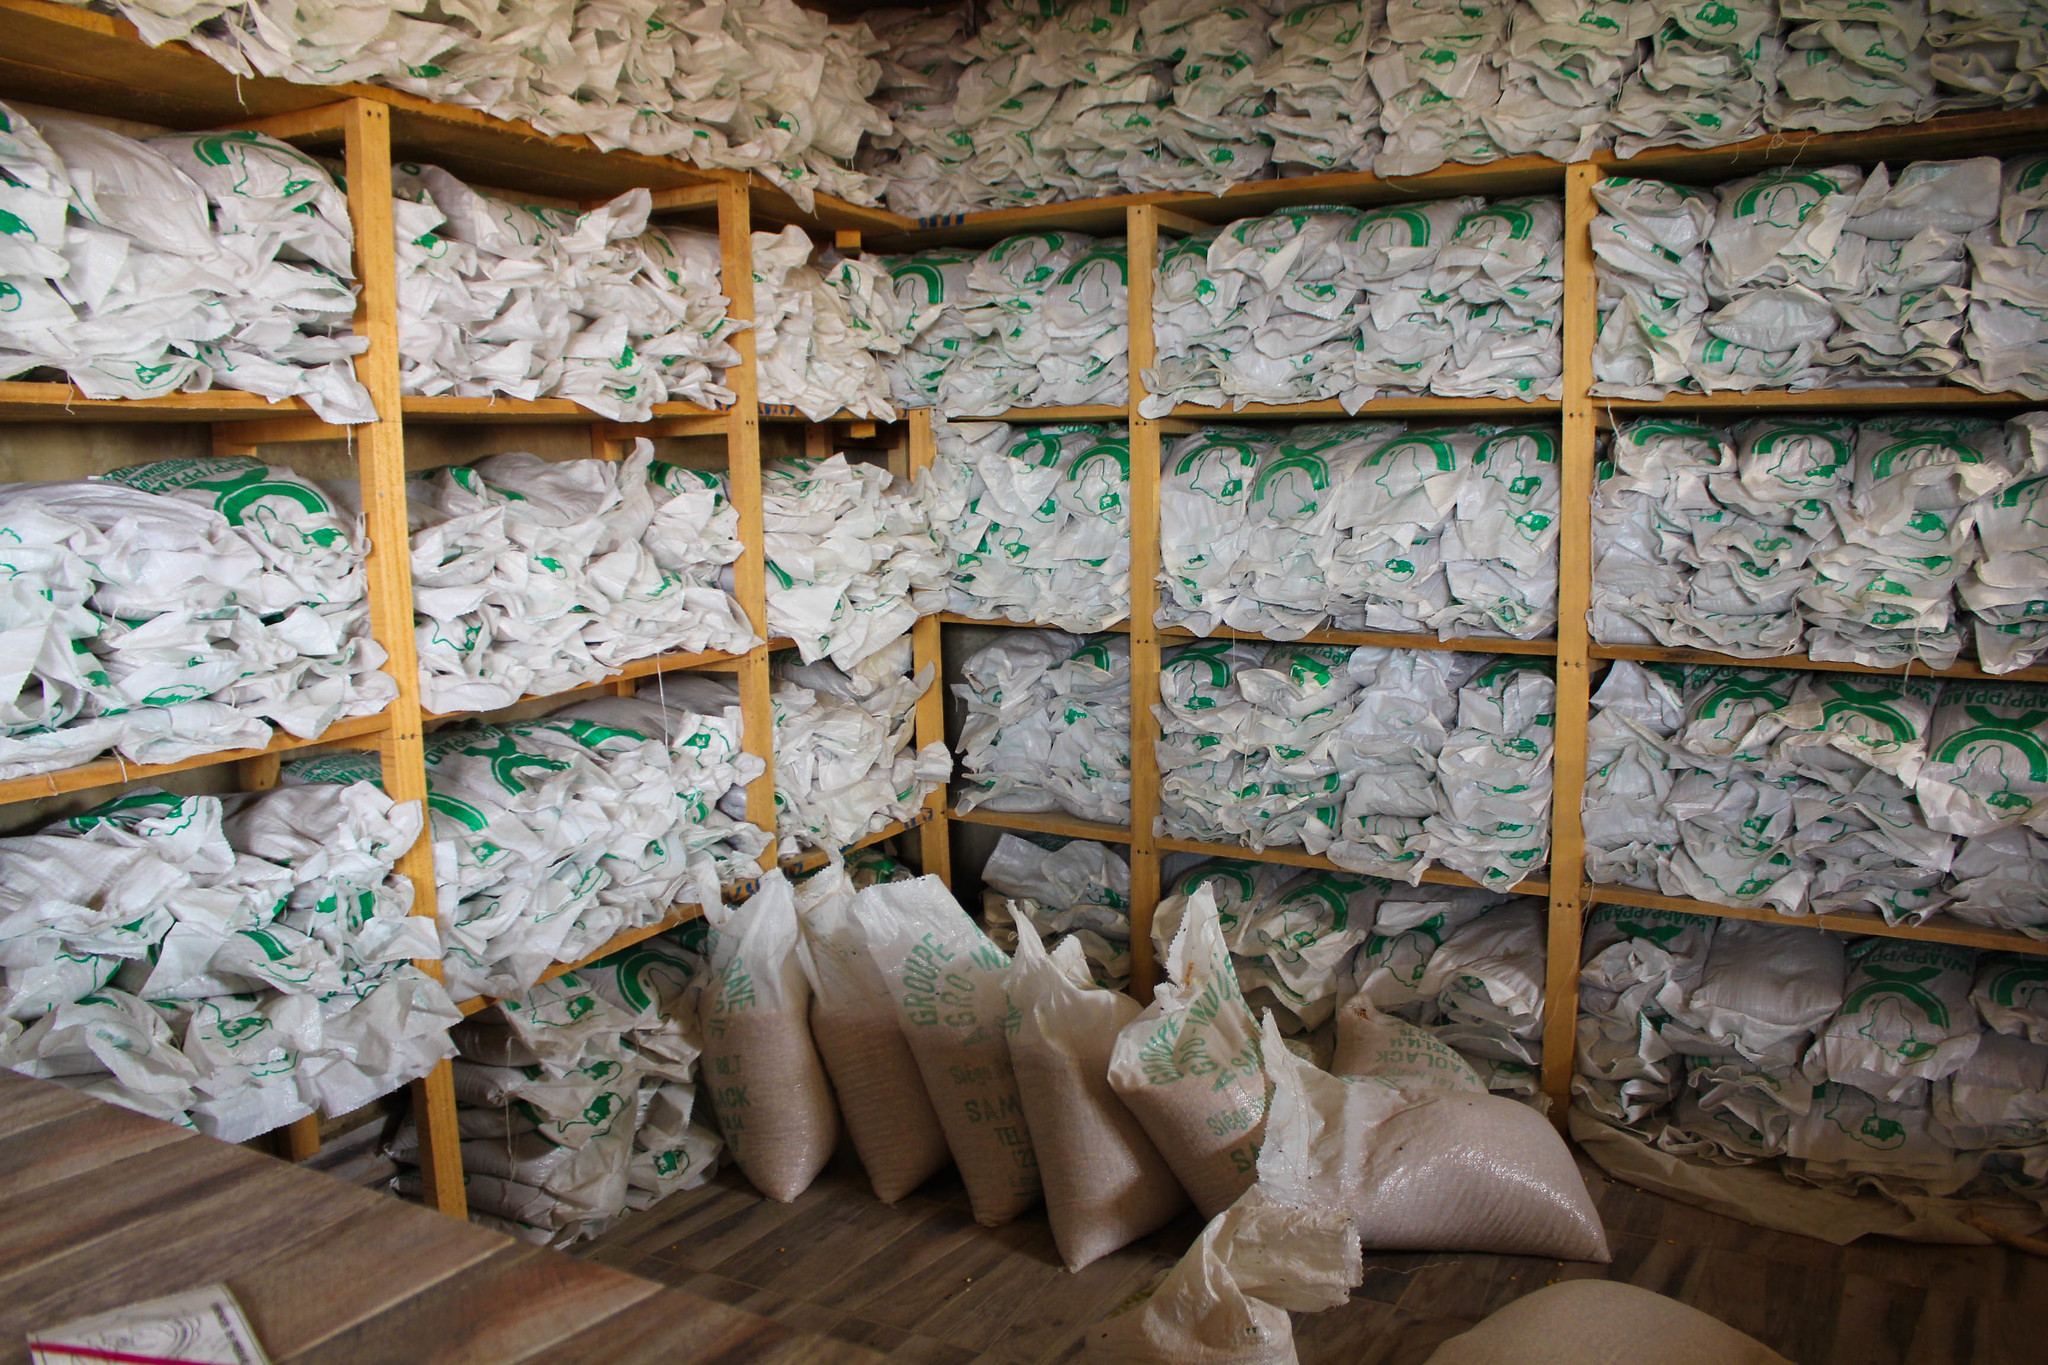
\includegraphics[keepaspectratio,width=10cm]{photos/Senegal-WAAPP-seeds-Daniella-Van-Leggelo-Padilla-LARGE.jpg}};
	
	\node at (0,2.5) {\large{\textcolor{williams}{Williams College ECON 379:}}};		
	\node at (0,1.5) {\large{\textcolor{williams}{Program Evaluation for International Development}}};
	
	%\node at (0,-0.5) {\large{\textcolor{williams}{\textbf{Module 2: Selection Bias and the Experimental Ideal}}}};
	\node at (0,-0.5) {\large{\textcolor{williams}{\textbf{Module 2: Selection Bias}}}};
	
	\node at (0,-2) {\large{\textcolor{williams}{Professor:  Pamela Jakiela}}};
	
	\node [anchor=east] at (5,-3) {\textcolor{yellow}{\tiny{photo:  Daniella Van Leggelo-Padilla / World Bank}}};
	
	\end{tikzpicture}
\end{center}

\end{frame}



%%%%%%%%%%%%%%%%%%%%%%%%%%%%%%%%%%%%%%%%%%%%%%%%%%%%%%%%%%%%%%%%%%%%%%%%%%%

%\begin{frame}<handout:0>[bg,plain]
\begin{frame}[plain]

%\only<beamer>{\begin{adjustwidth}{0cm}{-4cm}}

\begin{center}
	
	%\Large{\textcolor{white}{Budget Sets and Budget Lines}}
	\Large{\textcolor{williams}{Potential Outcomes}}
	
\end{center}

%\only<beamer>{\end{adjustwidth}}
\end{frame}



%%%%%%%%%%%%%%%%%%%%%%%%%%%%%%%%%%%%%%%%%%%%%%%%%%%%%%%%%%%%%%%%%%%%%

\begin{frame}{Do Hospitals Make People Healthier?}

\medskip

Your health status is:  excellent, very good, good, fair, or poor?

\medskip
\medskip
\begin{center}
	\begin{tabular}{lccc}
		& \textbf{Hospital}    & \textbf{No Hospital}     & \textbf{Difference} \\ [0.4ex]
		\hline
		& & & \\ [-2ex]
		Health status   & 3.21                      & 3.93                          & $-0.72^{\ast \ast \ast}$ \\ [0.6ex]
		& (0.014)                   & (0.003)                       & \\ [0.6ex]
		Observations    & 7,774                     & 90,049                        & \\ [0.6ex]
		\hline
	\end{tabular}
\end{center}

\medskip
\medskip
A comparison of means suggests hospitals make people worse off:  those who had a hospital stay in the last 6 months are, on average, less healthy than those that were not admitted to the hospital
 
\pause
\medskip
\begin{itemize}
	
	\item What's wrong with this picture?
	
\end{itemize}

\end{frame}

\noindent
\HRule

\medskip
\noindent
Data from the 2005 National Health Interview Survey


%%%%%%%%%%%%%%%%%%%%%%%%%%%%%%%%%%%%%%%%%%%%%%%%%%%%%%%%%%%%%%%%%%%%%

\begin{frame}{Potential Outcomes}

\medskip
We are interested in the relationship between ``\textbf{treatment}'' and 
some outcome that may be impacted by the treatment (eg.~health)

\pause
\medskip
\medskip
Outcome of interest:

\medskip
\begin{itemize}
	
	\item $Y = $ outcome we are interested in studying  (e.g.~health)
	
	\item $Y_i = $ value of outcome of interest \emph{for individual} $i$
	
\end{itemize}

\pause
\medskip
\medskip
For each individual, there are two \textbf{potential outcomes}:

\medskip
\begin{itemize}
	
	\item $Y_{0,i} = $ $i$'s outcome if she \textbf{doesn't} receive treatment
	
	\item $Y_{1,i} = $ $i$'s outcome if she \textbf{does} receive treatment
	
\end{itemize}

\end{frame}

%%%%%%%%%%%%%%%%%%%%%%%%%%%%%%%%%%%%%%%%%%%%%%%%%%%%%%%%%%%%%%%%%%%%%

\begin{frame}{Potential Outcomes:  Example}

\medskip

Alejandro has a broken leg.

\medskip
\begin{itemize}
	
	\item $Y_{0,a}$ = If he doesn't go to the hospital, his leg won't heal
	
	\item \textcolor{red}{$Y_{1,a}$ = If he goes to the hospital, his leg heals completely}
	
\end{itemize}

\pause
\medskip
\medskip
Benicio doesn't have any broken bones.  His health is fine.

\medskip
\begin{itemize}
	
	\item \textcolor{red}{$Y_{0,b}$ = If he doesn't go to the hospital, his health is still fine}
	
	\item $Y_{1,b}$ = If he goes to the hospital, his health is still fine
	
\end{itemize}

\end{frame}


%%%%%%%%%%%%%%%%%%%%%%%%%%%%%%%%%%%%%%%%%%%%%%%%%%%%%%%%%%%%%%%%%%%%%

\begin{frame}{Potential Outcomes:  Example}

\medskip
\begin{center}
\begin{tabular}{rcc}
 & \textbf{Yes Hospital} & \textbf{No Hospital} \\ [0.4ex] \hline
 & & \\ [-1.2ex]
Alejandro 	& \textcolor{red}{$Y_{1,a}$} 	& \textcolor{black}{$Y_{0,a}$} \\ [1.2ex] 
Benicio 	& \textcolor{black}{$Y_{1,b}$}						& \textcolor{red}{$Y_{0,b}$} \\ [0.8ex] \hline
	& \multicolumn{1}{p{1.6cm}}{$\ $} & \multicolumn{1}{p{1.6cm}}{$\ $} \\
\end{tabular}
\end{center}

\end{frame}


%%%%%%%%%%%%%%%%%%%%%%%%%%%%%%%%%%%%%%%%%%%%%%%%%%%%%%%%%%%%%%%%%%%%%

\begin{frame}<handout:0>{Potential Outcomes:  Example}

\medskip
\begin{center}
	\begin{tabular}{rcc}
		& \textbf{Yes Hospital} & \textbf{No Hospital} \\ [0.4ex] \hline
		& & \\ [-1.2ex]
		Alejandro 	& \textcolor{red}{$Y_{1,a}$} 	& \textcolor{white}{$Y_{0,a}$} \\ [1.2ex] 
		Benicio 	& \textcolor{white}{$Y_{1,b}$}						& \textcolor{red}{$Y_{0,b}$} \\ [0.8ex] \hline
		& \multicolumn{1}{p{1.6cm}}{$\ $} & \multicolumn{1}{p{1.6cm}}{$\ $} \\
	\end{tabular}
\end{center}

\end{frame}



%%%%%%%%%%%%%%%%%%%%%%%%%%%%%%%%%%%%%%%%%%%%%%%%%%%%%%%%%%%%%%%%%%%%%

\begin{frame}{The Fundamental Problem of Causal Inference}

\textbf{The fundamental problem of causal inference:}

\medskip

We never observe both potential outcomes for the same individual

\medskip
\begin{itemize}
	
	\item[$\Rightarrow$] Creates a missing data problem whenever we try to compare \textcolor{red}{treated} (i.e.~those who receive treatment) to \textcolor{red}{untreated} 
	
\end{itemize}

\pause
\medskip
\medskip
For any individual, we can only observe one potential outcome:
\begin{equation*}
Y_i =
\begin{cases}Y_{0,i} & \textsf{if } D_i = 0 \\
Y_{1,i} & \textsf{if } D_i = 1 \\
\end{cases} 
\end{equation*}
where \textcolor{red}{$D_i$ is a treatment indicator (equal to 1 if $i$ was treated)}

\end{frame}


%%%%%%%%%%%%%%%%%%%%%%%%%%%%%%%%%%%%%%%%%%%%%%%%%%%%%%%%%%%%%%%%%%%%%

\begin{frame}{Defining the Causal Effect of Treatment}

\medskip
\fbox{\textcolor{red}{The causal impact of the program on $i$ is:  $Y_{1,i} - Y_{0,i} $}}

\pause
\medskip
\begin{itemize}
	
	\item
	Each individual either participates in the program or not
	
\end{itemize}

\pause
\medskip
\medskip
We only observe $i$'s actual outcome:
\begin{flalign*}
Y_i = \textcolor{black}{Y_{0,i}} \ \textcolor{black}{+} \ \textcolor{black}{\underbrace{ \left( \textcolor{black}{Y_{1,i}} - Y_{0,i} \right) }_{impact}  D_i} &&
\end{flalign*}

Example:  Alejandro goes to the hospital, Benicio does not

\end{frame}


%%%%%%%%%%%%%%%%%%%%%%%%%%%%%%%%%%%%%%%%%%%%%%%%%%%%%%%%%%%%%%%%%%%%%

\begin{frame}<handout:0>{Defining the Causal Effect of Treatment}

\medskip
\fbox{\textcolor{red}{The causal impact of the program on $i$ is:  $Y_{1,i} - Y_{0,i} $}}

\medskip
\begin{itemize}
	
	\item
	Each individual either participates in the program or not
	
\end{itemize}

\medskip
\medskip
We only observe $i$'s actual outcome:
\begin{flalign*}
Y_i = \textcolor{red}{Y_{0,i}} \ \textcolor{gray!50}{+} \ \textcolor{gray!50}{\underbrace{ \left( \textcolor{gray!50}{Y_{1,i}} - Y_{0,i} \right) }_{impact}  D_i} &&
\end{flalign*}

Example:  Alejandro goes to the hospital, Benicio does not

\end{frame}


%%%%%%%%%%%%%%%%%%%%%%%%%%%%%%%%%%%%%%%%%%%%%%%%%%%%%%%%%%%%%%%%%%%%%

\begin{frame}<handout:0>{Defining the Causal Effect of Treatment}

\medskip
\fbox{\textcolor{red}{The causal impact of the program on $i$ is:  $Y_{1,i} - Y_{0,i} $}}

\medskip
\begin{itemize}
	
	\item
	Each individual either participates in the program or not
	
\end{itemize}

\medskip
\medskip
We only observe $i$'s actual outcome:
\begin{flalign*}
Y_i = \textcolor{gray!50}{Y_{0,i}} \ \textcolor{gray!50}{+} \ \textcolor{gray!50}{\underbrace{ \left( \textcolor{red}{Y_{1,i}} - Y_{0,i} \right) }_{impact}  D_i} &&
\end{flalign*}

Example:  Alejandro goes to the hospital, Benicio does not

\end{frame}



%%%%%%%%%%%%%%%%%%%%%%%%%%%%%%%%%%%%%%%%%%%%%%%%%%%%%%%%%%%%%%%%%%%%%

\begin{frame}{Establishing Causality}

\medskip
In an ideal world (research-wise), we could clone each treated individual and observe the impacts of treatment on outcomes 

\begin{center}
	\begin{tabular}{ccc}
		
\includegraphics[height=2.2cm]{img/lisa1.png} & vs. & 
\includegraphics[height=2.2cm]{img/lisa-book.jpg}
	\end{tabular}
\end{center}

\medskip
What is the impact of giving Lisa a textbook on her test score?

\medskip
\begin{itemize}
	
	\item
	Impact = Lisa's score with a book - Lisa's score without a book
	
\end{itemize}

\pause
\medskip
In the real world, we either observe Lisa with a textbook or without

\medskip
\begin{itemize}
	
	\item
	Can't observe the \textbf{counterfactual} (other potential outcome)
	
\end{itemize}

\end{frame}


%%%%%%%%%%%%%%%%%%%%%%%%%%%%%%%%%%%%%%%%%%%%%%%%%%%%%%%%%%%%%%%%%%%%%

\begin{frame}{Establishing Causality}

\medskip
To measure the causal impact of giving Lisa a book on her test score, 
we need to find a similar child that did not receive a book

\begin{center}
	\begin{tabular}{ccc}
		
\includegraphics[height=2.4cm]{img/bart.png} & vs. & 
\includegraphics[height=2.2cm]{img/lisa-book.jpg}
	\end{tabular}
\end{center}

Our estimate of the impact of the book is then the difference in test scores between the \textbf{treatment group} and the \textbf{comparison group}

\medskip
\begin{itemize}
	
	\item
	Impact = Lisa's score w/ book - Bart's score w/o book
	
\end{itemize}

\pause
\medskip
As this example illustrates, finding a good comparison group is hard

\medskip
\begin{itemize}
	
	\item
	In applied micro, your research design \textbf{is} your counterfactual
	
\end{itemize}

\end{frame}


%%%%%%%%%%%%%%%%%%%%%%%%%%%%%%%%%%%%%%%%%%%%%%%%%%%%%%%%%%%%%%%%%%%%%

\begin{frame}{Average Causal Effects}

\medskip
What we actually want to know is the \textbf{average causal effect}, \\
which is not what we get from a difference in means comparison
\medskip
\begin{small}
	\begin{align*}
	&\textbf{Difference in group means} \\
	& \\
	& \ \ \ \ \ \ \ \  = \textsf{average causal effect of program on participants} + \textsf{selection bias}\\
	\end{align*}
\end{small}

\vspace{-0.5cm}

\pause
Even in a large sample:

\medskip
\begin{itemize}
	
	\item People will choose to participate in a program when they expect it to make them better off (i.e.~when $Y_{1,i} - Y_{0,i} > 0$)
	
	\item People who choose (or get) to participate maybe different than those who choose not to$\ldots$ \textcolor{red}{even in the absence of the program}
	
\end{itemize}

\end{frame}


%%%%%%%%%%%%%%%%%%%%%%%%%%%%%%%%%%%%%%%%%%%%%%%%%%%%%%%%%%%%%%%%%%%%%%%

\begin{frame}{Selection Bias:  Example}

\begin{center}
	\begin{tikzpicture}
	
	% blank canvas
	\only<handout>{\fill[fill=white,draw=white,ultra thin]
	(0,0) -- (11,0) -- (11,6) -- (0,6) -- cycle;}
	\only<beamer>{\fill[fill=white,draw=white,ultra thin]
	(0,0) -- (14,0) -- (14,6) -- (0,6) -- cycle;}
	\only<beamer>{\draw[draw=oiblue!60,fill=oiblue!10,opacity=0.5] (11,1) rectangle (14,5);}
	%\draw[step=1.0,gray!20,thin] (0,0) grid (11,6);
	
	%\pgfmathsetmacro\xshift{0.5cm};
	%\pgfmathsetmacro\yshift{5.5cm};
	\pgfmathsetmacro\mycolor{"gray"};
	
	\draw[\mycolor,thick] (1.25,4.875) -- (4.5,4.875) (1.25,1.875) -- (4.5,1.875);
	
	\node[\mycolor,anchor=west,align=left] at (1.25,4.5) {Alice};
	\node[\mycolor,anchor=west,align=left] at (1.25,3.75) {Betty};
	\node[\mycolor,anchor=west,align=left] at (1.25,3) {Carol};
	\node[\mycolor,anchor=west,align=left] at (1.25,2.25) {Diana};
	
	\node[\mycolor,anchor=south] at (3,5) {$Y_{1,i}$};
	\node[\mycolor] at (3,4.5) {6};
	\node[\mycolor] at (3,3.75) {7};
	\node[\mycolor] at (3,3) {3};
	\node[\mycolor] at (3,2.25) {4};
	
	\node[\mycolor,anchor=south] at (4,5) {$Y_{0,i}$};
	\node[\mycolor] at (4,4.5) {4};
	\node[\mycolor] at (4,3.75) {5};
	\node[\mycolor] at (4,3) {1};
	\node[\mycolor] at (4,2.25) {2};
	
	\end{tikzpicture}
\end{center}
\end{frame}


%%%%%%%%%%%%%%%%%%%%%%%%%%%%%%%%%%%%%%%%%%%%%%%%%%%%%%%%%%%%%%%%%%%%%%%

\begin{frame}<handout:0>{Selection Bias:  Example}

\begin{center}
	\begin{tikzpicture}
	
	% blank canvas
	\only<handout>{\fill[fill=white,draw=white,ultra thin]
		(0,0) -- (11,0) -- (11,6) -- (0,6) -- cycle;}
	\only<beamer>{\fill[fill=white,draw=white,ultra thin]
		(0,0) -- (14,0) -- (14,6) -- (0,6) -- cycle;}
	\only<beamer>{\draw[draw=oiblue!60,fill=oiblue!10,opacity=0.5] (11,1) rectangle (14,5);}
	%\draw[step=1.0,gray!20,thin] (0,0) grid (11,6);
	
	%\pgfmathsetmacro\xshift{0.5cm};
	%\pgfmathsetmacro\yshift{5.5cm};
	\pgfmathsetmacro\mycolor{"gray"};

	% table of potential outcomes
		
	\draw[\mycolor,thick] (1.25,4.875) -- (4.5,4.875) (1.25,1.875) -- (4.5,1.875);
	
	\node[\mycolor,anchor=west,align=left] at (1.25,4.5) {Alice};
	\node[\mycolor,anchor=west,align=left] at (1.25,3.75) {Betty};
	\node[\mycolor,anchor=west,align=left] at (1.25,3) {Carol};
	\node[\mycolor,anchor=west,align=left] at (1.25,2.25) {Diana};
	
	\node[\mycolor,anchor=south] at (3,5) {$Y_{1,i}$};
	\node[\mycolor] at (3,4.5) {6};
	\node[\mycolor] at (3,3.75) {7};
	\node[\mycolor] at (3,3) {3};
	\node[\mycolor] at (3,2.25) {4};
	
	\node[\mycolor,anchor=south] at (4,5) {$Y_{0,i}$};
	\node[\mycolor] at (4,4.5) {4};
	\node[\mycolor] at (4,3.75) {5};
	\node[\mycolor] at (4,3) {1};
	\node[\mycolor] at (4,2.25) {2};
	
	% highlight outcomes with treatment
	
	\draw[oiverm,thick] (2.625,1.75) -- (2.625,5.75) -- (3.375,5.75) -- (3.375,1.75) -- cycle;
	\node[oiverm] (lbl1) at (8,4.75) {outcomes with treatment};
	\draw[oiverm,->,thick] (lbl1.west) -- (3.5,4);
	
	\end{tikzpicture}
\end{center}
\end{frame}


%%%%%%%%%%%%%%%%%%%%%%%%%%%%%%%%%%%%%%%%%%%%%%%%%%%%%%%%%%%%%%%%%%%%%%%

\begin{frame}<handout:0>{Selection Bias:  Example}

\begin{center}
	\begin{tikzpicture}
	
	% blank canvas
	\only<handout>{\fill[fill=white,draw=white,ultra thin]
		(0,0) -- (11,0) -- (11,6) -- (0,6) -- cycle;}
	\only<beamer>{\fill[fill=white,draw=white,ultra thin]
		(0,0) -- (14,0) -- (14,6) -- (0,6) -- cycle;}
	\only<beamer>{\draw[draw=oiblue!60,fill=oiblue!10,opacity=0.5] (11,1) rectangle (14,5);}
	%\draw[step=1.0,gray!20,thin] (0,0) grid (11,6);
	
	%\pgfmathsetmacro\xshift{0.5cm};
	%\pgfmathsetmacro\yshift{5.5cm};
	\pgfmathsetmacro\mycolor{"gray"};
	
	% table of potential outcomes
	
	\draw[\mycolor,thick] (1.25,4.875) -- (4.5,4.875) (1.25,1.875) -- (4.5,1.875);
	
	\node[\mycolor,anchor=west,align=left] at (1.25,4.5) {Alice};
	\node[\mycolor,anchor=west,align=left] at (1.25,3.75) {Betty};
	\node[\mycolor,anchor=west,align=left] at (1.25,3) {Carol};
	\node[\mycolor,anchor=west,align=left] at (1.25,2.25) {Diana};
	
	\node[\mycolor,anchor=south] at (3,5) {$Y_{1,i}$};
	\node[\mycolor] at (3,4.5) {6};
	\node[\mycolor] at (3,3.75) {7};
	\node[\mycolor] at (3,3) {3};
	\node[\mycolor] at (3,2.25) {4};
	
	\node[\mycolor,anchor=south] at (4,5) {$Y_{0,i}$};
	\node[\mycolor] at (4,4.5) {4};
	\node[\mycolor] at (4,3.75) {5};
	\node[\mycolor] at (4,3) {1};
	\node[\mycolor] at (4,2.25) {2};
	
	% highlight outcomes with treatment
	
	%\draw[gray!20,thick] (2.625,1.75) -- (2.625,5.75) -- (3.375,5.75) -- (3.375,1.75) -- cycle;
	%\node[gray!20] (lbl1) at (8,4.75) {outcomes with treatment};
	%\draw[gray!20,->,thick] (lbl1.west) -- (3.5,4);
	
	% highlight outcomes without treatment

	\draw[oiblue,thick] (3.625,1.75) -- (3.625,5.75) -- (4.375,5.75) -- (4.375,1.75) -- cycle;
	\node[oiblue] (lbl2) at (8,4) {outcomes without treatment};
	\draw[oiblue,->,thick] (lbl2.west) -- (4.5,3.5);
	
	\end{tikzpicture}
\end{center}
\end{frame}



%%%%%%%%%%%%%%%%%%%%%%%%%%%%%%%%%%%%%%%%%%%%%%%%%%%%%%%%%%%%%%%%%%%%%%%

\begin{frame}<handout:0>{Selection Bias:  Example}

\begin{center}
	\begin{tikzpicture}
	
	% blank canvas
	\only<handout>{\fill[fill=white,draw=white,ultra thin]
		(0,0) -- (11,0) -- (11,6) -- (0,6) -- cycle;}
	\only<beamer>{\fill[fill=white,draw=white,ultra thin]
		(0,0) -- (14,0) -- (14,6) -- (0,6) -- cycle;}
	\only<beamer>{\draw[draw=oiblue!60,fill=oiblue!10,opacity=0.5] (11,1) rectangle (14,5);}
	%\draw[step=1.0,gray!20,thin] (0,0) grid (11,6);
	
	%\pgfmathsetmacro\xshift{0.5cm};
	%\pgfmathsetmacro\yshift{5.5cm};
	\pgfmathsetmacro\mycolor{"gray"};
	
	% table of potential outcomes
	
	\draw[\mycolor,thick] (1.25,4.875) -- (4.5,4.875) (1.25,1.875) -- (4.5,1.875);
	
	\node[\mycolor,anchor=west,align=left] at (1.25,4.5) {Alice};
	\node[\mycolor,anchor=west,align=left] at (1.25,3.75) {Betty};
	\node[\mycolor,anchor=west,align=left] at (1.25,3) {Carol};
	\node[\mycolor,anchor=west,align=left] at (1.25,2.25) {Diana};
	
	\node[\mycolor,anchor=south] at (3,5) {$Y_{1,i}$};
	\node[\mycolor] at (3,4.5) {6};
	\node[\mycolor] at (3,3.75) {7};
	\node[\mycolor] at (3,3) {3};
	\node[\mycolor] at (3,2.25) {4};
	
	\node[\mycolor,anchor=south] at (4,5) {$Y_{0,i}$};
	\node[\mycolor] at (4,4.5) {4};
	\node[\mycolor] at (4,3.75) {5};
	\node[\mycolor] at (4,3) {1};
	\node[\mycolor] at (4,2.25) {2};
	
	% causal effect
	\pgfmathsetmacro\mycolor{"red"};
	\node[\mycolor,anchor=south] (causal) at (7,3.375) {causal effect:  $Y_{1,i} - Y_{0,i}$};
	\draw[\mycolor] (causal.south west) -- (causal.south east) -- ([yshift=0.05cm]causal.north east) -- ([yshift=0.05cm]causal.north west) -- cycle;

	
	\end{tikzpicture}
\end{center}
\end{frame}


%%%%%%%%%%%%%%%%%%%%%%%%%%%%%%%%%%%%%%%%%%%%%%%%%%%%%%%%%%%%%%%%%%%%%%%

\begin{frame}<handout:0>{Selection Bias:  Example}

\begin{center}
	\begin{tikzpicture}
	
	% blank canvas
	\only<handout>{\fill[fill=white,draw=white,ultra thin]
		(0,0) -- (11,0) -- (11,6) -- (0,6) -- cycle;}
	\only<beamer>{\fill[fill=white,draw=white,ultra thin]
		(0,0) -- (14,0) -- (14,6) -- (0,6) -- cycle;}
	\only<beamer>{\draw[draw=oiblue!60,fill=oiblue!10,opacity=0.5] (11,1) rectangle (14,5);}
	%\draw[step=1.0,gray!20,thin] (0,0) grid (11,6);
	
	%\pgfmathsetmacro\xshift{0.5cm};
	%\pgfmathsetmacro\yshift{5.5cm};
	\pgfmathsetmacro\mycolor{"gray"};
	
	% table of potential outcomes
	
	\draw[\mycolor,thick] (1.25,4.875) -- (4.5,4.875) (1.25,1.875) -- (4.5,1.875);
	
	\node[\mycolor,anchor=west,align=left] at (1.25,4.5) {Alice};
	\node[\mycolor,anchor=west,align=left] at (1.25,3.75) {Betty};
	\node[\mycolor,anchor=west,align=left] at (1.25,3) {Carol};
	\node[\mycolor,anchor=west,align=left] at (1.25,2.25) {Diana};
	
	\node[\mycolor,anchor=south] at (3,5) {$Y_{1,i}$};
	\node[\mycolor] at (3,4.5) {6};
	\node[\mycolor] at (3,3.75) {7};
	\node[\mycolor] at (3,3) {3};
	\node[\mycolor] at (3,2.25) {4};
	
	\node[\mycolor,anchor=south] at (4,5) {$Y_{0,i}$};
	\node[\mycolor] at (4,4.5) {4};
	\node[\mycolor] at (4,3.75) {5};
	\node[\mycolor] at (4,3) {1};
	\node[\mycolor] at (4,2.25) {2};
	
	% causal effect
	\pgfmathsetmacro\mycolor{"red"};
	%\node[\mycolor,anchor=south] at (7,5) {causal effect:  $Y_{1,i} - Y_{0,i}$};
	%\draw[\mycolor,thick] (5,4.875) -- (9,4.875) (5,1.875) -- (9,1.875);
	\node[\mycolor] at (3.5,4.5) {$-$};
	\node[\mycolor] at (3.5,3.75) {$-$};
	\node[\mycolor] at (3.5,3) {$-$};
	\node[\mycolor] at (3.5,2.25) {$-$};
	\node[\mycolor] at (4.5,4.5) {$=$};
	\node[\mycolor] at (4.5,3.75) {$=$};
	\node[\mycolor] at (4.5,3) {$=$};
	\node[\mycolor] at (4.5,2.25) {$=$};
	\node[\mycolor] at (5,4.5) {2};
	\node[\mycolor] at (5,3.75) {2};
	\node[\mycolor] at (5,3) {2};
	\node[\mycolor] at (5,2.25) {2};
	\draw [\mycolor,decorate,decoration={brace,amplitude=10pt},xshift=-4pt,yshift=0pt] 	(5.5,4.625) -- (5.5,2.125) node [\mycolor,anchor=west,align=left,midway,xshift=0.375cm,yshift=0.05cm] 	{$Y_{1,i} - Y_{0,i} = 2$ for all $i$};	
	
	\end{tikzpicture}
\end{center}
\end{frame}



%%%%%%%%%%%%%%%%%%%%%%%%%%%%%%%%%%%%%%%%%%%%%%%%%%%%%%%%%%%%%%%%%%%%%%%

\begin{frame}{Selection Bias:  Example}

\begin{center}
	\begin{tikzpicture}
	
	% blank canvas
	\only<handout>{\fill[fill=white,draw=white,ultra thin]
		(0,0) -- (11,0) -- (11,6) -- (0,6) -- cycle;}
	\only<beamer>{\fill[fill=white,draw=white,ultra thin]
		(0,0) -- (14,0) -- (14,6) -- (0,6) -- cycle;}
	\only<beamer>{\draw[draw=oiblue!60,fill=oiblue!10,opacity=0.5] (11,1) rectangle (14,5);}
	%\draw[step=1.0,gray!20,thin] (0,0) grid (11,6);
	
	%\pgfmathsetmacro\xshift{0.5cm};
	%\pgfmathsetmacro\yshift{5.5cm};
	\pgfmathsetmacro\mycolor{"gray"};
	
	% table of potential outcomes
	
	\draw[\mycolor,thick] (1.25,4.875) -- (4.5,4.875) (1.25,1.875) -- (4.5,1.875);
	
	\node[\mycolor,anchor=west,align=left] at (1.25,4.5) {Alice};
	\node[\mycolor,anchor=west,align=left] at (1.25,3.75) {Betty};
	\node[\mycolor,anchor=west,align=left] at (1.25,3) {Carol};
	\node[\mycolor,anchor=west,align=left] at (1.25,2.25) {Diana};
	
	\node[\mycolor,anchor=south] at (3,5) {$Y_{1,i}$};
	\node[\mycolor] at (3,4.5) {6};
	\node[\mycolor] at (3,3.75) {7};
	\node[\mycolor] at (3,3) {3};
	\node[\mycolor] at (3,2.25) {4};
	
	\node[\mycolor,anchor=south] at (4,5) {$Y_{0,i}$};
	\node[\mycolor] at (4,4.5) {4};
	\node[\mycolor] at (4,3.75) {5};
	\node[\mycolor] at (4,3) {1};
	\node[\mycolor] at (4,2.25) {2};

	% text
	\pgfmathsetmacro\mycolor{"oiblue"};
	\draw[\mycolor,thick] (1.125,3.5) -- (1.125,4.75) -- (4.625,4.75) -- (4.625,3.5) -- cycle;
	\node[\mycolor,anchor=west,align=left] (desc1) at (4.75,4.125) {Alice and Betty take up treatment};
	\node[\mycolor,anchor=west,align=left] at (1.25,4.5) {Alice};
	\node[\mycolor,anchor=west,align=left] at (1.25,3.75) {Betty};	
	
	\end{tikzpicture}
\end{center}
\end{frame}


%%%%%%%%%%%%%%%%%%%%%%%%%%%%%%%%%%%%%%%%%%%%%%%%%%%%%%%%%%%%%%%%%%%%%%%

\begin{frame}<handout:0>{Selection Bias:  Example}

\begin{center}
	\begin{tikzpicture}
	
	% blank canvas
	\only<handout>{\fill[fill=white,draw=white,ultra thin]
		(0,0) -- (11,0) -- (11,6) -- (0,6) -- cycle;}
	\only<beamer>{\fill[fill=white,draw=white,ultra thin]
		(0,0) -- (14,0) -- (14,6) -- (0,6) -- cycle;}
	\only<beamer>{\draw[draw=oiblue!60,fill=oiblue!10,opacity=0.5] (11,1) rectangle (14,5);}
	%\draw[step=1.0,gray!20,thin] (0,0) grid (11,6);
	
	%\pgfmathsetmacro\xshift{0.5cm};
	%\pgfmathsetmacro\yshift{5.5cm};
	\pgfmathsetmacro\mycolor{"gray"};
	
	% table of potential outcomes
	
	\draw[\mycolor,thick] (1.25,4.875) -- (4.5,4.875) (1.25,1.875) -- (4.5,1.875);
	
	\node[\mycolor,anchor=west,align=left] at (1.25,4.5) {Alice};
	\node[\mycolor,anchor=west,align=left] at (1.25,3.75) {Betty};
	\node[\mycolor,anchor=west,align=left] at (1.25,3) {Carol};
	\node[\mycolor,anchor=west,align=left] at (1.25,2.25) {Diana};
	
	\node[\mycolor,anchor=south] at (3,5) {$Y_{1,i}$};
	\node[\mycolor] at (3,4.5) {6};
	\node[\mycolor] at (3,3.75) {7};
	\node[\mycolor] at (3,3) {3};
	\node[\mycolor] at (3,2.25) {4};
	
	\node[\mycolor,anchor=south] at (4,5) {$Y_{0,i}$};
	%\node[\mycolor] at (4,4.5) {4};
	%\node[\mycolor] at (4,3.75) {5};
	\node[\mycolor] at (4,3) {1};
	\node[\mycolor] at (4,2.25) {2};
	
	% text
	\pgfmathsetmacro\mycolor{"oiblue"};
	\draw[\mycolor,thick] (1.125,3.5) -- (1.125,4.75) -- (4.625,4.75) -- (4.625,3.5) -- cycle;
	\node[\mycolor,anchor=west,align=left] (desc1) at (4.75,4.125) {Alice and Betty take up treatment};
	\node[\mycolor,anchor=west,align=left] at (1.25,4.5) {Alice};
	\node[\mycolor,anchor=west,align=left] at (1.25,3.75) {Betty};	
	\node[\mycolor] at (3,4.5) {6};
	\node[\mycolor] at (3,3.75) {7};
	\node[\mycolor,anchor=north] at (desc1.south) {$\Rightarrow \bar{Y}_{treatment} = 6.5$};
	
	
	\end{tikzpicture}
\end{center}
\end{frame}


%%%%%%%%%%%%%%%%%%%%%%%%%%%%%%%%%%%%%%%%%%%%%%%%%%%%%%%%%%%%%%%%%%%%%%%

\begin{frame}<handout:0>{Selection Bias:  Example}

\begin{center}
	\begin{tikzpicture}
	
	% blank canvas
	\only<handout>{\fill[fill=white,draw=white,ultra thin]
		(0,0) -- (11,0) -- (11,6) -- (0,6) -- cycle;}
	\only<beamer>{\fill[fill=white,draw=white,ultra thin]
		(0,0) -- (14,0) -- (14,6) -- (0,6) -- cycle;}
	\only<beamer>{\draw[draw=oiblue!60,fill=oiblue!10,opacity=0.5] (11,1) rectangle (14,5);}
	%\draw[step=1.0,gray!20,thin] (0,0) grid (11,6);
	
	%\pgfmathsetmacro\xshift{0.5cm};
	%\pgfmathsetmacro\yshift{5.5cm};
	\pgfmathsetmacro\mycolor{"gray"};
	
	% table of potential outcomes
	
	\draw[\mycolor,thick] (1.25,4.875) -- (4.5,4.875) (1.25,1.875) -- (4.5,1.875);
	
	\node[\mycolor,anchor=west,align=left] at (1.25,4.5) {Alice};
	\node[\mycolor,anchor=west,align=left] at (1.25,3.75) {Betty};
	\node[\mycolor,anchor=west,align=left] at (1.25,3) {Carol};
	\node[\mycolor,anchor=west,align=left] at (1.25,2.25) {Diana};
	
	\node[\mycolor,anchor=south] at (3,5) {$Y_{1,i}$};
	\node[\mycolor] at (3,4.5) {6};
	\node[\mycolor] at (3,3.75) {7};
	%\node[\mycolor] at (3,3) {3};
	%\node[\mycolor] at (3,2.25) {4};
	
	\node[\mycolor,anchor=south] at (4,5) {$Y_{0,i}$};
	%\node[\mycolor] at (4,4.5) {4};
	%\node[\mycolor] at (4,3.75) {5};
	\node[\mycolor] at (4,3) {1};
	\node[\mycolor] at (4,2.25) {2};
	
	% text
	\pgfmathsetmacro\mycolor{"gray"};
	\draw[\mycolor,thick] (1.125,3.5) -- (1.125,4.75) -- (4.625,4.75) -- (4.625,3.5) -- cycle;
	\node[\mycolor,anchor=west,align=left] (desc1) at (4.75,4.125) {Alice and Betty take up treatment};
	\node[\mycolor,anchor=west,align=left] at (1.25,4.5) {Alice};
	\node[\mycolor,anchor=west,align=left] at (1.25,3.75) {Betty};	
	\node[\mycolor] at (3,4.5) {6};
	\node[\mycolor] at (3,3.75) {7};
	\node[\mycolor,anchor=north] at (desc1.south) {$\Rightarrow \bar{Y}_{treatment} = 6.5$};
	
	% text about comparison group
	\pgfmathsetmacro\mycolor{"oiverm"};
	\draw[\mycolor,thick] (1.125,2) -- (1.125,3.25) -- (4.625,3.25) -- (4.625,2) -- cycle;
	\node[\mycolor,anchor=west,align=left] (desc2) at (4.75,2.625) {Carol and Diana do not participate};
	\node[\mycolor,anchor=west,align=left] at (1.25,3) {Carol};
	\node[\mycolor,anchor=west,align=left] at (1.25,2.25) {Diana};
	\node[\mycolor] at (4,3) {1};
	\node[\mycolor] at (4,2.25) {2};
	%\node[\mycolor,anchor=north] at (desc2.south) {$\Rightarrow \bar{Y}_{comparison} = 1.5$};
	
	
	\end{tikzpicture}
\end{center}
\end{frame}


%%%%%%%%%%%%%%%%%%%%%%%%%%%%%%%%%%%%%%%%%%%%%%%%%%%%%%%%%%%%%%%%%%%%%%%

\begin{frame}<handout:0>{Selection Bias:  Example}

\begin{center}
	\begin{tikzpicture}
	
	% blank canvas
	\only<handout>{\fill[fill=white,draw=white,ultra thin]
		(0,0) -- (11,0) -- (11,6) -- (0,6) -- cycle;}
	\only<beamer>{\fill[fill=white,draw=white,ultra thin]
		(0,0) -- (14,0) -- (14,6) -- (0,6) -- cycle;}
	\only<beamer>{\draw[draw=oiblue!60,fill=oiblue!10,opacity=0.5] (11,1) rectangle (14,5);}
	%\draw[step=1.0,gray!20,thin] (0,0) grid (11,6);
	
	%\pgfmathsetmacro\xshift{0.5cm};
	%\pgfmathsetmacro\yshift{5.5cm};
	\pgfmathsetmacro\mycolor{"gray"};
	
	% table of potential outcomes
	
	\draw[\mycolor,thick] (1.25,4.875) -- (4.5,4.875) (1.25,1.875) -- (4.5,1.875);
	
	\node[\mycolor,anchor=west,align=left] at (1.25,4.5) {Alice};
	\node[\mycolor,anchor=west,align=left] at (1.25,3.75) {Betty};
	\node[\mycolor,anchor=west,align=left] at (1.25,3) {Carol};
	\node[\mycolor,anchor=west,align=left] at (1.25,2.25) {Diana};
	
	\node[\mycolor,anchor=south] at (3,5) {$Y_{1,i}$};
	\node[\mycolor] at (3,4.5) {6};
	\node[\mycolor] at (3,3.75) {7};
	%\node[\mycolor] at (3,3) {3};
	%\node[\mycolor] at (3,2.25) {4};
	
	\node[\mycolor,anchor=south] at (4,5) {$Y_{0,i}$};
	%\node[\mycolor] at (4,4.5) {4};
	%\node[\mycolor] at (4,3.75) {5};
	\node[\mycolor] at (4,3) {1};
	\node[\mycolor] at (4,2.25) {2};
	
	% text
	\pgfmathsetmacro\mycolor{"gray"};
	\draw[\mycolor,thick] (1.125,3.5) -- (1.125,4.75) -- (4.625,4.75) -- (4.625,3.5) -- cycle;
	\node[\mycolor,anchor=west,align=left] (desc1) at (4.75,4.125) {Alice and Betty take up treatment};
	\node[\mycolor,anchor=west,align=left] at (1.25,4.5) {Alice};
	\node[\mycolor,anchor=west,align=left] at (1.25,3.75) {Betty};	
	\node[\mycolor] at (3,4.5) {6};
	\node[\mycolor] at (3,3.75) {7};
	\node[\mycolor,anchor=north] at (desc1.south) {$\Rightarrow \bar{Y}_{treatment} = 6.5$};
	
	% text about comparison group
	\pgfmathsetmacro\mycolor{"oiverm"};
	\draw[\mycolor,thick] (1.125,2) -- (1.125,3.25) -- (4.625,3.25) -- (4.625,2) -- cycle;
	\node[\mycolor,anchor=west,align=left] (desc2) at (4.75,2.625) {Carol and Diana do not participate};
	\node[\mycolor,anchor=west,align=left] at (1.25,3) {Carol};
	\node[\mycolor,anchor=west,align=left] at (1.25,2.25) {Diana};
	\node[\mycolor] at (4,3) {1};
	\node[\mycolor] at (4,2.25) {2};
	\node[\mycolor,anchor=north] at (desc2.south) {$\Rightarrow \bar{Y}_{comparison} = 1.5$};
	
	
	\end{tikzpicture}
\end{center}
\end{frame}



%%%%%%%%%%%%%%%%%%%%%%%%%%%%%%%%%%%%%%%%%%%%%%%%%%%%%%%%%%%%%%%%%%%%%%%

\begin{frame}{Selection Bias:  Example}

\begin{center}
	\begin{tikzpicture}
	
	% blank canvas
	\only<handout>{\fill[fill=white,draw=white,ultra thin]
		(0,0) -- (11,0) -- (11,6) -- (0,6) -- cycle;}
	\only<beamer>{\fill[fill=white,draw=white,ultra thin]
		(0,0) -- (14,0) -- (14,6) -- (0,6) -- cycle;}
	\only<beamer>{\draw[draw=oiblue!60,fill=oiblue!10,opacity=0.5] (11,1) rectangle (14,5);}
	%\draw[step=1.0,gray!20,thin] (0,0) grid (11,6);
	
	%\pgfmathsetmacro\xshift{0.5cm};
	%\pgfmathsetmacro\yshift{5.5cm};
	\pgfmathsetmacro\mycolor{"gray"};
	
	% table of potential outcomes
	
	\draw[\mycolor,thick] (1.25,4.875) -- (4.5,4.875) (1.25,1.875) -- (4.5,1.875);
	
	\node[\mycolor,anchor=west,align=left] at (1.25,4.5) {Alice};
	\node[\mycolor,anchor=west,align=left] at (1.25,3.75) {Betty};
	\node[\mycolor,anchor=west,align=left] at (1.25,3) {Carol};
	\node[\mycolor,anchor=west,align=left] at (1.25,2.25) {Diana};
	
	\node[\mycolor,anchor=south] at (3,5) {$Y_{1,i}$};
	\node[\mycolor] at (3,4.5) {6};
	\node[\mycolor] at (3,3.75) {7};
	%\node[\mycolor] at (3,3) {3};
	%\node[\mycolor] at (3,2.25) {4};
	
	\node[\mycolor,anchor=south] at (4,5) {$Y_{0,i}$};
	%\node[\mycolor] at (4,4.5) {4};
	%\node[\mycolor] at (4,3.75) {5};
	\node[\mycolor] at (4,3) {1};
	\node[\mycolor] at (4,2.25) {2};
	
	% text
	\pgfmathsetmacro\mycolor{"gray"};
	\draw[\mycolor,thick] (1.125,3.5) -- (1.125,4.75) -- (4.625,4.75) -- (4.625,3.5) -- cycle;
	\node[\mycolor,anchor=west,align=left] (desc1) at (4.75,4.125) {Alice and Betty take up treatment};
	\node[\mycolor,anchor=west,align=left] at (1.25,4.5) {Alice};
	\node[\mycolor,anchor=west,align=left] at (1.25,3.75) {Betty};	
	\node[\mycolor] at (3,4.5) {6};
	\node[\mycolor] at (3,3.75) {7};
	\node[\mycolor,anchor=north] at (desc1.south) {$\Rightarrow \bar{Y}_{treatment} = 6.5$};
	
	% text about comparison group
	\pgfmathsetmacro\mycolor{"gray"};
	\draw[\mycolor,thick] (1.125,2) -- (1.125,3.25) -- (4.625,3.25) -- (4.625,2) -- cycle;
	\node[\mycolor,anchor=west,align=left] (desc2) at (4.75,2.625) {Carol and Diana do not participate};
	\node[\mycolor,anchor=west,align=left] at (1.25,3) {Carol};
	\node[\mycolor,anchor=west,align=left] at (1.25,2.25) {Diana};
	\node[\mycolor] at (4,3) {1};
	\node[\mycolor] at (4,2.25) {2};
	\node[\mycolor,anchor=north] at (desc2.south) {$\Rightarrow \bar{Y}_{comparison} = 1.5$};
	
	% estimated treatment effect
	\node[red,anchor=north] at (5,1.5) {\fbox{$\bar{Y}_{treatment} - \bar{Y}_{comparison} = 6.5 - 1.5 = 5$}};
	
	
	\end{tikzpicture}
\end{center}
\end{frame}



%%%%%%%%%%%%%%%%%%%%%%%%%%%%%%%%%%%%%%%%%%%%%%%%%%%%%%%%%%%%%%%%%%%%%%%

\begin{frame}<handout:0>{Selection Bias:  Example}

\begin{center}
	\begin{tikzpicture}
	
	% blank canvas
	\only<handout>{\fill[fill=white,draw=white,ultra thin]
		(0,0) -- (11,0) -- (11,6) -- (0,6) -- cycle;}
	\only<beamer>{\fill[fill=white,draw=white,ultra thin]
		(0,0) -- (14,0) -- (14,6) -- (0,6) -- cycle;}
	\only<beamer>{\draw[draw=oiblue!60,fill=oiblue!10,opacity=0.5] (11,1) rectangle (14,5);}
	%\draw[step=1.0,gray!20,thin] (0,0) grid (11,6);
	
	%\pgfmathsetmacro\xshift{0.5cm};
	%\pgfmathsetmacro\yshift{5.5cm};
	\pgfmathsetmacro\mycolor{"gray"};
	
	% table of potential outcomes
	
	\draw[\mycolor,thick] (1.25,4.875) -- (4.5,4.875) (1.25,1.875) -- (4.5,1.875);
	
	\node[\mycolor,anchor=west,align=left] at (1.25,4.5) {Alice};
	\node[\mycolor,anchor=west,align=left] at (1.25,3.75) {Betty};
	\node[\mycolor,anchor=west,align=left] at (1.25,3) {Carol};
	\node[\mycolor,anchor=west,align=left] at (1.25,2.25) {Diana};
	
	\node[\mycolor,anchor=south] at (3,5) {$Y_{1,i}$};
	\node[\mycolor] at (3,4.5) {6};
	\node[\mycolor] at (3,3.75) {7};
	%\node[\mycolor] at (3,3) {3};
	%\node[\mycolor] at (3,2.25) {4};
	
	\node[\mycolor,anchor=south] at (4,5) {$Y_{0,i}$};
	\node[red!50] at (4,4.5) {4};
	\node[red!50] at (4,3.75) {5};
	\node[\mycolor] at (4,3) {1};
	\node[\mycolor] at (4,2.25) {2};
	
	% text
	\pgfmathsetmacro\mycolor{"gray"};
	\draw[\mycolor,thick] (1.125,3.5) -- (1.125,4.75) -- (4.625,4.75) -- (4.625,3.5) -- cycle;
	\node[\mycolor,anchor=west,align=left] (desc1) at (4.75,4.125) {Alice and Betty take up treatment};
	\node[\mycolor,anchor=west,align=left] at (1.25,4.5) {Alice};
	\node[\mycolor,anchor=west,align=left] at (1.25,3.75) {Betty};	
	\node[\mycolor] at (3,4.5) {6};
	\node[\mycolor] at (3,3.75) {7};
	\node[\mycolor,anchor=north] at (desc1.south) {$\Rightarrow \bar{Y}_{treatment} = 6.5$};
	
	% text about comparison group
	\pgfmathsetmacro\mycolor{"gray"};
	\draw[\mycolor,thick] (1.125,2) -- (1.125,3.25) -- (4.625,3.25) -- (4.625,2) -- cycle;
	\node[\mycolor,anchor=west,align=left] (desc2) at (4.75,2.625) {Carol and Diana do not participate};
	\node[\mycolor,anchor=west,align=left] at (1.25,3) {Carol};
	\node[\mycolor,anchor=west,align=left] at (1.25,2.25) {Diana};
	\node[\mycolor] at (4,3) {1};
	\node[\mycolor] at (4,2.25) {2};
	\node[\mycolor,anchor=north] at (desc2.south) {$\Rightarrow \bar{Y}_{comparison} = 1.5$};
	
	% estimated treatment effect
	\node[gray,anchor=north] at (5,1.5) {\fbox{$\bar{Y}_{treatment} - \bar{Y}_{comparison} = 6.5 - 1.5 = 5$}};
	\node[red,anchor=north] at (5,1.5) {\Huge{\textbf{VERY WRONG!}}};
	
	\end{tikzpicture}
\end{center}
\end{frame}


%%%%%%%%%%%%%%%%%%%%%%%%%%%%%%%%%%%%%%%%%%%%%%%%%%%%%%%%%%%%%%%%%%%%%

\begin{frame}{Selection Bias}

\medskip
Comparing treated/untreated (or participants/non-participants) doesn't normally provide an unbiased estimate of causal impact

\medskip
\begin{itemize}
	
	\item Treated, untreated likely different in absence of program
	
	\item Difference in means $(\bar{Y}_T - \bar{Y_C})$ could be biased up or down \\
	(relative to true average causal effect of treatment)
	
	\item Doesn't matter if treatment effect is constant
	
	\item Bias does not disappear in large samples
	
\end{itemize}


\end{frame}


%%%%%%%%%%%%%%%%%%%%%%%%%%%%%%%%%%%%%%%%%%%%%%%%%%%%%%%%%%%%%%%%%%%%%

\begin{frame}{Mathematical Expectations}

\medskip
The \textbf{mathematical expectation} of $Y_i$, $E [ Y_i ]$:

\medskip
\begin{itemize}
	
	\item Equivalent to sample average in an infinite population
	
	\medskip
	\begin{itemize}
		
		\item Example:  probability coin flipped lands heads
		
		\item Equivalent to fraction heads after a (very) large number of flips
		
	\end{itemize}
	
\end{itemize}

\pause
\medskip
\textbf{Law of Large Numbers}:

\medskip
\begin{itemize}
	
	\item In small samples, average of $Y_i$ might be anything
	
	\item Average of $Y_i$ gets very close to $E [ Y_i ]$ 
	as number of observations (that we are averaging over) gets large
	
\end{itemize}

\end{frame}


%%%%%%%%%%%%%%%%%%%%%%%%%%%%%%%%%%%%%%%%%%%%%%%%%%%%%%%%%%%%%%%%%%%%%

\begin{frame}{Conditional Expectations}

\medskip
\textbf{Conditional expectation:}

\medskip
$E [ Y_i \vert X_i = x]$

\medskip
The conditional expectation of $Y_i$ given a variable $X_i=x$, \\
is the average of $Y_i$ in an infinite population that has $X_i=x$.

\pause
\medskip
\medskip
\textbf{Example:}  \\
Let $Y_i$ be height, and let $X_i \in \{ 0 ,1 \}$ be an ``econ prof dummy''

\medskip
\begin{itemize}
	
	\item 
	$E [ Y_i \vert X_i = 1]$ is the average height among economics professors
	
	\item 
	$E [ Y_i \vert X_i = 0]$ is the average height among everybody else
	
\end{itemize}

\end{frame}



%%%%%%%%%%%%%%%%%%%%%%%%%%%%%%%%%%%%%%%%%%%%%%%%%%%%%%%%%%%%%%%%%%%%%

\begin{frame}{Selection Bias (This Time with Math)}

\medskip
When we compare (many) participants to (many) non-participants:
\begin{small}
	\begingroup
	\addtolength{\jot}{1em}
	\begin{align*}
	E [ \textbf{difference in group means} ] &= E [ Y_i \vert D_i = 1 ] - E [ Y_i \vert D_i = 0 ]\\
	& = E [ Y_{\color{red}1 \color{black},i} \vert D_i = \color{red}1\color{black} ]
	- E [ Y_{\color{red}0\color{black},i} \vert D_i = \color{red}0\color{black} ]
	\end{align*}
	\endgroup
\end{small}

\pause
\medskip
Adding in $\color{red}\underbrace{- E [ Y_{ 0 ,i} \vert D_i = 1 ] + E [ Y_{0 ,i} \vert D_i = 1]}_{= 0}$, we get:
\begin{small}
	\begingroup
	\addtolength{\jot}{1em}
	\begin{align*}
	& \textbf{Difference in group means} \\
	& = \underbrace{E [ Y_{\color{red}1 \color{black},i} \vert D_i = \color{red}1\color{black} ]
		- E [ Y_{\color{red}0\color{black},i} \vert D_i = \color{red}1\color{black} ]}_{\textsf{average causal effect on participants}}
	+ \underbrace{E [ Y_{\color{red}0\color{black},i} \vert D_i = \color{red}1\color{black} ]
		- E [ Y_{\color{red}0\color{black},i} \vert D_i = \color{red}0\color{black} ]}_{\textsf{selection bias}}
	\end{align*}
	\endgroup
\end{small}

\end{frame}


%%%%%%%%%%%%%%%%%%%%%%%%%%%%%%%%%%%%%%%%%%%%%%%%%%%%%%%%%%%%%%%%%%%%%%%%%%

%\begin{frame}<handout:0>[bg,plain]
\begin{frame}[plain]
%\only<beamer>{\begin{adjustwidth}{0cm}{-4cm}}
\begin{center}
	
	\Large{\textcolor{williams}{The Experimental Ideal}}
	
\end{center}
%\only<beamer>{\end{adjustwidth}}
\end{frame}



%%%%%%%%%%%%%%%%%%%%%%%%%%%%%%%%%%%%%%%%%%%%%%%%%%%%%%%%%%%%%%%%%%%%%

\begin{frame}{How Can We Estimate Causal Impacts?}

\medskip
\textbf{Experimental approach:}

\medskip
\begin{itemize}
	
	\item \textbf{Random assignment to treatment:}  eligibility for program is determined at random, e.g.~via pulling names out of hat
	
\end{itemize}

\pause
\medskip
The \textbf{Law of Large Numbers}: a sample average can be brought as close as we like to population mean just by enlarging the sample

\pause
\medskip
\medskip
\textbf{When treatment status is randomly assigned}, \\
treatment, control groups are random samples of a single population \\
(e.g.~the population of all eligible applicants for the program)
\begin{equation*}
\Rightarrow E [ Y_{0,i} \vert D_i = 1] = E [ Y_{0,i} \vert D_i = 0] = E [ Y_{0,i} ]
\end{equation*}

\pause
\textbf{Expected outcomes are equal in the absence of the program}

\end{frame}


%%%%%%%%%%%%%%%%%%%%%%%%%%%%%%%%%%%%%%%%%%%%%%%%%%%%%%%%%%%%%%%%%%%%%%
%
%\begin{frame}{Random Assignment Eliminates Selection Bias}
%
%\medskip
%\textbf{Example:}  imagine that I want to evaluate the impact of Stata 16 \\
%so I randomly choose which of my two RAs should receive a copy
%
%\pause
%\medskip
%
%\begin{center}
%	\begin{tabular}{cc}
%		\only<beamer>{\includegraphics[height=2.8cm]{img/JuniorRA.jpg}}
%		& \only<beamer>{\includegraphics[trim = 0mm 0mm 4mm 0mm, clip, height=2.8cm]{img/esther1.jpg}}
%	\end{tabular}	
%\end{center}
%
%\pause
%\medskip
%\medskip
%Omitted variables likely to matter --- by chance --- in small samples 
%
%\begin{center}	
%	%\medskip
%	
%	\begin{small}
%		\emph{``Randomization works not by eliminating individual difference but \\
%			rather by ensuring that the mix of individuals being compared is the same. \\  
%			Think of this as comparing barrels that include equal proportions \\
%			of apples and oranges.''}
%	\end{small}
%	
%\end{center}
%
%\end{frame}


%%%%%%%%%%%%%%%%%%%%%%%%%%%%%%%%%%%%%%%%%%%%%%%%%%%%%%%%%%%%%%%%%%%%%

\begin{frame}{Random Assignment \& the Law of Large Numbers}

\medskip

\begin{center}
	
\includegraphics[width=0.5\textwidth]{img/simpsons-coin-flip.jpg}
\end{center}

\medskip
\begin{center}
The probability a fair coin lands ``heads'' is $0.5$, but the observed average proportion heads after a single coin flip is either 0 or 1
\end{center}
\end{frame}


%%%%%%%%%%%%%%%%%%%%%%%%%%%%%%%%%%%%%%%%%%%%%%%%%%%%%%%%%%%%%%%%%%%%%

\begin{frame}{Random Assignment \& the Law of Large Numbers}

\medskip

\begin{center}
	\only<1>{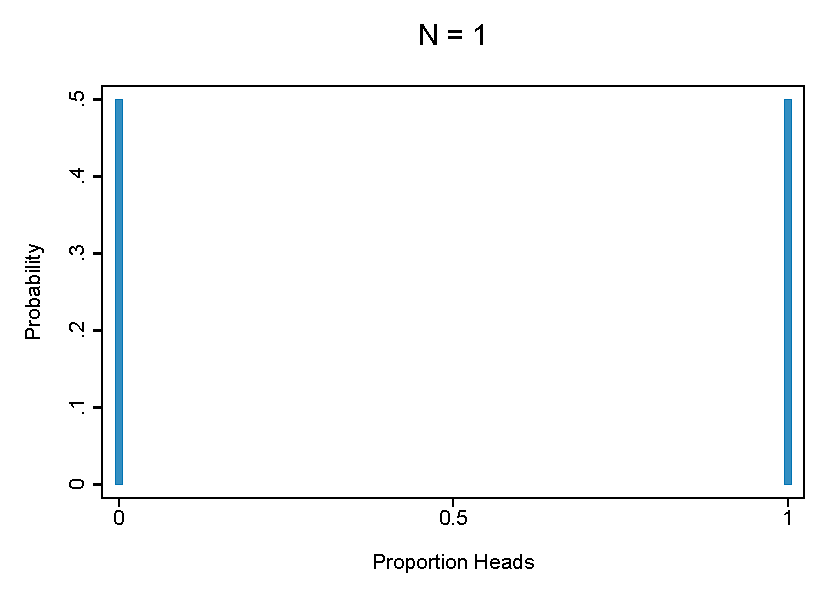
\includegraphics[width=0.64\textwidth]{fig/coinexample1.pdf}}
	\only<beamer>{\only<2>{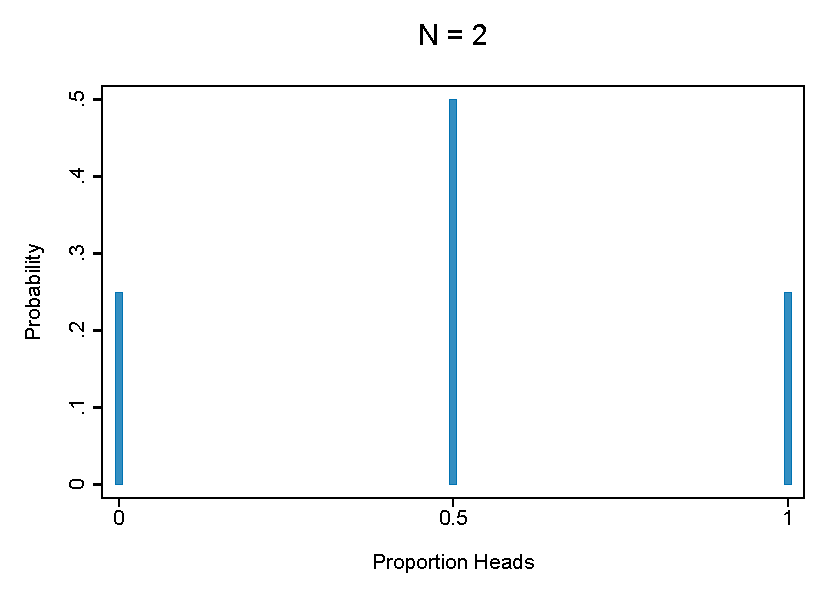
\includegraphics[width=0.64\textwidth]{fig/coinexample2.pdf}}}
\end{center}

%\medskip
The \textbf{Law of Large Numbers}: a sample average can be brought as close as we like to population mean just by increasing sample size

\end{frame}


\noindent
\HRule

\medskip
\noindent
Consider flipping a fair coin once:  the probability that it lands on heads is one half, but in any given flip (i.e.~data set with $N=1$) the coin will either land on heads 0 percent of the time or 100 percent of the time.

\end{frame}


%%%%%%%%%%%%%%%%%%%%%%%%%%%%%%%%%%%%%%%%%%%%%%%%%%%%%%%%%%%%%%%%%%%%%

\begin{frame}{Random Assignment \& the Law of Large Numbers}

\medskip

\begin{center}
	\begin{tabular}{cc}
		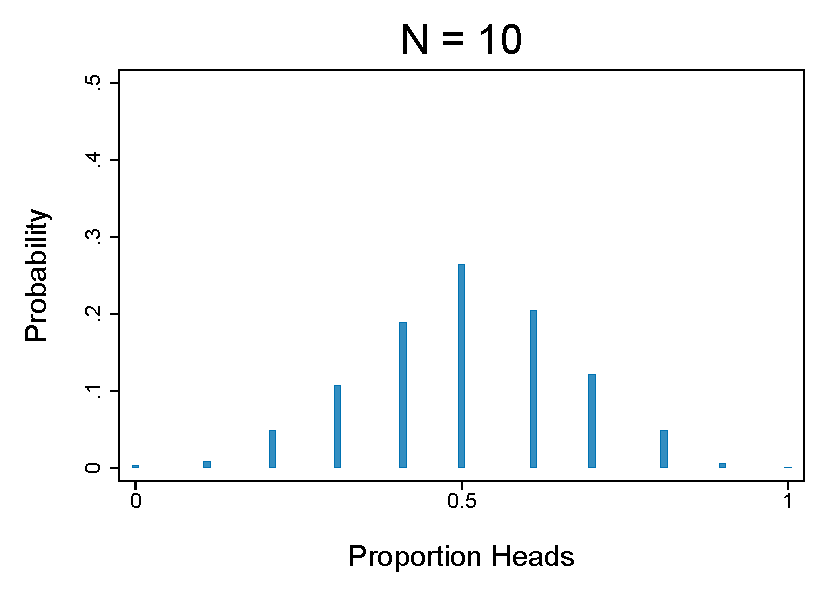
\includegraphics[width=0.4\textwidth]{fig/coinexample10.pdf}
		&
		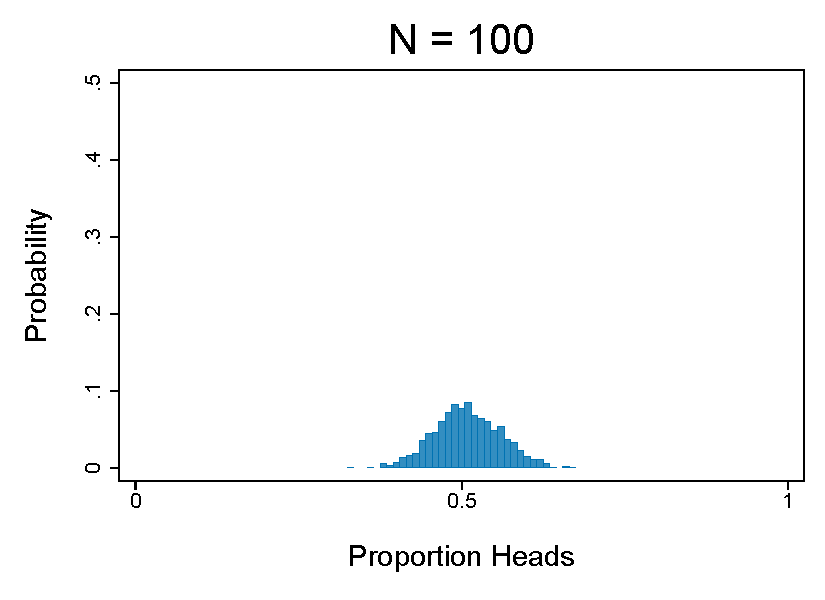
\includegraphics[width=0.4\textwidth]{fig/coinexample100.pdf} \\
		& \\
		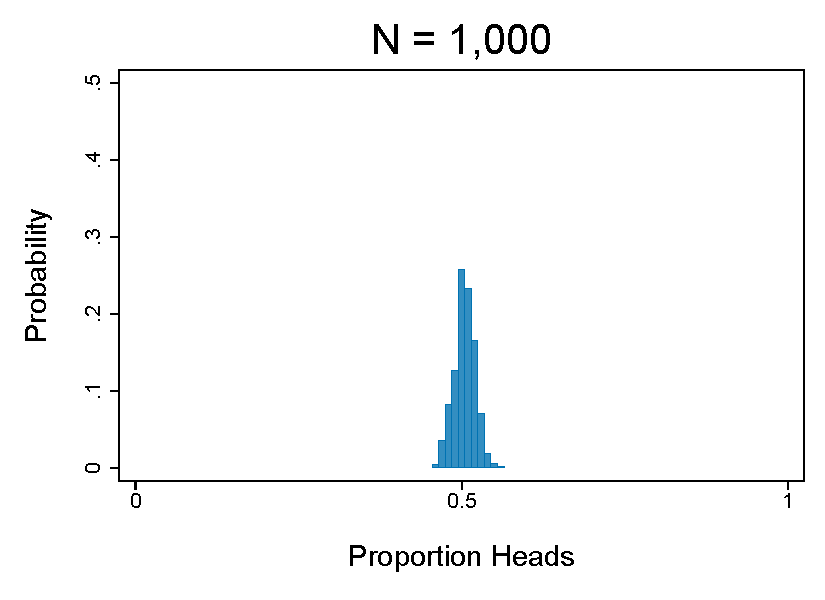
\includegraphics[width=0.4\textwidth]{fig/coinexample1000.pdf}
		&
		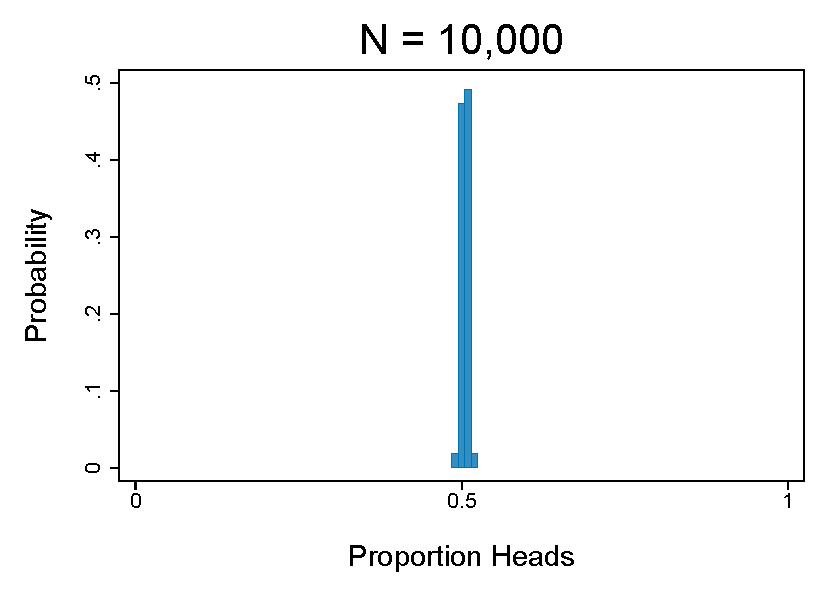
\includegraphics[width=0.4\textwidth]{fig/coinexample10000.pdf}	  \\
	\end{tabular}
\end{center}

%The \textbf{Law of Large Numbers}: a sample average can be brought as close as we like to population mean just by increasing sample size

\end{frame}



%%%%%%%%%%%%%%%%%%%%%%%%%%%%%%%%%%%%%%%%%%%%%%%%%%%%%%%%%%%%%%%%%%%%%

\begin{frame}{Random Assignment Eliminates Selection Bias}

\begin{center}
	\begin{tikzpicture}
	
	% blank canvas
	\only<handout>{\fill[fill=white,draw=white,ultra thin]
	(0,0) -- (11,0) -- (11,6.25) -- (0,6.25) -- cycle;}
	\only<beamer>{\fill[fill=white,draw=white,ultra thin]
	(0,0) -- (14,0) -- (14,6.25) -- (0,6.25) -- cycle;}
	%\only<beamer>{\draw[draw=oiblue!60,fill=oiblue!10,opacity=0.5] (11,1) rectangle (14,5);}
	%\draw[step=1.0,gray!20,thin] (0,0) grid (11,6);
	
	%\pgfmathsetmacro\xshift{0.5cm};
	%\pgfmathsetmacro\yshift{5.5cm};
	
	\pgfmathsetmacro\mycolor{"oiblue"};
	\filldraw[\mycolor] (9.97,3.84) circle[radius=0.1cm];
	\filldraw[\mycolor] (2.32,5.84) circle[radius=0.1cm];
	\filldraw[\mycolor] (9.51,3.99) circle[radius=0.1cm];
	\filldraw[\mycolor] (2.06,5.49) circle[radius=0.1cm];
	\filldraw[\mycolor] (6.4,2.17) circle[radius=0.1cm];
	\filldraw[\mycolor] (2.94,5.27) circle[radius=0.1cm];
	\filldraw[\mycolor] (9.77,3.41) circle[radius=0.1cm];
	\filldraw[\mycolor] (9.67,5.02) circle[radius=0.1cm];
	\filldraw[\mycolor] (7.2,5.07) circle[radius=0.1cm];
	\filldraw[\mycolor] (1.16,3.68) circle[radius=0.1cm];
	\filldraw[\mycolor] (2.06,2.45) circle[radius=0.1cm];
	\filldraw[\mycolor] (3.74,3.61) circle[radius=0.1cm];
	\filldraw[\mycolor] (3.14,4.82) circle[radius=0.1cm];
	\filldraw[\mycolor] (2.35,4.29) circle[radius=0.1cm];
	\filldraw[\mycolor] (8.24,2.4) circle[radius=0.1cm];
	\filldraw[\mycolor] (3.97,5.97) circle[radius=0.1cm];
	\filldraw[\mycolor] (4.81,3.48) circle[radius=0.1cm];
	\filldraw[\mycolor] (7.77,4.45) circle[radius=0.1cm];
	\filldraw[\mycolor] (8.96,5.57) circle[radius=0.1cm];
	\filldraw[\mycolor] (5.75,4.24) circle[radius=0.1cm];
	\filldraw[\mycolor] (7.49,3.88) circle[radius=0.1cm];
	
\pgfmathsetmacro\mycolor{"oiverm"};
\filldraw[\mycolor] (6.53,4.11) circle[radius=0.2cm];
\filldraw[\mycolor] (2.18,3.71) circle[radius=0.2cm];
\filldraw[\mycolor] (7.65,5.68) circle[radius=0.2cm];
\filldraw[\mycolor] (8.8,3.93) circle[radius=0.2cm];
\filldraw[\mycolor] (7.14,3.02) circle[radius=0.2cm];
\filldraw[\mycolor] (3.49,4) circle[radius=0.2cm];
\filldraw[\mycolor] (2.04,3.26) circle[radius=0.2cm];
\filldraw[\mycolor] (3.15,2.97) circle[radius=0.2cm];
\filldraw[\mycolor] (2.4,5.11) circle[radius=0.2cm];
\filldraw[\mycolor] (6.16,2.84) circle[radius=0.2cm];

\node[anchor=north,align=center,text width = 9.5cm] (text1) at (5.5,1.5) {When treatment is randomly assigned: \\
	 $E [ Y_{0,i} \vert D_i = 1] = E [ Y_{0,i} \vert D_i = 0] = E [ Y_{0,i} ]$};
 \draw[oigreen,thick] (text1.north west) -- (text1.north east) -- (text1.south east) -- (text1.south west) -- cycle;
	
	\end{tikzpicture}
\end{center}
\end{frame}



%%%%%%%%%%%%%%%%%%%%%%%%%%%%%%%%%%%%%%%%%%%%%%%%%%%%%%%%%%%%%%%%%%%%%

\begin{frame}<handout:0>{Random Assignment Eliminates Selection Bias}

\begin{center}
	\begin{tikzpicture}
	
	% blank canvas
	\only<handout>{\fill[fill=white,draw=white,ultra thin]
		(0,0) -- (11,0) -- (11,6.25) -- (0,6.25) -- cycle;}
	\only<beamer>{\fill[fill=white,draw=white,ultra thin]
		(0,0) -- (14,0) -- (14,6.25) -- (0,6.25) -- cycle;}
	%\only<beamer>{\draw[draw=oiblue!60,fill=oiblue!10,opacity=0.5] (11,1) rectangle (14,5);}
	%\draw[step=1.0,gray!20,thin] (0,0) grid (11,6);
	
	%\pgfmathsetmacro\xshift{0.5cm};
	%\pgfmathsetmacro\yshift{5.5cm};
	
\pgfmathsetmacro\mycolor{"gray"};
\draw[\mycolor] (2.32cm-0.25cm,5.84cm-0.25cm) rectangle (2.32cm+0.25cm,5.84cm+0.25cm);
\draw[\mycolor] (2.06cm-0.25cm,5.49cm-0.25cm) rectangle (2.06cm+0.25cm,5.49cm+0.25cm);
\draw[\mycolor] (6.4cm-0.25cm,2.17cm-0.25cm) rectangle (6.4cm+0.25cm,2.17cm+0.25cm);
\draw[\mycolor] (1.16cm-0.25cm,3.68cm-0.25cm) rectangle (1.16cm+0.25cm,3.68cm+0.25cm);
\draw[\mycolor] (3.14cm-0.25cm,4.82cm-0.25cm) rectangle (3.14cm+0.25cm,4.82cm+0.25cm);
\draw[\mycolor] (2.35cm-0.25cm,4.29cm-0.25cm) rectangle (2.35cm+0.25cm,4.29cm+0.25cm);
\draw[\mycolor] (8.24cm-0.25cm,2.4cm-0.25cm) rectangle (8.24cm+0.25cm,2.4cm+0.25cm);
\draw[\mycolor] (4.81cm-0.25cm,3.48cm-0.25cm) rectangle (4.81cm+0.25cm,3.48cm+0.25cm);
\draw[\mycolor] (8.96cm-0.25cm,5.57cm-0.25cm) rectangle (8.96cm+0.25cm,5.57cm+0.25cm);
\draw[\mycolor] (7.49cm-0.25cm,3.88cm-0.25cm) rectangle (7.49cm+0.25cm,3.88cm+0.25cm);
\draw[\mycolor] (6.53cm-0.25cm,4.11cm-0.25cm) rectangle (6.53cm+0.25cm,4.11cm+0.25cm);
\draw[\mycolor] (2.18cm-0.25cm,3.71cm-0.25cm) rectangle (2.18cm+0.25cm,3.71cm+0.25cm);
\draw[\mycolor] (7.77cm-0.25cm,4.45cm-0.25cm) rectangle (7.77cm+0.25cm,4.45cm+0.25cm);
\draw[\mycolor] (3.49cm-0.25cm,4cm-0.25cm) rectangle (3.49cm+0.25cm,4cm+0.25cm);	
\draw[\mycolor] (2.04cm-0.25cm,3.26cm-0.25cm) rectangle (2.04cm+0.25cm,3.26cm+0.25cm);
	
	\pgfmathsetmacro\mycolor{"oiblue"};
	\filldraw[\mycolor] (9.97,3.84) circle[radius=0.1cm];
	\filldraw[\mycolor] (2.32,5.84) circle[radius=0.1cm];
	\filldraw[\mycolor] (9.51,3.99) circle[radius=0.1cm];
	\filldraw[\mycolor] (2.06,5.49) circle[radius=0.1cm];
	\filldraw[\mycolor] (6.4,2.17) circle[radius=0.1cm];
	\filldraw[\mycolor] (2.94,5.27) circle[radius=0.1cm];
	\filldraw[\mycolor] (9.77,3.41) circle[radius=0.1cm];
	\filldraw[\mycolor] (9.67,5.02) circle[radius=0.1cm];
	\filldraw[\mycolor] (7.2,5.07) circle[radius=0.1cm];
	\filldraw[\mycolor] (1.16,3.68) circle[radius=0.1cm];
	\filldraw[\mycolor] (2.06,2.45) circle[radius=0.1cm];
	\filldraw[\mycolor] (3.74,3.61) circle[radius=0.1cm];
	\filldraw[\mycolor] (3.14,4.82) circle[radius=0.1cm];
	\filldraw[\mycolor] (2.35,4.29) circle[radius=0.1cm];
	\filldraw[\mycolor] (8.24,2.4) circle[radius=0.1cm];
	\filldraw[\mycolor] (3.97,5.97) circle[radius=0.1cm];
	\filldraw[\mycolor] (4.81,3.48) circle[radius=0.1cm];
	\filldraw[\mycolor] (7.77,4.45) circle[radius=0.1cm];
	\filldraw[\mycolor] (8.96,5.57) circle[radius=0.1cm];
	\filldraw[\mycolor] (5.75,4.24) circle[radius=0.1cm];
	\filldraw[\mycolor] (7.49,3.88) circle[radius=0.1cm];
	
	\pgfmathsetmacro\mycolor{"oiverm"};
	\filldraw[\mycolor] (6.53,4.11) circle[radius=0.2cm];
	\filldraw[\mycolor] (2.18,3.71) circle[radius=0.2cm];
	\filldraw[\mycolor] (7.65,5.68) circle[radius=0.2cm];
	\filldraw[\mycolor] (8.8,3.93) circle[radius=0.2cm];
	\filldraw[\mycolor] (7.14,3.02) circle[radius=0.2cm];
	\filldraw[\mycolor] (3.49,4) circle[radius=0.2cm];
	\filldraw[\mycolor] (2.04,3.26) circle[radius=0.2cm];
	\filldraw[\mycolor] (3.15,2.97) circle[radius=0.2cm];
	\filldraw[\mycolor] (2.4,5.11) circle[radius=0.2cm];
	\filldraw[\mycolor] (6.16,2.84) circle[radius=0.2cm];
	
	\node[anchor=north,align=center,text width = 9.5cm] (text1) at (5.5,1.5) {When treatment is randomly assigned: \\
		$E [ Y_{0,i} \vert D_i = 1] = E [ Y_{0,i} \vert D_i = 0] = E [ Y_{0,i} ]$};
	\draw[oigreen,thick] (text1.north west) -- (text1.north east) -- (text1.south east) -- (text1.south west) -- cycle;
	
	\end{tikzpicture}
\end{center}
\end{frame}




%%%%%%%%%%%%%%%%%%%%%%%%%%%%%%%%%%%%%%%%%%%%%%%%%%%%%%%%%%%%%%%%%%%%%

\begin{frame}{Random Assignment Eliminates Selection Bias}

\medskip
Difference in means (treatment - control) provides an unbiased estimate of 
the (casual) \textbf{average treatment effect} (or ATE):
\medskip
\begin{small}
	\begingroup
	\addtolength{\jot}{1em}
	\begin{align*}
	&= E [ Y_i \vert D_i = 1 ] - E [ Y_i \vert D_i = 0 ]\\
	& = E [ Y_{\color{red}1 \color{black},i} \vert D_i = \color{red}1\color{black} ]
	- E [ Y_{\color{red}0\color{black},i} \vert D_i = \color{red}0\color{black} ] \\
	&= E [ Y_{\color{red}1 \color{black},i} \vert D_i = \color{red}1\color{black} ]
	- E [ Y_{\color{red}0\color{black},i} \vert D_i = \color{red}1\color{black} ]
	+ E [ Y_{\color{red}0\color{black},i} \vert D_i = \color{red}1\color{black} ]
	- E [ Y_{\color{red}0\color{black},i} \vert D_i = \color{red}0\color{black} ] \\
	&= \underbrace{E [ Y_{\color{red}1 \color{black},i} \vert D_i = \color{red}1\color{black} ]
		- E [ Y_{\color{red}0\color{black},i} \vert D_i = \color{red}1\color{black} ]}_{\textsf{average treatment effect on participants}}
	+ \underbrace{E [ Y_{\color{red}0\color{black},i} ] - E [ Y_{\color{red}0\color{black},i}  ]}_{=0} \\
	&= \underbrace{E [ Y_{\color{red}1 \color{black},i} ] - E [ Y_{\color{red}0 \color{black},i} ]}_{\textsf{ATE}}
	\end{align*}
	\endgroup
\end{small}


\end{frame}



%%%%%%%%%%%%%%%%%%%%%%%%%%%%%%%%%%%%%%%%%%%%%%%%%%%%%%%%%%%%%%%%%%%%%

\begin{frame}{Internal Validity}

\medskip
Excellent news:  random assignment eliminates selection bias$^{\ast}$\\
\begin{footnotesize}$^{\ast}$Some restrictions apply \end{footnotesize}

\pause
\medskip
\medskip
The \textbf{Stable Unit Treatment Value Assumption (SUTVA)}:

\medskip
\begin{itemize}
	
	\item ``The potential outcomes for any unit do not vary with the treatments assigned to other units'' (Imbens and Rubin 2015)
	
	%\item ``There are no different forms or versions of each treatment level which lead to different potential outcomes.''
	
	%\item[$\ $] \emph{Source:  Imbens and Rubin (2015)}
	
\end{itemize}

\pause
\medskip
\medskip
\textbf{When is SUTVA likely to be violated? }

\medskip
\begin{itemize}
	
	\item When there are spillovers (so $i$'s treatment impacts $j$)
	
	\item Example:  vaccination(!) and other health treatments
	
\medskip
\begin{itemize}
	
	\item This is why we have ``cluster-randomized'' trials
	
\end{itemize}
	
\end{itemize}


\end{frame}


%%%%%%%%%%%%%%%%%%%%%%%%%%%%%%%%%%%%%%%%%%%%%%%%%%%%%%%%%%%%%%%%%%%%%

\begin{frame}{The Punchline}

\medskip
When treatment is randomly assigned (at an appropriate level), difference in outcomes between treatment and control groups provides an unbiased estimate of the causal impact of treatment

\medskip
\medskip
Randomly assigning treatment status eliminates selection bias \\
(at least in expectation) because treatment, control groups are random samples of same underlying population of eligible units

\end{frame}


%%%%%%%%%%%%%%%%%%%%%%%%%%%%%%%%%%%%%%%%%%%%%%%%%%%%%%%%%%%%%%%%%%%%%%%%%%%%

%\begin{frame}<handout:0>[bg,plain]
\begin{frame}[plain]
%\only<beamer>{\begin{adjustwidth}{0cm}{-4cm}}
\begin{center}
	
	\Large{\textcolor{williams}{Randomization:  A Short History}}
	
\end{center}
%\only<beamer>{\end{adjustwidth}}
\end{frame}


%%%%%%%%%%%%%%%%%%%%%%%%%%%%%%%%%%%%%%%%%%%%%%%%%%%%%%%%%%%%%%%%%%%%%

\begin{frame}{Randomized Experiments in Theory}

\medskip
Petrarch (1364):

\begin{center}
	\begin{small}
		\emph{``If a hundred thousand men of the same age, same temperament and habits, 
			together with the same surroundings, were attacked at the same time 
			by the same disease, that if one half followed the prescriptions of the doctors 
			of the variety of those practicing at the present day, and that the other half took no medicine but relied on nature's instincts, I have no doubt as to which half would escape.''}
		
	\end{small}
\end{center}

\pause
\medskip
van Helmont (who died in 1644):

\begin{center}
	\begin{small}
		\emph{``Let us take out of the Hospitals, pit of the Camps, or from elsewhere, 
			200 or 500 poor People, that have Fevers, Pleurisies, etc. Let us divide them 
			in halfes, let us cast lots, that one half of them may fall to my share, 
			and the other to yours; I will cure them without bloodletting... \\
			we shall see 
			how many Funerals both of us shall have.''}
	\end{small}
\end{center}

\medskip
\scriptsize{\emph{Source:  Jamison (2019)}}

\end{frame}


%%%%%%%%%%%%%%%%%%%%%%%%%%%%%%%%%%%%%%%%%%%%%%%%%%%%%%%%%%%%%%%%%%%%%

\begin{frame}{Randomization:  A Timeline (Part I)}

\medskip
\begin{small}
	\begin{itemize}
		
		\item[1885] Pierce and Jastrow use randomization in a psychology experiment (varying order in which different stimuli are presented to subjects)
		
		\item[1898] Johannes Fibiger conducts a trial of an anti-diphtheria serum in which every other subject is assigned to treatment (or control)
		
		\item[1923] Neyman suggests the idea of potential outcomes
		
		\item[1925] \structure{\textbf{Fisher suggests the explicit randomization of treatments}} \\
		\structure{\textbf{(in the context of agriculture experiments)}}
		
		\item[1926] Amberson et al.~study of sanocrysin treatments for TB:  coin flipped to determine which group received treatment, which were controls
		
		\item[1948] Randomized trial of streptomycin treatment for TB conducted by the Medical Research Council of Great Britain
		
		\medskip
		\begin{itemize}
			
			\item[$\Rightarrow$] Randomized evaluations become the norm in medicine
			
		\end{itemize}
		
		%\item[1926] Amberson \emph{et al} study of sanocrysin treatments for TB:  24 patients divided into two comparable groups; coin flipped to determine which group of 12 receives treatment and which group serves as controls
		
		%\item[1942] Launch of Cambridge-Somerville Youth Study of at-risk boys
		%
		%\item[1948] Randomized trial of streptomycin treatment for TB conducted by the Medical Research Council of Great Britain
		%
		%\item[1962] Perry preschool experiment in Ypsilanti, MI
		%
		%\item[1974] Rubin introduces the concept of potential outcomes (as we know it)
		
	\end{itemize}
\end{small}

\end{frame}


%%%%%%%%%%%%%%%%%%%%%%%%%%%%%%%%%%%%%%%%%%%%%%%%%%%%%%%%%%%%%%%%%%%%%

\begin{frame}{The Lady Tasting Tea}

\begin{center}
\begin{tikzpicture}
	
	% blank canvas
	\only<handout>{\fill[fill=white,draw=white,ultra thin]
	(0,0) -- (11,0) -- (11,6) -- (0,6) -- cycle;}
	\only<beamer>{\fill[fill=white,draw=white,ultra thin]
	(0,0) -- (14,0) -- (14,6) -- (0,6) -- cycle;}
	\only<beamer>{\draw[draw=oiblue!60,fill=oiblue!10,opacity=0.5] (11,1) rectangle (14,5);}
	%\draw[step=1.0,gray!20,thin] (0,0) grid (11,6);
	
	\pgfmathsetmacro\xshift{0cm};
	\pgfmathsetmacro\yshift{2.125cm};
%	\pgfmathsetmacro\mycolor{"gray"};
	
\node[anchor=north west,align=left,text width = 9.5cm,xshift=\xshift,yshift=\yshift] (text1) at (0,0) {Chapter II of Fisher's \emph{The Design of Experiments} begins:};

\node[anchor=north,align=center,text width = 9.5cm,xshift=\xshift,yshift=\yshift] (text2) at (5,-0.625) {\emph{``A lady declares that by tasting a cup of tea made with milk \\
		she can discriminate whether the milk or the tea infusion \\
		was first added to the cup.''}};
	
	
\node [anchor=north] at (5,5.75) {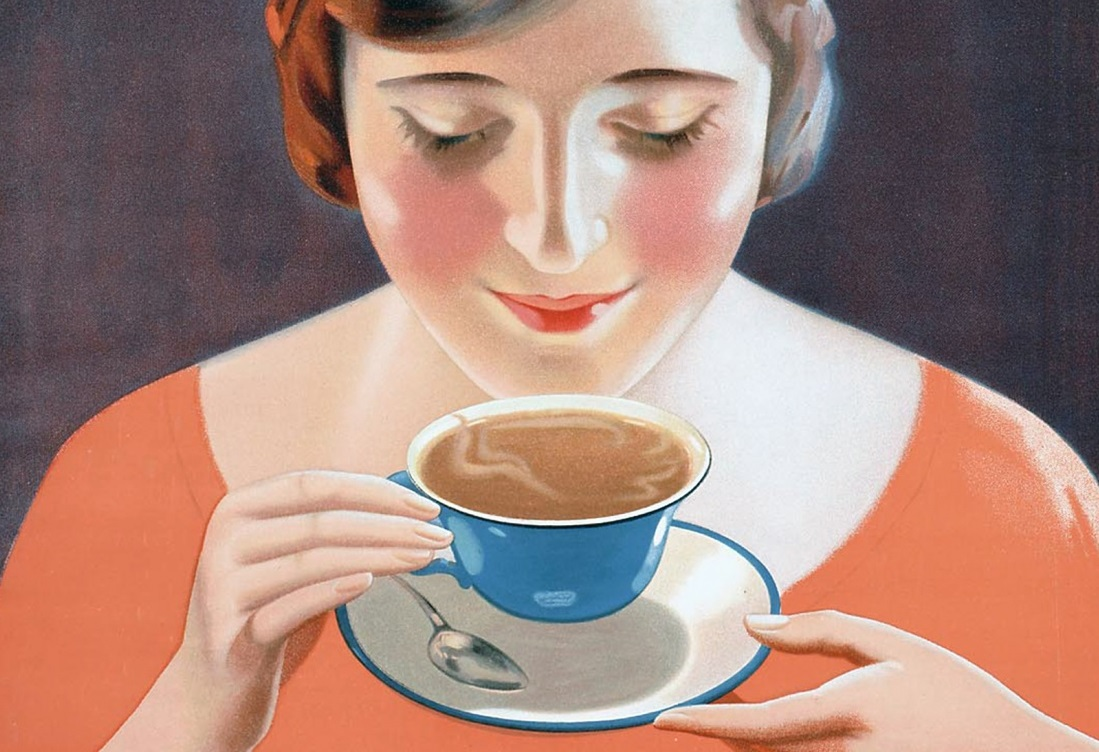
\includegraphics[keepaspectratio,height=3.0cm]{img/public-domain-tea-advert-crop.jpg}};
	
\end{tikzpicture}
\end{center}

\end{frame}


%%%%%%%%%%%%%%%%%%%%%%%%%%%%%%%%%%%%%%%%%%%%%%%%%%%%%%%%%%%%%%%%%%%%%

\begin{frame}<handout:0>{The Lady Tasting Tea}

\begin{center}
	\begin{tikzpicture}
	
	% blank canvas
	\only<handout>{\fill[fill=white,draw=white,ultra thin]
		(0,0) -- (11,0) -- (11,6) -- (0,6) -- cycle;}
	\only<beamer>{\fill[fill=white,draw=white,ultra thin]
		(0,0) -- (14,0) -- (14,6) -- (0,6) -- cycle;}
	\only<beamer>{\draw[draw=oiblue!60,fill=oiblue!10,opacity=0.5] (11,1) rectangle (14,5);}
	%\draw[step=1.0,gray!20,thin] (0,0) grid (11,6);
	
	\pgfmathsetmacro\xshift{0cm};
	\pgfmathsetmacro\yshift{2.125cm};
	%	\pgfmathsetmacro\mycolor{"gray"};
	
	\node[anchor=north west,align=left,text width = 9.5cm,xshift=\xshift,yshift=\yshift] (text1) at (0,0) {Chapter II of Fisher's \emph{The Design of Experiments} begins:};
	
	\node[anchor=north,align=center,text width = 9.5cm,xshift=\xshift,yshift=\yshift] (text2) at (5,-0.625) {\emph{``A lady declares that by tasting a cup of tea made with milk \\
			she can discriminate whether the milk or the tea infusion \\
			was first added to the cup.''}};
	
	
	\node [anchor=north east] at (4.9,5.875) {\fbox{
\includegraphics[keepaspectratio,height=3.0cm]{img/fisher-tweet.png}}};
	%\node [anchor=north west] at (5.1,5.875) {\fbox{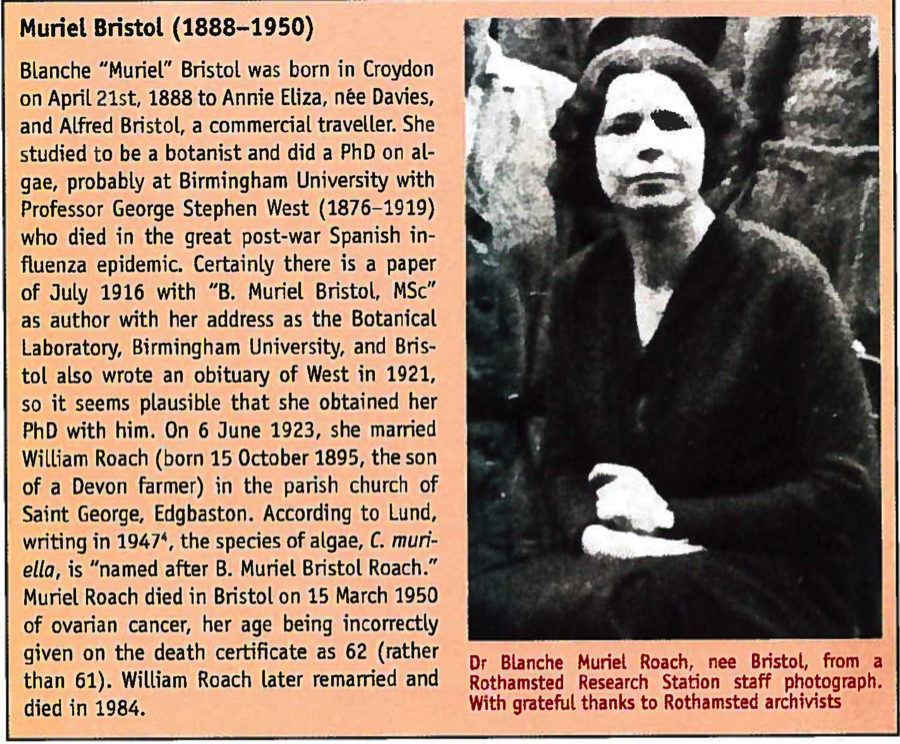
\includegraphics[keepaspectratio,height=3.0cm]{img/bristol.png}}};
	
	\end{tikzpicture}
\end{center}

\end{frame}



%%%%%%%%%%%%%%%%%%%%%%%%%%%%%%%%%%%%%%%%%%%%%%%%%%%%%%%%%%%%%%%%%%%%%

\begin{frame}<handout:0>{The Lady Tasting Tea}

\begin{center}
	\begin{tikzpicture}
	
	% blank canvas
	\only<handout>{\fill[fill=white,draw=white,ultra thin]
		(0,0) -- (11,0) -- (11,6) -- (0,6) -- cycle;}
	\only<beamer>{\fill[fill=white,draw=white,ultra thin]
		(0,0) -- (14,0) -- (14,6) -- (0,6) -- cycle;}
	\only<beamer>{\draw[draw=oiblue!60,fill=oiblue!10,opacity=0.5] (11,1) rectangle (14,5);}
	%\draw[step=1.0,gray!20,thin] (0,0) grid (11,6);
	
	\pgfmathsetmacro\xshift{0cm};
	\pgfmathsetmacro\yshift{2.125cm};
	%	\pgfmathsetmacro\mycolor{"gray"};
	
	\node[anchor=north west,align=left,text width = 9.5cm,xshift=\xshift,yshift=\yshift] (text1) at (0,0) {Chapter II of Fisher's \emph{The Design of Experiments} begins:};
	
	\node[anchor=north,align=center,text width = 9.5cm,xshift=\xshift,yshift=\yshift] (text2) at (5,-0.625) {\emph{``A lady declares that by tasting a cup of tea made with milk \\
			she can discriminate whether the milk or the tea infusion \\
			was first added to the cup.''}};
	
	
	\node [anchor=north east] at (4.9,5.875) {\fbox{
\includegraphics[keepaspectratio,height=3.0cm]{img/fisher-tweet.png}}};
	\node [anchor=north west] at (5.1,5.875) {\fbox{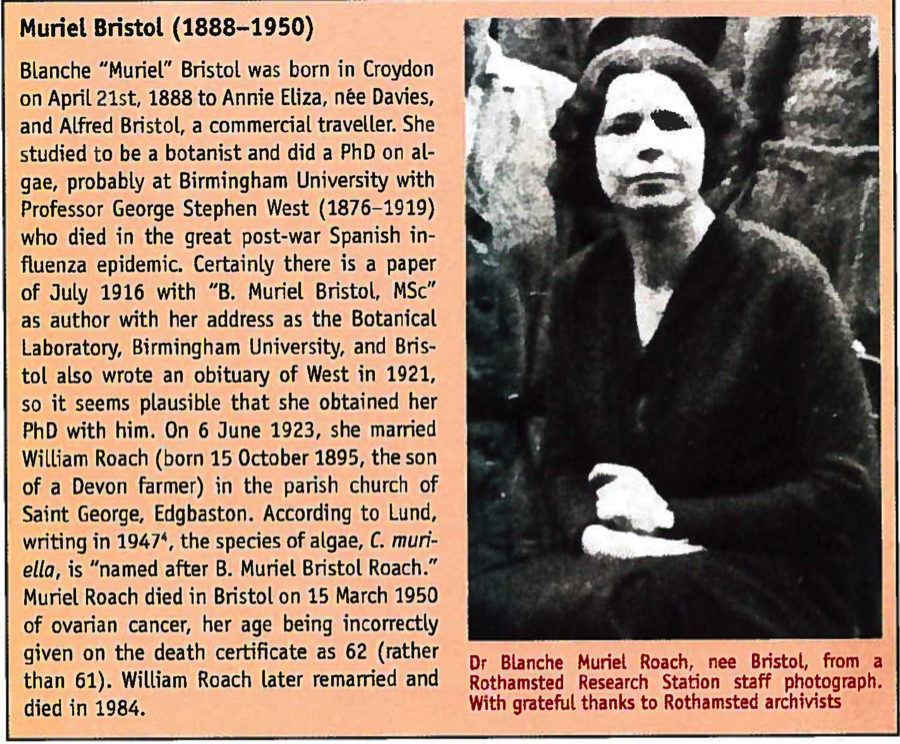
\includegraphics[keepaspectratio,height=3.0cm]{img/bristol.png}}};
	
	\end{tikzpicture}
\end{center}

\end{frame}



%%%%%%%%%%%%%%%%%%%%%%%%%%%%%%%%%%%%%%%%%%%%%%%%%%%%%%%%%%%%%%%%%%%%%

\begin{frame}{The Lady Tasting Tea}

%\medskip
%Chapter II of Fisher's \emph{The Design of Experiments} begins:
%
%\medskip
%\begin{center}
%	\emph{``A lady declares that by tasting a cup of tea made with milk \\
%		she can discriminate whether the milk or the tea infusion \\
%		was first added to the cup.''}
%\end{center}

%\pause
%\medskip
%\textbf{Critical lesson to take away from this anecdote:}  
%caffeine breaks with your colleagues are critical to the advancement of science

\medskip
\textbf{Null hypothesis} (aka $H_0$)

\medskip
\begin{itemize}
	
	%\item The lady in question was biologist Muriel Bristol, who worked with Fisher at the Rothamsted Experimental Station 
	
	\item Fisher believes that Dr.~Bristol cannot taste the difference
	
\end{itemize}

\pause
\medskip
\medskip
A test of the hypothesis:

\medskip
\begin{itemize}
	
	%\item The lady in question was biologist Muriel Bristol, who worked with Fisher at the Rothamsted Experimental Station 
	
	\item
	\emph{``Our experiment consists in mixing eight cups of tea, \\
		four in one way and four in the other, and presenting them \\
		to the subject for judgment in random order.''}
	
\end{itemize}

\end{frame}


%%%%%%%%%%%%%%%%%%%%%%%%%%%%%%%%%%%%%%%%%%%%%%%%%%%%%%%%%%%%%%%%%%%%%

\begin{frame}{The Lady Tasting Tea:  Experimental Design}

\medskip
\textbf{Rule \#1:  do not confound your own treatment}

\medskip
\begin{itemize}
	
	\item Critical assumption: if Dr.~Bristol is unable to detect whether the milk was poured in first, she will choose 4 cups at random
	
	\item Fisher points out that the experimenter could screw this up:
	
	\medskip
	\begin{center}
		\emph{``If all those cups made with the milk first had sugar added, \\
			while those made with the tea first had none, \\
			a very obvious difference in flavour would have been introduced \\
			which might well ensure that all those made with sugar \\
			should be classed alike.''}
	\end{center}
	
	\pause
	%\medskip
	\item Gerber and Green refer to this as \textbf{excludability}
	
\end{itemize}

\end{frame}


%%%%%%%%%%%%%%%%%%%%%%%%%%%%%%%%%%%%%%%%%%%%%%%%%%%%%%%%%%%%%%%%%%%%%

\begin{frame}{The Lady Tasting Tea:  Experimental Design}

\medskip
\textbf{Rule \#1B:  do not \underline{accidentally} confound your own treatment}

\medskip
\begin{itemize}
	
	\item Fisher, in (perhaps) the earliest known scientific subtweet:
	
	\medskip
	\begin{center}
		\emph{``It is not sufficient remedy to insist that `all the cups \\
			must be exactly alike' in every respect except that to be tested.  \\
			For this is a totally impossible requirement.''}
	\end{center}
	
	\pause
	\medskip
	\item To minimize likelihood of accidentally confounding your treatment, it's best is to constrain yourself by randomizing
	
	\medskip
	\begin{itemize}
		
		\item Minimizes the likelihood of unfortunate coincidences
		
		\item Highly controversial position at the time, and is still debated in some circles; alternative is to force balance on observables \\ (and then just hope that unobservables don't matter too much)
		
	\end{itemize}
	
\end{itemize}

\end{frame}


%%%%%%%%%%%%%%%%%%%%%%%%%%%%%%%%%%%%%%%%%%%%%%%%%%%%%%%%%%%%%%%%%%%%%

\begin{frame}{The Lady Tasting Tea:  a Hypothesis Test}

\medskip
How should we interpret data from this experiment?

\pause
\medskip
\medskip
\textbf{Suppose Dr.~Bristol correctly identified all 4 ``treated'' cups}

\medskip
\begin{itemize}
	
	\item How likely is it that this could have occurred by chance?
	
	\medskip
	\begin{itemize}
		
		\item There are ${8 \choose 4} = 70$ possible ways to choose 4 of 8 cups
		
		\item Only one is correct; a subject with no ability to discriminate between treated, untreated cups has a 1/70 chance of success
		
		\item The p-value associated with this outcome is 1/70 $\approx 0.014$, less than the cutoff for the ``standard level of significance'' of 0.05
		
	\end{itemize}
	
\end{itemize}

\end{frame}

%%%%%%%%%%%%%%%%%%%%%%%%%%%%%%%%%%%%%%%%%%%%%%%%%%%%%%%%%%%%%%%%%%%%%

\begin{frame}{The Lady Tasting Tea:  a Hypothesis Test}

%\medskip
%How should we interpret data from this experiment?
%
%\pause
%\medskip
\medskip
\textbf{Suppose Dr.~Bristol correctly identified 3 ``treated'' cups}

\medskip
\begin{itemize}
	
	\item How likely is it that this could have occurred by chance?
	
	\medskip
	\begin{itemize}
		
		\item There are ${4 \choose 3} \times {4 \choose 1} = 16$ possible ways to choose 3 of 8 cups
		
		\medskip
		\begin{itemize}
			
			\item There are 17 ways to choose \textbf{at least} 3 correct cups
			
		\end{itemize}
		
		\item The p-value associated with this outcome is 17/70 $\approx 0.243$
		
		\item We should not reject the null hypothesis
		
	\end{itemize}
	
\end{itemize}

\pause
\medskip
\medskip
\textbf{Only reject $H_0$ if Dr.~Bristol identifies all 4 treated cups}

\medskip
\begin{itemize}
	
	\item In the actual experiment, the null hypothesis was rejected
	
\end{itemize}

\end{frame}


%%%%%%%%%%%%%%%%%%%%%%%%%%%%%%%%%%%%%%%%%%%%%%%%%%%%%%%%%%%%%%%%%%%%%%
%
%\begin{frame}{Fisher's Exact Test}
%
%\medskip
%\begin{small}
%	\begin{center}
%		\begin{tabular}{r|c|c|}
%			\multicolumn{1}{c}{$\ $}           & \multicolumn{2}{c}{\textbf{Identified by Dr.~Bristol?}} \\ [0.6ex]
%			\multicolumn{1}{c}{$\ $}           & \multicolumn{1}{c}{\textbf{Yes}}   & \multicolumn{1}{c}{\textbf{No}}     \\ \cline{2-3}
%			&  & \\
%			\textbf{Milk poured first}        &  $a$             &  $b$             \\
%			& & \\  \cline{2-3}
%			& & \\
%			\textbf{Tea poured first}    &  $c$             &  $d$             \\
%			& & \\  \cline{2-3}
%			\multicolumn{1}{c}{$\ $}           & \multicolumn{1}{p{0.8in}}{$\ $}    & \multicolumn{1}{p{0.8in}}{$\ $}     \\
%		\end{tabular}
%	\end{center}
%\end{small}
%
%\medskip
%Is Dr.~Bristol more likely to select cups where the milk was poured first?
%\begin{small}
%	\begin{equation*}
%	\textsf{probability} = \frac{\displaystyle{{a+b \choose a} {c+d \choose c}}}{\displaystyle{{a+b+c+d \choose a+c}}} = \frac{\displaystyle{(a+b)! (c+d)! (a+c)! (b+d)!}}{\displaystyle{a! b! c! d! (a+b+c+d)! }}
%	\end{equation*}
%\end{small}
%
%\medskip
%\textbf{The p-value is the sum of the probabilities of outcomes that are at least as extreme (i.e. contrary to $H_0$) as the observed outcome}
%
%\end{frame}


%%%%%%%%%%%%%%%%%%%%%%%%%%%%%%%%%%%%%%%%%%%%%%%%%%%%%%%%%%%%%%%%%%%%%

\begin{frame}{The Lady Tasting Tea:  Size and Power}

\medskip
The size of a test is the likelihood of rejecting a true null

\medskip
\begin{itemize}
	
	\item Fisher asserts that tests of size $0.05$ are typical
	
\end{itemize}

\pause
\medskip
\textbf{Alternative experiment:}  what if we had treated 3 out of 6 cups?

\medskip
\begin{itemize}
	
	\item There are ${6 \choose 3} = 20$ possible ways to choose 3 of 6 cups
	
	\item Best possible p-value is therefore $0.05$
	
\end{itemize}

\pause
\medskip
\textbf{Alternative experiment:}  what if we had treated 3 out of 8 cups?

\medskip
\begin{itemize}
	
	\item There are ${8 \choose 3} = 56$ possible ways to choose 3 of 8 cups
	
	\item Best possible p-value is therefore $0.017$
	
\end{itemize}

\pause
\medskip
$\Rightarrow$ \textbf{Optimal to have equal numbers of treated, untreated cups}

\end{frame}


%%%%%%%%%%%%%%%%%%%%%%%%%%%%%%%%%%%%%%%%%%%%%%%%%%%%%%%%%%%%%%%%%%%%%

\begin{frame}{The Lady Tasting Tea:  Size and Power}

\medskip
\textbf{An alternate experiment:} an unknown number of treated cups

\medskip
\begin{itemize}
	
	\item Under the null, the probability of getting 8 right is 1 in $2^8$
	
	\item Probability of getting 7 right is $8/256 = 0.03125$
	
\end{itemize}

\pause
\medskip
Design would achieve higher power with the same number of trials

\medskip
\begin{itemize}
	
	\item Possible to reject the hypothesis that Dr.~Bristol cannot tell the difference even when her ability to discriminate is imperfect
	
\end{itemize}


\end{frame}


%%%%%%%%%%%%%%%%%%%%%%%%%%%%%%%%%%%%%%%%%%%%%%%%%%%%%%%%%%%%%%%%%%%%%

\begin{frame}{Ronald Fisher's Contributions to Statistics}

\medskip
\textbf{Key lesson to take away from ``lady tasting tea'' anecdote:}  \\
caffeine breaks with colleagues critical to advancement of science

\pause
\medskip
\medskip
Other contributions:

\medskip
\begin{enumerate}
	
	\item Introduced the modern randomized trial
	
	\item Introduced the idea of permutation tests
	
\end{enumerate}

\medskip
Fisher's permutation-based approach to inference is not the norm in economics; our default is regression analysis and classical statistics

\end{frame}



%%%%%%%%%%%%%%%%%%%%%%%%%%%%%%%%%%%%%%%%%%%%%%%%%%%%%%%%%%%%%%%%%%%%%

\begin{frame}{Randomization:  A Timeline (Part II)}

\medskip
\begin{small}
	\begin{itemize}
		
		%		\item[1885] Pierce and Jastrow use randomization in a psychology experiment (varying order in which different stimuli are presented to subjects)
		%		
		%		\item[1898] Johannes Fibiger conducts a trial of an anti-diphtheria serum in which every other subject is assigned to treatment (or control)
		%		
		%		\item[1923] Neyman suggests the idea of potential outcomes
		%		
		%		\item[1925] Fisher suggests the explicit randomization of treatments\\
		%		(in the context of agriculture experiments)
		%		
		%		\item[1926] Amberson \emph{et al} study of sanocrysin treatments for TB:  coin flipped to determine which group  receives treatment, which group serves as controls
		
		%\item[1926] Amberson \emph{et al} study of sanocrysin treatments for TB:  24 patients divided into two comparable groups; coin flipped to determine which group of 12 receives treatment and which group serves as controls
		
		\item[1942] Launch of Cambridge-Somerville Youth Study of at-risk boys
		
		
		\item[1962] Perry Preschool (MI) and Early Training Project (TN) experiments randomize assignment of at-risk children to high-quality preschools 
		
		\item[1967] NJ Income Maintenance Experiment (proposed by Heather Ross), \\
		4 other negative income tax experiments between 1971 and 1982
		
		\item[1972] Abecedarian Project (NC) randomized intervention for at-risk infants 
		
		\item[1974] Rubin introduces the concept of potential outcomes (as we know it)
		
		\item[1994] National Job Corps Study (by Mathematica/US Dept.~of Labor)
		
		\item[1995] PROGRESA evaluation launched by Mexican government
		
		\item[1998] Dutch NGO ICS Africa begins randomized trial of ``deworming'' in Kenyan primary schools... in partnership with Michael Kremer
		
	\end{itemize}
\end{small}

\end{frame}


%%%%%%%%%%%%%%%%%%%%%%%%%%%%%%%%%%%%%%%%%%%%%%%%%%%%%%%%%%%%%%%%%%%%%

\begin{frame}{RCTs in Development Economics:  Mexico's Progresa}

\begin{center}
	\begin{tikzpicture}
	
	% blank canvas
	\only<handout>{\fill[fill=white,draw=white,ultra thin]
		(0,0) -- (11,0) -- (11,6) -- (0,6) -- cycle;}
	\only<beamer>{\fill[fill=white,draw=white,ultra thin]
		(0,0) -- (14,0) -- (14,6) -- (0,6) -- cycle;}
	\only<beamer>{\draw[draw=oiblue!60,fill=oiblue!10,opacity=0.5] (11,1) rectangle (14,5);}
	%\draw[step=1.0,gray!20,thin] (0,0) grid (11,6);
	
	\node [anchor=north] (photo) at (5,5.875) {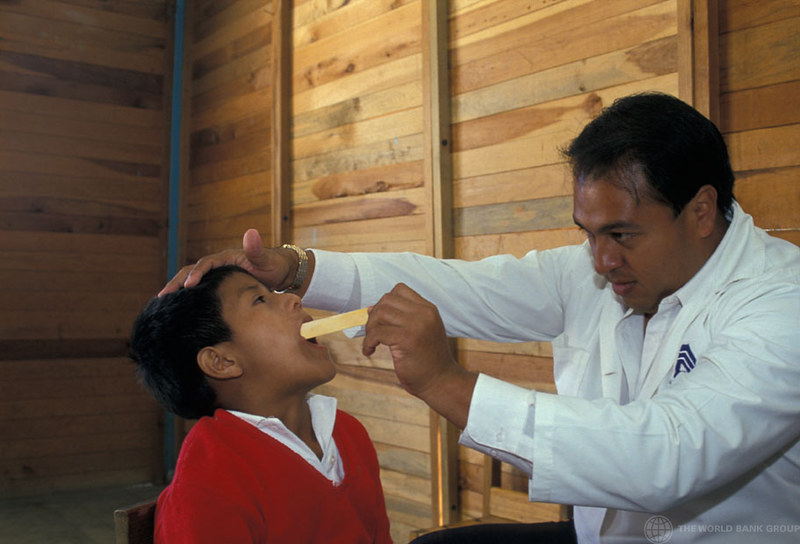
\includegraphics[keepaspectratio,height=3.0cm]{photos/Mexico-child-with-doctor-Curt-Carnemark-2008-MED.jpg}};
	\node [gray,anchor=north] at (photo.south) {\tiny{photo:  Curt Carnemark / World Bank}};
	
	\pgfmathsetmacro\xshift{0cm};
	\pgfmathsetmacro\yshift{2.5cm};
	%	\pgfmathsetmacro\mycolor{"gray"};
	
	%\node[anchor=north west,align=left,text width = 9.5cm,xshift=\xshift,yshift=\yshift] (text1) at (0,0) {\textbf{The Progresa Evaluation in Mexico}};
	
	\node[anchor=north west,align=left,text width = 9.5cm,xshift=\xshift,yshift=\yshift] (text2) at (0.5,-0.625) {\textcolor{structure}{$\bullet$} Mexico piloted conditional cash transfers (CCTs) in mid-1990s};	
	
	\node[anchor=north west,align=left,text width = 9.5cm,xshift=\xshift,yshift=\yshift] (text3) at (0.5,-1.25) {\textcolor{structure}{$\bullet$} Economists in gov't pushed for randomized roll out of pilot};	
	
	\node[anchor=north west,align=left,text width = 9.5cm,xshift=\xshift,yshift=\yshift] (text4) at (0.5,-1.875) {\textcolor{structure}{$\bullet$} IFPRI reserachers published initial findings in late 1990s };
	
	\end{tikzpicture}
\end{center}

\end{frame}


%%%%%%%%%%%%%%%%%%%%%%%%%%%%%%%%%%%%%%%%%%%%%%%%%%%%%%%%%%%%%%%%%%%%%

\begin{frame}{RCTs in Development Economics:  Busia, Kenya}

\begin{center}
	\begin{tikzpicture}
	
	% blank canvas
	\only<handout>{\fill[fill=white,draw=white,ultra thin]
		(0,0) -- (11,0) -- (11,6) -- (0,6) -- cycle;}
	\only<beamer>{\fill[fill=white,draw=white,ultra thin]
		(0,0) -- (14,0) -- (14,6) -- (0,6) -- cycle;}
	\only<beamer>{\draw[draw=oiblue!60,fill=oiblue!10,opacity=0.5] (11,1) rectangle (14,5);}
	%\draw[step=1.0,gray!20,thin] (0,0) grid (11,6);
	
	\node [anchor=north] (photo) at (5,5.875) {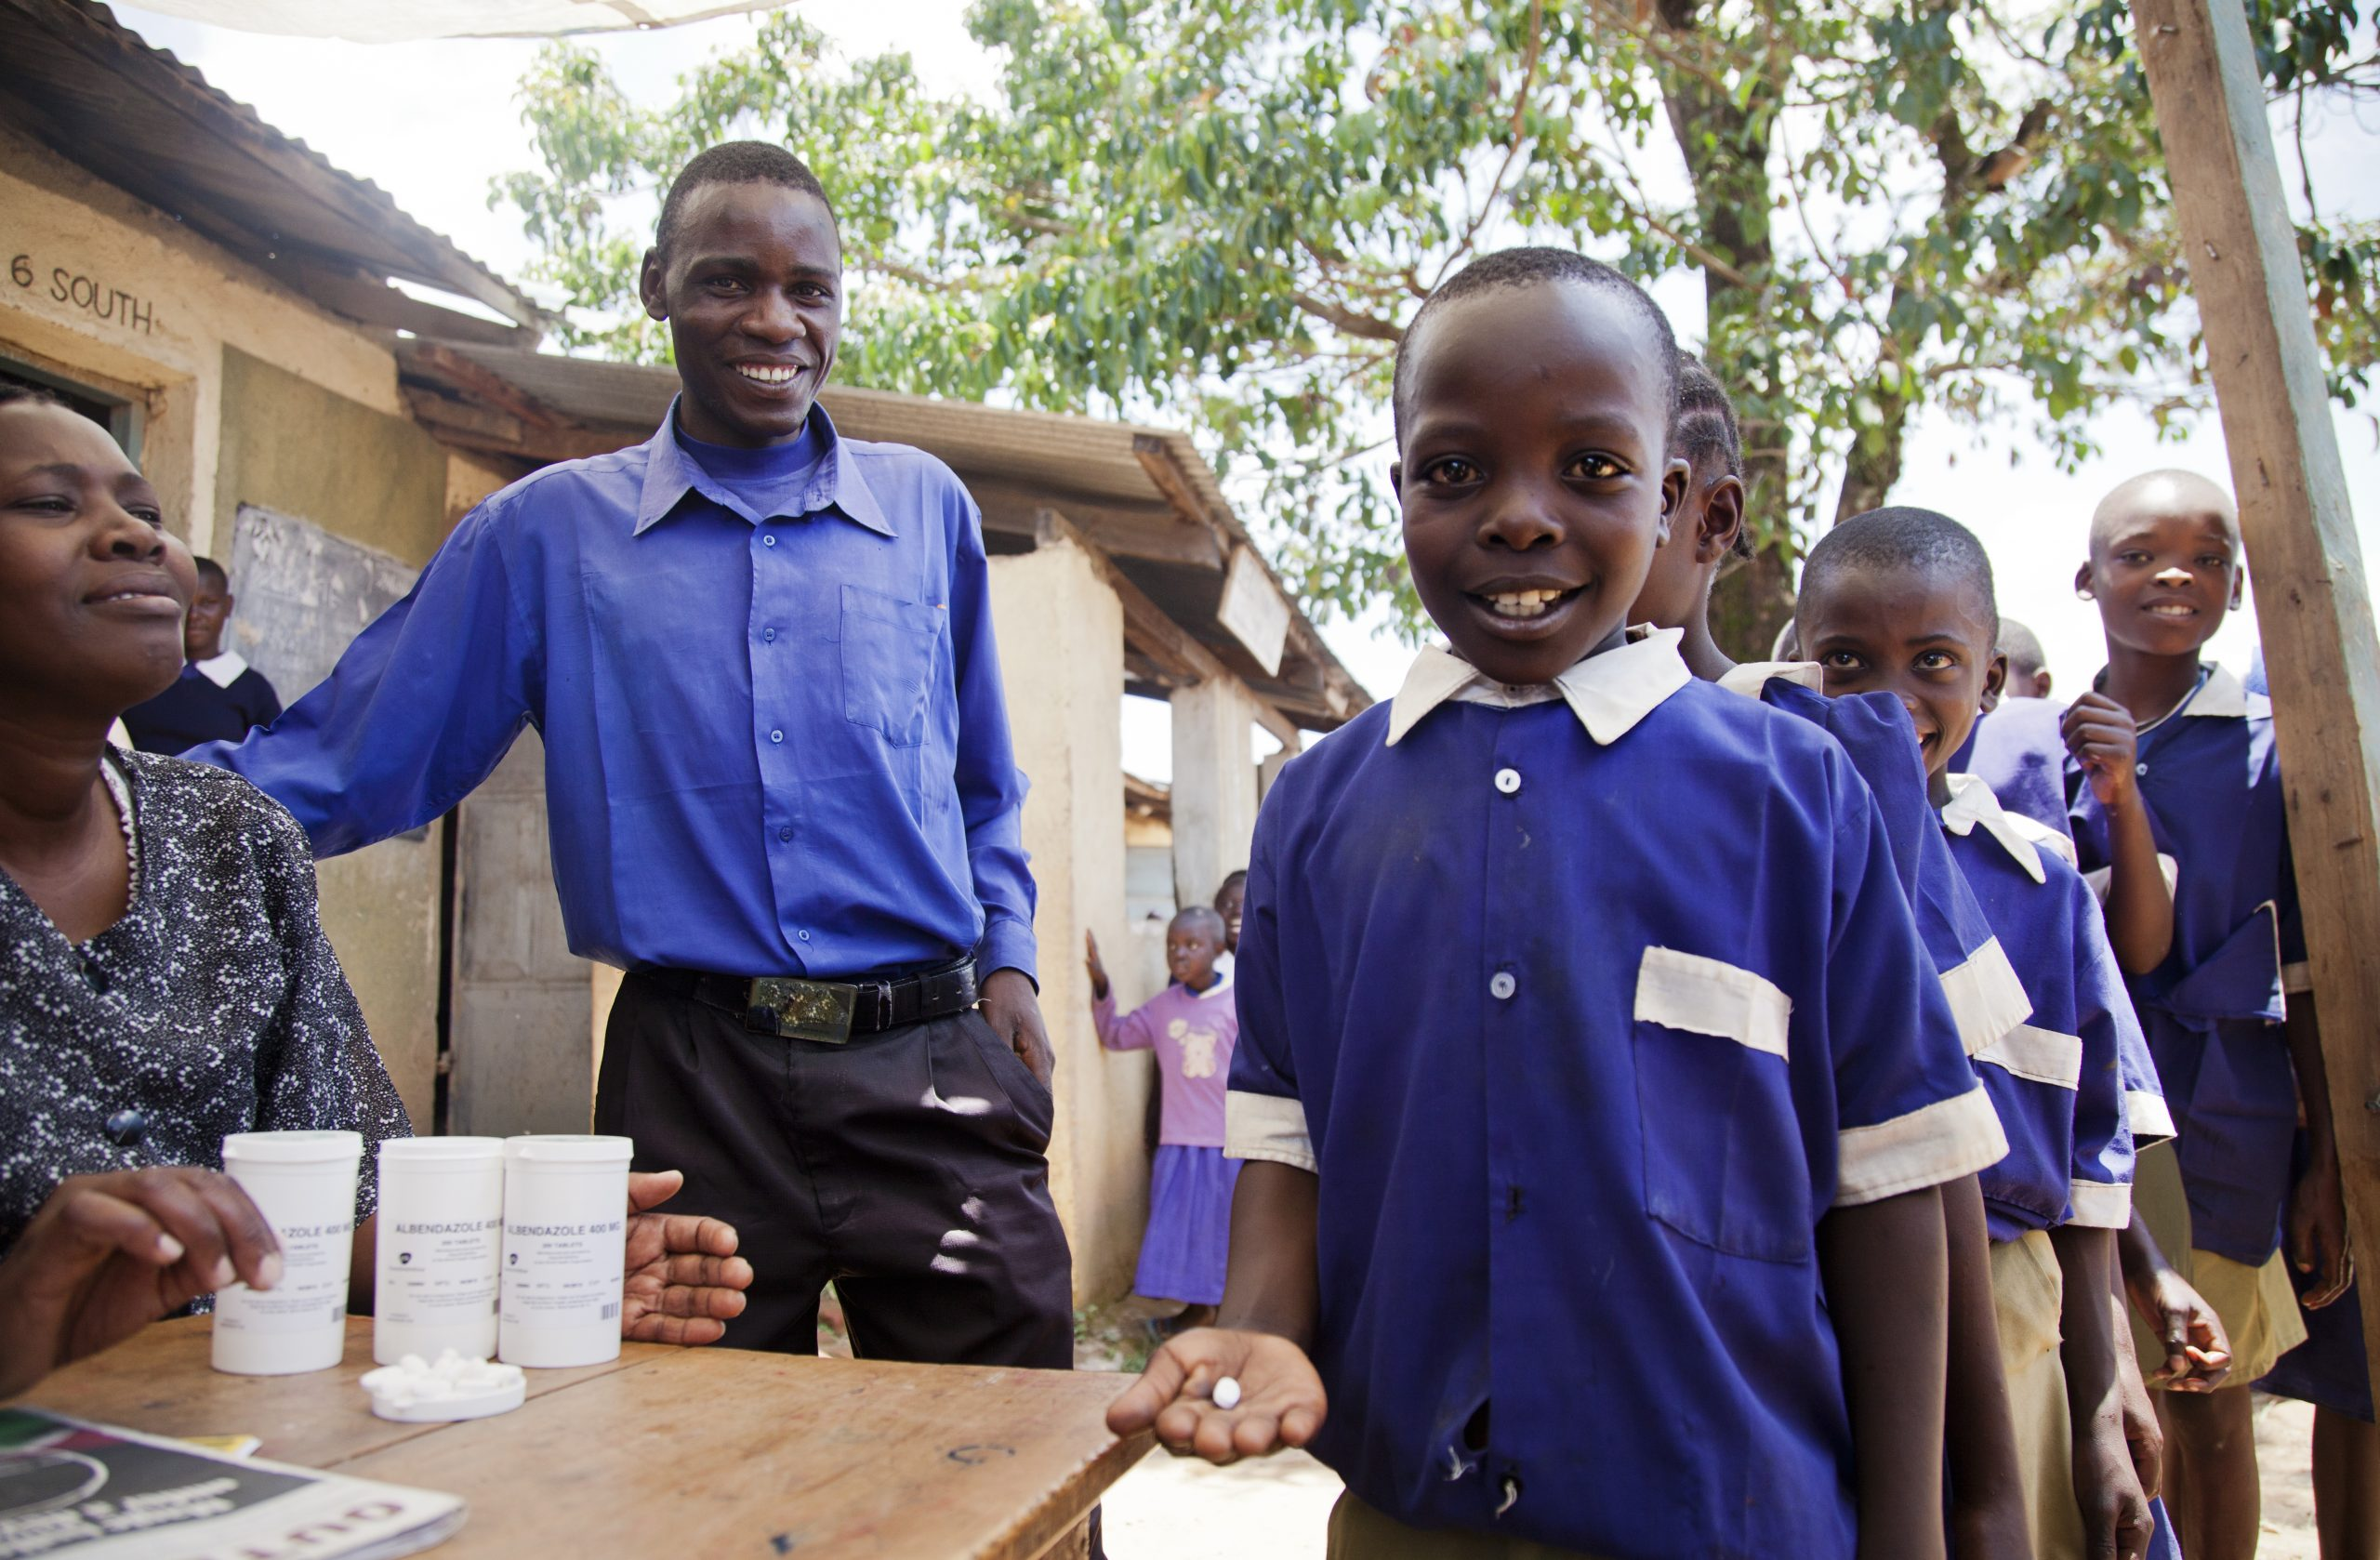
\includegraphics[keepaspectratio,height=3.6cm]{photos/Kenya-Deworm-the-World-Stephanie-Skinner.jpg}};
	\node [gray,anchor=north] at (photo.south) {\tiny{photo:  Stephanie Skinner / Deworm the World}};
	
	\pgfmathsetmacro\xshift{0cm};
	\pgfmathsetmacro\yshift{1.25cm};
	%	\pgfmathsetmacro\mycolor{"gray"};
	
	%\node[anchor=north west,align=left,text width = 9.5cm,xshift=\xshift,yshift=\yshift] (text1) at (0,0) {\textbf{School interventions in Busia, Kenya}};
	
	\node[anchor=north west,align=left,text width = 9.5cm,xshift=\xshift,yshift=\yshift] (text2) at (0.5,0) {\textcolor{structure}{$\bullet$} Michael Kremer convinces NGO to randomize interventions};	
	
	\node[anchor=north west,align=left,text width = 9.5cm,xshift=\xshift,yshift=\yshift] (text3) at (0.5,-0.625) {\textcolor{structure}{$\bullet$} Study of deworming (w/ Miguel) launches RCT movement};
	
	%\node[anchor=north west,align=left,text width = 9.5cm,xshift=\xshift,yshift=\yshift] (text3) at (0.5,-1.875) {\textcolor{structure}{$\bullet$} RCT on flip charts w/ Glewwe, Moulin, \& Zitzewitz)};
	

	
	\end{tikzpicture}
\end{center}

\end{frame}


%%%%%%%%%%%%%%%%%%%%%%%%%%%%%%%%%%%%%%%%%%%%%%%%%%%%%%%%%%%%%%%%%%%%%

\begin{frame}{RCTs in Development Economics:  Trends}

\medskip

\begin{center}
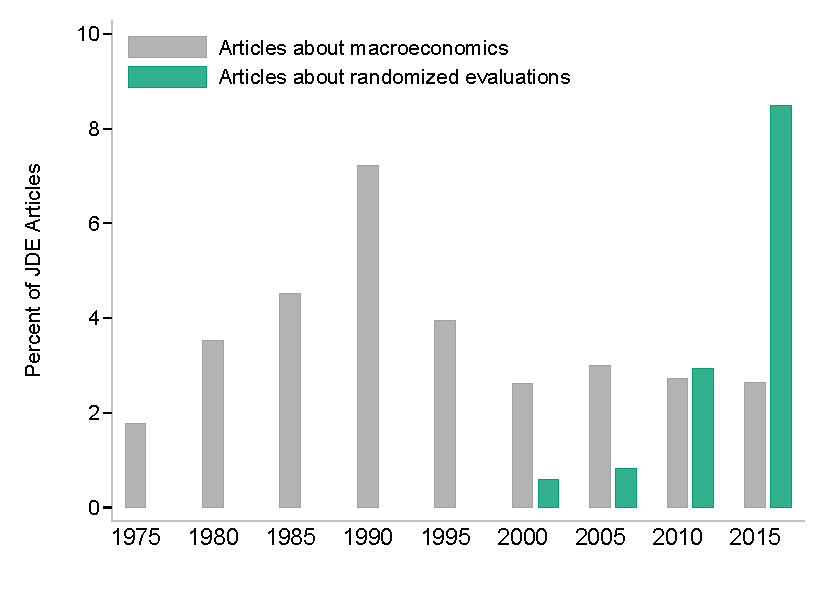
\includegraphics[width=0.64\textwidth]{fig/jde-hist1.pdf}
\end{center}

%\medskip
Abstracts of 2,695 \textit{Journal of Development Economics} articles \\
(all articles published prior to 2019, starting form Volume 1 in 1974)


\end{frame}


%%%%%%%%%%%%%%%%%%%%%%%%%%%%%%%%%%%%%%%%%%%%%%%%%%%%%%%%%%%%%%%%%%%%%%%%%%%%%%%%%

\newpage
\begin{frame}{RCTs in Development Economics}

\medskip

\begin{center}
	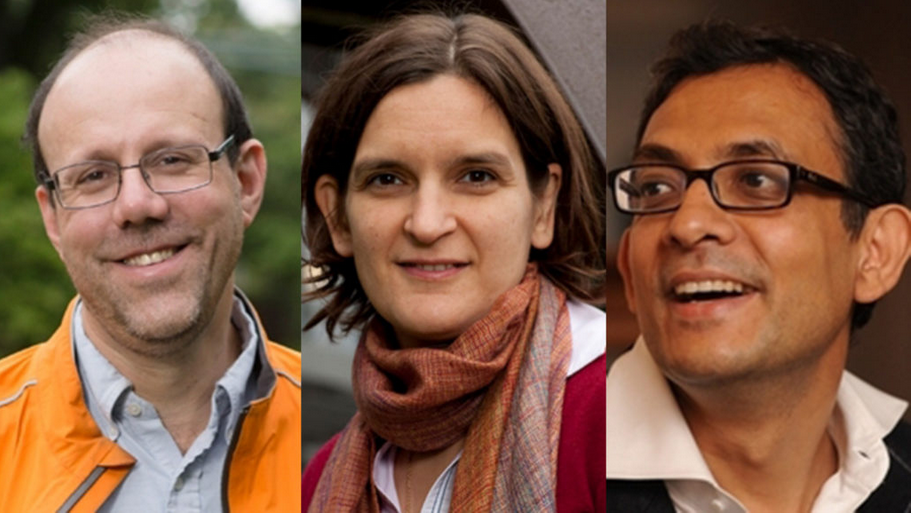
\includegraphics[width=0.72\textwidth]{photos/nobel.png}
\end{center}

\medskip
In 2019, Michael Kremer, Esther Duflo, and Abhijit Banerjee won \\
the Nobel Prize in economics for their promotion of RCTs and\\
their ``experimental approach to alleviating global poverty''


\end{frame}


%%%%%%%%%%%%%%%%%%%%%%%%%%%%%%%%%%%%%%%%%%%%%%%%%%%%%%%%%%%%%%%%%%%%%%%%%%%%

%\begin{frame}<handout:0>[bg,plain]
\begin{frame}[plain]
%\only<beamer>{\begin{adjustwidth}{0cm}{-4cm}}
\begin{center}
	
	\Large{\textcolor{williams}{Regression Analysis of RCTs}}
	
\end{center}
%\only<beamer>{\end{adjustwidth}}
\end{frame}


%%%%%%%%%%%%%%%%%%%%%%%%%%%%%%%%%%%%%%%%%%%%%%%%%%%%%%%%%%%%%%%%%%%%%

\begin{frame}<handout:0>{Treatment Effects Under Random Assignment}

\begin{center}
	\begin{tikzpicture}
	
	% blank canvas
	\only<handout>{\fill[fill=white,draw=white,ultra thin]
		(0,0) -- (11,0) -- (11,6) -- (0,6) -- cycle;}
	\only<beamer>{\fill[fill=white,draw=white,ultra thin]
		(0,0) -- (14,0) -- (14,6) -- (0,6) -- cycle;}
	\only<beamer>{\draw[draw=oiblue!60,fill=oiblue!10,opacity=0.5] (11,1) rectangle (14,5);}
	%\draw[step=1.0,gray!20,thin] (0,0) grid (11,6);
	
	%\node [anchor=north] (photo) at (5,5.875) {\includegraphics[keepaspectratio,height=3.6cm]{photos/Kenya-Deworm-the-World-Stephanie-Skinner.jpg}};
	
	\pgfmathsetmacro\xshift{0.5cm};
	\pgfmathsetmacro\yshift{5.75cm};
	%	\pgfmathsetmacro\mycolor{"gray"};
	
	\node[anchor=north west,align=left,text width = 9.5cm,xshift=\xshift,yshift=\yshift] (text1) at (0,0) {Expected value of control group mean:};	
	
	\node[anchor=north west,align=left,text width = 9.5cm,xshift=\xshift,yshift=\yshift] (text2) at (0.5,-0.75) {$E [ \bar{Y}_{C}]  \ \textcolor{black}{= E [ Y_{i} \vert D_i = 0 ]} \ \textcolor{white}{= E [ Y_{0,i} \vert D_i = 0 ]} \ \textcolor{white}{= E [ Y_{0,i} ]}$};
	
	
	\end{tikzpicture}
\end{center}

\end{frame}



%%%%%%%%%%%%%%%%%%%%%%%%%%%%%%%%%%%%%%%%%%%%%%%%%%%%%%%%%%%%%%%%%%%%%

\begin{frame}<handout:0>{Treatment Effects Under Random Assignment}

\begin{center}
	\begin{tikzpicture}
	
	% blank canvas
	\only<handout>{\fill[fill=white,draw=white,ultra thin]
		(0,0) -- (11,0) -- (11,6) -- (0,6) -- cycle;}
	\only<beamer>{\fill[fill=white,draw=white,ultra thin]
		(0,0) -- (14,0) -- (14,6) -- (0,6) -- cycle;}
	\only<beamer>{\draw[draw=oiblue!60,fill=oiblue!10,opacity=0.5] (11,1) rectangle (14,5);}
	%\draw[step=1.0,gray!20,thin] (0,0) grid (11,6);
	
	%\node [anchor=north] (photo) at (5,5.875) {\includegraphics[keepaspectratio,height=3.6cm]{photos/Kenya-Deworm-the-World-Stephanie-Skinner.jpg}};
	
	\pgfmathsetmacro\xshift{0.5cm};
	\pgfmathsetmacro\yshift{5.75cm};
	%	\pgfmathsetmacro\mycolor{"gray"};
	
	\node[anchor=north west,align=left,text width = 9.5cm,xshift=\xshift,yshift=\yshift] (text1) at (0,0) {Expected value of control group mean:};	
	
	\node[anchor=north west,align=left,text width = 9.5cm,xshift=\xshift,yshift=\yshift] (text2) at (0.5,-0.75) {$E [ \bar{Y}_{C}]  \ \textcolor{black}{= E [ Y_{i} \vert D_i = 0 ]} \ \textcolor{red}{= E [ Y_{0,i} \vert D_i = 0 ]} \ \textcolor{white}{= E [ Y_{0,i} ]}$};
	
	
	\end{tikzpicture}
\end{center}

\end{frame}


%%%%%%%%%%%%%%%%%%%%%%%%%%%%%%%%%%%%%%%%%%%%%%%%%%%%%%%%%%%%%%%%%%%%%

\begin{frame}{Treatment Effects Under Random Assignment}

\begin{center}
	\begin{tikzpicture}
	
	% blank canvas
	\only<handout>{\fill[fill=white,draw=white,ultra thin]
		(0,0) -- (11,0) -- (11,6) -- (0,6) -- cycle;}
	\only<beamer>{\fill[fill=white,draw=white,ultra thin]
		(0,0) -- (14,0) -- (14,6) -- (0,6) -- cycle;}
	\only<beamer>{\draw[draw=oiblue!60,fill=oiblue!10,opacity=0.5] (11,1) rectangle (14,5);}
	%\draw[step=1.0,gray!20,thin] (0,0) grid (11,6);
	
	%\node [anchor=north] (photo) at (5,5.875) {\includegraphics[keepaspectratio,height=3.6cm]{photos/Kenya-Deworm-the-World-Stephanie-Skinner.jpg}};
	
	\pgfmathsetmacro\xshift{0.5cm};
	\pgfmathsetmacro\yshift{5.75cm};
	%	\pgfmathsetmacro\mycolor{"gray"};
	
	\node[anchor=north west,align=left,text width = 9.5cm,xshift=\xshift,yshift=\yshift] (text1) at (0,0) {Expected value of control group mean:};	
	
	\node[anchor=north west,align=left,xshift=\xshift,yshift=\yshift] (text2) at (0.5,-0.75) {$E [ \bar{Y}_{C}]  \ \textcolor{black}{= E [ Y_{i} \vert D_i = 0 ]} \ \textcolor{black}{= E [ Y_{0,i} \vert D_i = 0 ]} \ \textcolor{red}{= E [ Y_{0,i} ]}$};
		
	\node[red,anchor=north,align=center,text width = 6cm] (lbl2) at ([xshift=-0.625cm,yshift=-1cm]text2.south east) {equal to population mean because control group is a random sample};	
	\draw[red,->] (lbl2.north) -- ([xshift=-0.625cm]text2.south east);
	
	\end{tikzpicture}
\end{center}

\end{frame}


%%%%%%%%%%%%%%%%%%%%%%%%%%%%%%%%%%%%%%%%%%%%%%%%%%%%%%%%%%%%%%%%%%%%%

\begin{frame}<handout:0>{Treatment Effects Under Random Assignment}

\begin{center}
	\begin{tikzpicture}
	
	% blank canvas
	\only<handout>{\fill[fill=white,draw=white,ultra thin]
		(0,0) -- (11,0) -- (11,6) -- (0,6) -- cycle;}
	\only<beamer>{\fill[fill=white,draw=white,ultra thin]
		(0,0) -- (14,0) -- (14,6) -- (0,6) -- cycle;}
	\only<beamer>{\draw[draw=oiblue!60,fill=oiblue!10,opacity=0.5] (11,1) rectangle (14,5);}
	%\draw[step=1.0,gray!20,thin] (0,0) grid (11,6);
	
	%\node [anchor=north] (photo) at (5,5.875) {\includegraphics[keepaspectratio,height=3.6cm]{photos/Kenya-Deworm-the-World-Stephanie-Skinner.jpg}};
	
	\pgfmathsetmacro\xshift{0.5cm};
	\pgfmathsetmacro\yshift{5.75cm};
	%	\pgfmathsetmacro\mycolor{"gray"};
	
	\node[gray,anchor=north west,align=left,text width = 9.5cm,xshift=\xshift,yshift=\yshift] (text1) at (0,0) {Expected value of control group mean:};	
	
	\node[gray,anchor=north west,align=left,xshift=\xshift,yshift=\yshift] (text2) at (0.5,-0.75) {$E [ \bar{Y}_{C}]  \ \textcolor{gray}{= E [ Y_{i} \vert D_i = 0 ]} \ \textcolor{gray}{= E [ Y_{0,i} \vert D_i = 0 ]} \ \textcolor{gray}{= E [ Y_{0,i} ]}$};
	
	\node[red,anchor=north,align=center,text width = 9.5cm,xshift=\xshift,yshift=\yshift] (text3) at (5,-2) {For those randomly assigned to treatment:};	
	\node[red,anchor=north,align=center,xshift=\xshift,yshift=\yshift] (text4) at (5,-2.75) {$Y_i = \textcolor{white}{\underbrace{ \textcolor{red}{Y_{1,i}} \textcolor{white}{\ - \  Y_{0,i}} }_{\ }  \  \textcolor{white}{+} \  \textcolor{white}{Y_{0,i}}   } $};	
	
	\end{tikzpicture}
\end{center}

\end{frame}



%%%%%%%%%%%%%%%%%%%%%%%%%%%%%%%%%%%%%%%%%%%%%%%%%%%%%%%%%%%%%%%%%%%%%

\begin{frame}<handout:0>{Treatment Effects Under Random Assignment}

\begin{center}
	\begin{tikzpicture}
	
	% blank canvas
	\only<handout>{\fill[fill=white,draw=white,ultra thin]
		(0,0) -- (11,0) -- (11,6) -- (0,6) -- cycle;}
	\only<beamer>{\fill[fill=white,draw=white,ultra thin]
		(0,0) -- (14,0) -- (14,6) -- (0,6) -- cycle;}
	\only<beamer>{\draw[draw=oiblue!60,fill=oiblue!10,opacity=0.5] (11,1) rectangle (14,5);}
	%\draw[step=1.0,gray!20,thin] (0,0) grid (11,6);
	
	%\node [anchor=north] (photo) at (5,5.875) {\includegraphics[keepaspectratio,height=3.6cm]{photos/Kenya-Deworm-the-World-Stephanie-Skinner.jpg}};
	
	\pgfmathsetmacro\xshift{0.5cm};
	\pgfmathsetmacro\yshift{5.75cm};
	%	\pgfmathsetmacro\mycolor{"gray"};
	
	\node[gray,anchor=north west,align=left,text width = 9.5cm,xshift=\xshift,yshift=\yshift] (text1) at (0,0) {Expected value of control group mean:};	
	
	\node[gray,anchor=north west,align=left,xshift=\xshift,yshift=\yshift] (text2) at (0.5,-0.75) {$E [ \bar{Y}_{C}]  \ \textcolor{gray}{= E [ Y_{i} \vert D_i = 0 ]} \ \textcolor{gray}{= E [ Y_{0,i} \vert D_i = 0 ]} \ \textcolor{gray}{= E [ Y_{0,i} ]}$};
	
	\node[anchor=north,align=center,text width = 9.5cm,xshift=\xshift,yshift=\yshift] (text3) at (5,-2) {For those randomly assigned to treatment:};	
	\node[anchor=north,align=center,xshift=\xshift,yshift=\yshift] (text4) at (5,-2.75) {$Y_i = \textcolor{white}{\underbrace{ \textcolor{black}{Y_{1,i}} \textcolor{red}{\ - \  Y_{0,i}} }_{\ }  \  \textcolor{red}{+} \  \textcolor{red}{Y_{0,i}}   } $};	
	
	\end{tikzpicture}
\end{center}

\end{frame}


%%%%%%%%%%%%%%%%%%%%%%%%%%%%%%%%%%%%%%%%%%%%%%%%%%%%%%%%%%%%%%%%%%%%%

\begin{frame}<handout:0>{Treatment Effects Under Random Assignment}

\begin{center}
	\begin{tikzpicture}
	
	% blank canvas
	\only<handout>{\fill[fill=white,draw=white,ultra thin]
		(0,0) -- (11,0) -- (11,6) -- (0,6) -- cycle;}
	\only<beamer>{\fill[fill=white,draw=white,ultra thin]
		(0,0) -- (14,0) -- (14,6) -- (0,6) -- cycle;}
	\only<beamer>{\draw[draw=oiblue!60,fill=oiblue!10,opacity=0.5] (11,1) rectangle (14,5);}
	%\draw[step=1.0,gray!20,thin] (0,0) grid (11,6);
	
	%\node [anchor=north] (photo) at (5,5.875) {\includegraphics[keepaspectratio,height=3.6cm]{photos/Kenya-Deworm-the-World-Stephanie-Skinner.jpg}};
	
	\pgfmathsetmacro\xshift{0.5cm};
	\pgfmathsetmacro\yshift{5.75cm};
	%	\pgfmathsetmacro\mycolor{"gray"};
	
	\node[gray,anchor=north west,align=left,text width = 9.5cm,xshift=\xshift,yshift=\yshift] (text1) at (0,0) {Expected value of control group mean:};	
	
	\node[gray,anchor=north west,align=left,xshift=\xshift,yshift=\yshift] (text2) at (0.5,-0.75) {$E [ \bar{Y}_{C}] \ \textcolor{gray}{= E [ Y_{i} \vert D_i = 0 ]} \ \textcolor{gray}{= E [ Y_{0,i} \vert D_i = 0 ]} \ \textcolor{gray}{= E [ Y_{0,i} ]}$};
	
	\node[anchor=north,align=center,text width = 9.5cm,xshift=\xshift,yshift=\yshift] (text3) at (5,-2) {For those randomly assigned to treatment:};	
	\node[anchor=north,align=center,xshift=\xshift,yshift=\yshift] (text4) at (5,-2.75) {$Y_i = \textcolor{red}{\underbrace{ \textcolor{red}{Y_{1,i}} \textcolor{red}{\ - \  Y_{0,i}} }_{\ }  \  \textcolor{black}{+} \  \textcolor{black}{Y_{0,i}}   } $};	
	
	\node[red,anchor=north,align=center] (lbl4A) at ([xshift=-0.16cm,yshift=-0.25cm]text4.south) {treatment effect on $i$};	
	\draw[red,->] (lbl4A.north) -- ([xshift=-0.16cm,yshift=0.25cm]text4.south);
	%\node[red,anchor=east,align=right] (lbl4C) at ([xshift=0.1cm,yshift=-0.03cm]lbl4A.west) {$\delta_i = $};
	
	%\node[anchor=north,align=center,text width = 6cm] (lbl4B) at ([xshift=0.5cm,yshift=-1cm]text4.south east) {potential outcome \\ 
%	in the absence of treatment};	
%\draw[->] (lbl4B.north) -- ([xshift=-0.125cm,yshift=0.375cm]text4.south east);

\end{tikzpicture}
\end{center}

\end{frame}



%%%%%%%%%%%%%%%%%%%%%%%%%%%%%%%%%%%%%%%%%%%%%%%%%%%%%%%%%%%%%%%%%%%%%

\begin{frame}<handout:0>{Treatment Effects Under Random Assignment}

\begin{center}
	\begin{tikzpicture}
	
	% blank canvas
	\only<handout>{\fill[fill=white,draw=white,ultra thin]
		(0,0) -- (11,0) -- (11,6) -- (0,6) -- cycle;}
	\only<beamer>{\fill[fill=white,draw=white,ultra thin]
		(0,0) -- (14,0) -- (14,6) -- (0,6) -- cycle;}
	\only<beamer>{\draw[draw=oiblue!60,fill=oiblue!10,opacity=0.5] (11,1) rectangle (14,5);}
	%\draw[step=1.0,gray!20,thin] (0,0) grid (11,6);
	
	%\node [anchor=north] (photo) at (5,5.875) {\includegraphics[keepaspectratio,height=3.6cm]{photos/Kenya-Deworm-the-World-Stephanie-Skinner.jpg}};
	
	\pgfmathsetmacro\xshift{0.5cm};
	\pgfmathsetmacro\yshift{5.75cm};
	%	\pgfmathsetmacro\mycolor{"gray"};
	
	\node[gray,anchor=north west,align=left,text width = 9.5cm,xshift=\xshift,yshift=\yshift] (text1) at (0,0) {Expected value of control group mean:};	
	
	\node[gray,anchor=north west,align=left,xshift=\xshift,yshift=\yshift] (text2) at (0.5,-0.75) {$E [ \bar{Y}_{C}] \ \textcolor{gray}{= E [ Y_{i} \vert D_i = 0 ]} \ \textcolor{gray}{= E [ Y_{0,i} \vert D_i = 0 ]} \ \textcolor{gray}{= E [ Y_{0,i} ]}$};
	
	\node[anchor=north,align=center,text width = 9.5cm,xshift=\xshift,yshift=\yshift] (text3) at (5,-2) {For those randomly assigned to treatment:};	
	\node[anchor=north,align=center,xshift=\xshift,yshift=\yshift] (text4) at (5,-2.75) {$Y_i = \textcolor{red}{\underbrace{ \textcolor{red}{Y_{1,i}} \textcolor{red}{\ - \  Y_{0,i}} }_{\ }  \  \textcolor{black}{+} \  \textcolor{black}{Y_{0,i}}   } $};	
	
	\node[red,anchor=north,align=center] (lbl4A) at ([xshift=-0.16cm,yshift=-0.25cm]text4.south) {treatment effect on $i$};	
	\draw[red,->] (lbl4A.north) -- ([xshift=-0.16cm,yshift=0.25cm]text4.south);
	\node[red,anchor=east,align=right] (lbl4C) at ([xshift=0.1cm,yshift=-0.03cm]lbl4A.west) {$\delta_i = $};
	
	%\node[anchor=north,align=center,text width = 6cm] (lbl4B) at ([xshift=0.5cm,yshift=-1cm]text4.south east) {potential outcome \\ 
	%	in the absence of treatment};	
	%\draw[->] (lbl4B.north) -- ([xshift=-0.125cm,yshift=0.375cm]text4.south east);
	
	\end{tikzpicture}
\end{center}

\end{frame}



%%%%%%%%%%%%%%%%%%%%%%%%%%%%%%%%%%%%%%%%%%%%%%%%%%%%%%%%%%%%%%%%%%%%%

\begin{frame}<handout:0>{Treatment Effects Under Random Assignment}

\begin{center}
	\begin{tikzpicture}
	
	% blank canvas
	\only<handout>{\fill[fill=white,draw=white,ultra thin]
		(0,0) -- (11,0) -- (11,6) -- (0,6) -- cycle;}
	\only<beamer>{\fill[fill=white,draw=white,ultra thin]
		(0,0) -- (14,0) -- (14,6) -- (0,6) -- cycle;}
	\only<beamer>{\draw[draw=oiblue!60,fill=oiblue!10,opacity=0.5] (11,1) rectangle (14,5);}
	%\draw[step=1.0,gray!20,thin] (0,0) grid (11,6);
	
	%\node [anchor=north] (photo) at (5,5.875) {\includegraphics[keepaspectratio,height=3.6cm]{photos/Kenya-Deworm-the-World-Stephanie-Skinner.jpg}};
	
	\pgfmathsetmacro\xshift{0.5cm};
	\pgfmathsetmacro\yshift{5.75cm};
	%	\pgfmathsetmacro\mycolor{"gray"};
	
	\node[gray,anchor=north west,align=left,text width = 9.5cm,xshift=\xshift,yshift=\yshift] (text1) at (0,0) {Expected value of control group mean:};	
	
	\node[gray,anchor=north west,align=left,xshift=\xshift,yshift=\yshift] (text2) at (0.5,-0.75) {$E [ \bar{Y}_{C}] \ \textcolor{gray}{= E [ Y_{i} \vert D_i = 0 ]} \ \textcolor{gray}{= E [ Y_{0,i} \vert D_i = 0 ]} \ \textcolor{gray}{= E [ Y_{0,i} ]}$};
	
	\node[anchor=north,align=center,text width = 9.5cm,xshift=\xshift,yshift=\yshift] (text3) at (5,-2) {For those randomly assigned to treatment:};	
	\node[anchor=north,align=center,xshift=\xshift,yshift=\yshift] (text4) at (5,-2.75) {$Y_i = \textcolor{red}{\underbrace{ \textcolor{red}{Y_{1,i}} \textcolor{red}{\ - \  Y_{0,i}} }_{\ }  \  \textcolor{black}{+} \  \textcolor{black}{Y_{0,i}}   } $};	
	
	\node[red,anchor=north,align=center] (lbl4A) at ([xshift=-0.16cm,yshift=-0.25cm]text4.south) {treatment effect on $i$};	
	\draw[red,->] (lbl4A.north) -- ([xshift=-0.16cm,yshift=0.25cm]text4.south);
	\node[red,anchor=east,align=right] (lbl4C) at ([xshift=0.1cm,yshift=-0.03cm]lbl4A.west) {$\delta_i = $};
	
	\node[anchor=north,align=center,text width = 6cm] (lbl4B) at ([xshift=0.5cm,yshift=-1cm]text4.south east) {potential outcome \\ 
									in the absence of treatment};	
	\draw[->] (lbl4B.north) -- ([xshift=-0.125cm,yshift=0.375cm]text4.south east);
	
	\end{tikzpicture}
\end{center}

\end{frame}






%%%%%%%%%%%%%%%%%%%%%%%%%%%%%%%%%%%%%%%%%%%%%%%%%%%%%%%%%%%%%%%%%%%%%

\begin{frame}<handout:0>{Treatment Effects Under Random Assignment}

\begin{center}
	\begin{tikzpicture}
	
	% blank canvas
	\only<handout>{\fill[fill=white,draw=white,ultra thin]
		(0,0) -- (11,0) -- (11,6) -- (0,6) -- cycle;}
	\only<beamer>{\fill[fill=white,draw=white,ultra thin]
		(0,0) -- (14,0) -- (14,6) -- (0,6) -- cycle;}
	\only<beamer>{\draw[draw=oiblue!60,fill=oiblue!10,opacity=0.5] (11,1) rectangle (14,5);}
	%\draw[step=1.0,gray!20,thin] (0,0) grid (11,6);
	
	%\node [anchor=north] (photo) at (5,5.875) {\includegraphics[keepaspectratio,height=3.6cm]{photos/Kenya-Deworm-the-World-Stephanie-Skinner.jpg}};
	
	\pgfmathsetmacro\xshift{0.5cm};
	\pgfmathsetmacro\yshift{5.75cm};
	%	\pgfmathsetmacro\mycolor{"gray"};
	
	\node[gray,anchor=north west,align=left,text width = 9.5cm,xshift=\xshift,yshift=\yshift] (text1) at (0,0) {Expected value of control group mean:};	
	
	\node[gray,anchor=north west,align=left,xshift=\xshift,yshift=\yshift] (text2) at (0.5,-0.75) {$E [ \bar{Y}_{C}]  \ \textcolor{gray}{= E [ Y_{i} \vert D_i = 0 ]} \ \textcolor{gray}{= E [ Y_{0,i} \vert D_i = 0 ]} \ \textcolor{gray}{= E [ Y_{0,i} ]}$};
	
	\node[anchor=north west,align=left,text width = 9.5cm,xshift=\xshift,yshift=\yshift] (text3) at (0,-1.75) {Expected value of treatment group mean:};	

	\node[anchor=north west,align=left,xshift=\xshift,yshift=\yshift] (text4) at (0.5,-2.5) {$E [ \bar{Y}_{T}] \ \textcolor{black}{= E [ Y_{i} \vert D_i = 1 ]}  \ \textcolor{black}{= E [ Y_{1,i} \vert D_i = 1 ]} $};
	

	
	\end{tikzpicture}
\end{center}

\end{frame}



%%%%%%%%%%%%%%%%%%%%%%%%%%%%%%%%%%%%%%%%%%%%%%%%%%%%%%%%%%%%%%%%%%%%%

\begin{frame}<handout:0>{Treatment Effects Under Random Assignment}

\begin{center}
	\begin{tikzpicture}
	
	% blank canvas
	\only<handout>{\fill[fill=white,draw=white,ultra thin]
		(0,0) -- (11,0) -- (11,6) -- (0,6) -- cycle;}
	\only<beamer>{\fill[fill=white,draw=white,ultra thin]
		(0,0) -- (14,0) -- (14,6) -- (0,6) -- cycle;}
	\only<beamer>{\draw[draw=oiblue!60,fill=oiblue!10,opacity=0.5] (11,1) rectangle (14,5);}
	%\draw[step=1.0,gray!20,thin] (0,0) grid (11,6);
	
	%\node [anchor=north] (photo) at (5,5.875) {\includegraphics[keepaspectratio,height=3.6cm]{photos/Kenya-Deworm-the-World-Stephanie-Skinner.jpg}};
	
	\pgfmathsetmacro\xshift{0.5cm};
	\pgfmathsetmacro\yshift{5.75cm};
	%	\pgfmathsetmacro\mycolor{"gray"};
	
	\node[gray,anchor=north west,align=left,text width = 9.5cm,xshift=\xshift,yshift=\yshift] (text1) at (0,0) {Expected value of control group mean:};	
	
	\node[gray,anchor=north west,align=left,xshift=\xshift,yshift=\yshift] (text2) at (0.5,-0.75) {$E [ \bar{Y}_{C}]  \ \textcolor{gray}{= E [ Y_{i} \vert D_i = 0 ]} \ \textcolor{gray}{= E [ Y_{0,i} \vert D_i = 0 ]} \ \textcolor{gray}{= E [ Y_{0,i} ]}$};
	
	\node[anchor=north west,align=left,text width = 9.5cm,xshift=\xshift,yshift=\yshift] (text3) at (0,-1.75) {Expected value of treatment group mean:};	
	
	\node[anchor=north west,align=left,xshift=\xshift,yshift=\yshift] (text4) at (0.5,-2.5) {$E [ \bar{Y}_{T}] \ \textcolor{black}{= E [ Y_{i} \vert D_i = 1 ]}  \ \textcolor{black}{= E [ Y_{1,i} \vert D_i = 1 ]}$};
	\node[white,anchor=north west,align=left,xshift=\xshift,yshift=\yshift] (text5) at (0.5,-3.125) {$E [ \bar{Y}_{T}] \ \textcolor{white}{= E [ Y_{i} \vert D_i = 1 ]}  \ \textcolor{red}{= E [ \delta_i + Y_{0,i} \vert D_i = 1 ]}$};	
	
	
	\end{tikzpicture}
\end{center}

\end{frame}


%%%%%%%%%%%%%%%%%%%%%%%%%%%%%%%%%%%%%%%%%%%%%%%%%%%%%%%%%%%%%%%%%%%%%

\begin{frame}<handout:0>{Treatment Effects Under Random Assignment}

\begin{center}
	\begin{tikzpicture}
	
	% blank canvas
	\only<handout>{\fill[fill=white,draw=white,ultra thin]
		(0,0) -- (11,0) -- (11,6) -- (0,6) -- cycle;}
	\only<beamer>{\fill[fill=white,draw=white,ultra thin]
		(0,0) -- (14,0) -- (14,6) -- (0,6) -- cycle;}
	\only<beamer>{\draw[draw=oiblue!60,fill=oiblue!10,opacity=0.5] (11,1) rectangle (14,5);}
	%\draw[step=1.0,gray!20,thin] (0,0) grid (11,6);
	
	%\node [anchor=north] (photo) at (5,5.875) {\includegraphics[keepaspectratio,height=3.6cm]{photos/Kenya-Deworm-the-World-Stephanie-Skinner.jpg}};
	
	\pgfmathsetmacro\xshift{0.5cm};
	\pgfmathsetmacro\yshift{5.75cm};
	%	\pgfmathsetmacro\mycolor{"gray"};
	
	\node[gray,anchor=north west,align=left,text width = 9.5cm,xshift=\xshift,yshift=\yshift] (text1) at (0,0) {Expected value of control group mean:};	
	
	\node[gray,anchor=north west,align=left,xshift=\xshift,yshift=\yshift] (text2) at (0.5,-0.75) {$E [ \bar{Y}_{C}]  \ \textcolor{gray}{= E [ Y_{i} \vert D_i = 0 ]} \ \textcolor{gray}{= E [ Y_{0,i} \vert D_i = 0 ]} \ \textcolor{gray}{= E [ Y_{0,i} ]}$};
	
	\node[anchor=north west,align=left,text width = 9.5cm,xshift=\xshift,yshift=\yshift] (text3) at (0,-1.75) {Expected value of treatment group mean:};	
	
	\node[anchor=north west,align=left,xshift=\xshift,yshift=\yshift] (text4) at (0.5,-2.5) {$E [ \bar{Y}_{T}] \ \textcolor{black}{= E [ Y_{i} \vert D_i = 1 ]}  \ \textcolor{black}{= E [ Y_{1,i} \vert D_i = 1 ]}$};
	\node[white,anchor=north west,align=left,xshift=\xshift,yshift=\yshift] (text5) at (0.5,-3.125) {$E [ \bar{Y}_{T}] \ \textcolor{white}{= E [ Y_{i} \vert D_i = 1 ]}  \ \textcolor{black}{= E [ \delta_i + Y_{0,i} \vert D_i = 1 ]}$};	
	\node[white,anchor=north west,align=left,xshift=\xshift,yshift=\yshift] (text6) at (0.5,-3.75) {$E [ \bar{Y}_{T}] \ \textcolor{white}{= E [ Y_{i} \vert D_i = 1 ]}  \ \textcolor{red}{= E [ \delta_i  \vert D_i = 1  ] + E [ Y_{0,i} \vert D_i = 1 ]}$};
	
	
	\end{tikzpicture}
\end{center}

\end{frame}


%%%%%%%%%%%%%%%%%%%%%%%%%%%%%%%%%%%%%%%%%%%%%%%%%%%%%%%%%%%%%%%%%%%%%

\begin{frame}{Treatment Effects Under Random Assignment}

\begin{center}
	\begin{tikzpicture}
	
	% blank canvas
	\only<handout>{\fill[fill=white,draw=white,ultra thin]
		(0,0) -- (11,0) -- (11,6) -- (0,6) -- cycle;}
	\only<beamer>{\fill[fill=white,draw=white,ultra thin]
		(0,0) -- (14,0) -- (14,6) -- (0,6) -- cycle;}
	\only<beamer>{\draw[draw=oiblue!60,fill=oiblue!10,opacity=0.5] (11,1) rectangle (14,5);}
	%\draw[step=1.0,gray!20,thin] (0,0) grid (11,6);
	
	%\node [anchor=north] (photo) at (5,5.875) {\includegraphics[keepaspectratio,height=3.6cm]{photos/Kenya-Deworm-the-World-Stephanie-Skinner.jpg}};
	
	\pgfmathsetmacro\xshift{0.5cm};
	\pgfmathsetmacro\yshift{5.75cm};
	%	\pgfmathsetmacro\mycolor{"gray"};
	
	\node[gray,anchor=north west,align=left,text width = 9.5cm,xshift=\xshift,yshift=\yshift] (text1) at (0,0) {Expected value of control group mean:};	
	
	\node[gray,anchor=north west,align=left,xshift=\xshift,yshift=\yshift] (text2) at (0.5,-0.75) {$E [ \bar{Y}_{C}]  \ \textcolor{gray}{= E [ Y_{i} \vert D_i = 0 ]} \ \textcolor{gray}{= E [ Y_{0,i} \vert D_i = 0 ]} \ \textcolor{gray}{= E [ Y_{0,i} ]}$};
	
	\node[anchor=north west,align=left,text width = 9.5cm,xshift=\xshift,yshift=\yshift] (text3) at (0,-1.75) {Expected value of treatment group mean:};	
	
	\node[anchor=north west,align=left,xshift=\xshift,yshift=\yshift] (text4) at (0.5,-2.5) {$E [ \bar{Y}_{T}] \ \textcolor{black}{= E [ Y_{i} \vert D_i = 1 ]}  \ \textcolor{black}{= E [ Y_{1,i} \vert D_i = 1 ]}$};
	\node[white,anchor=north west,align=left,xshift=\xshift,yshift=\yshift] (text5) at (0.5,-3.125) {$E [ \bar{Y}_{T}] \ \textcolor{white}{= E [ Y_{i} \vert D_i = 1 ]}  \ \textcolor{black}{= E [ \delta_i + Y_{0,i} \vert D_i = 1 ]}$};	
	\node[white,anchor=north west,align=left,xshift=\xshift,yshift=\yshift] (text6) at (0.5,-3.75) {$E [ \bar{Y}_{T}] \ \textcolor{white}{= E [ Y_{i} \vert D_i = 1 ]}  \ \textcolor{black}{= E [ \delta_i  \vert D_i = 1  ] + E [ Y_{0,i} \vert D_i = 1 ]}$};
	\node[white,anchor=north west,align=left,xshift=\xshift,yshift=\yshift] (text6) at (0.5,-4.375) {$E [ \bar{Y}_{T}] \ \textcolor{white}{= E [ Y_{i} \vert D_i = 1 ]}  \ \textcolor{red}{= \textcolor{red}{E [ \delta_i ]} + \textcolor{red}{E [ Y_{0,i} ]}}$};	
	
	\end{tikzpicture}
\end{center}

\end{frame}



%%%%%%%%%%%%%%%%%%%%%%%%%%%%%%%%%%%%%%%%%%%%%%%%%%%%%%%%%%%%%%%%%%%%%

\begin{frame}<handout:0>{Treatment Effects Under Random Assignment}

\begin{center}
	\begin{tikzpicture}
	
	% blank canvas
	\only<handout>{\fill[fill=white,draw=white,ultra thin]
		(0,0) -- (11,0) -- (11,6) -- (0,6) -- cycle;}
	\only<beamer>{\fill[fill=white,draw=white,ultra thin]
		(0,0) -- (14,0) -- (14,6) -- (0,6) -- cycle;}
	\only<beamer>{\draw[draw=oiblue!60,fill=oiblue!10,opacity=0.5] (11,1) rectangle (14,5);}
	%\draw[step=1.0,gray!20,thin] (0,0) grid (11,6);
	
	%\node [anchor=north] (photo) at (5,5.875) {\includegraphics[keepaspectratio,height=3.6cm]{photos/Kenya-Deworm-the-World-Stephanie-Skinner.jpg}};
	
	\pgfmathsetmacro\xshift{0.5cm};
	\pgfmathsetmacro\yshift{5.75cm};
	%	\pgfmathsetmacro\mycolor{"gray"};
	
	\node[gray,anchor=north west,align=left,text width = 9.5cm,xshift=\xshift,yshift=\yshift] (text1) at (0,0) {Expected value of control group mean:};	
	
	\node[gray,anchor=north west,align=left,xshift=\xshift,yshift=\yshift] (text2) at (0.5,-0.75) {$E [ \bar{Y}_{C}]  \ \textcolor{gray}{= E [ Y_{i} \vert D_i = 0 ]} \ \textcolor{gray}{= E [ Y_{0,i} \vert D_i = 0 ]} \ \textcolor{gray}{= E [ Y_{0,i} ]}$};
	
	\node[anchor=north west,align=left,text width = 9.5cm,xshift=\xshift,yshift=\yshift] (text3) at (0,-1.75) {Expected value of treatment group mean:};	
	
	\node[anchor=north west,align=left,xshift=\xshift,yshift=\yshift] (text4) at (0.5,-2.5) {$E [ \bar{Y}_{T}] \ \textcolor{black}{= E [ Y_{i} \vert D_i = 1 ]}  \ \textcolor{black}{= E [ Y_{1,i} \vert D_i = 1 ]}$};
	\node[white,anchor=north west,align=left,xshift=\xshift,yshift=\yshift] (text5) at (0.5,-3.125) {$E [ \bar{Y}_{T}] \ \textcolor{white}{= E [ Y_{i} \vert D_i = 1 ]}  \ \textcolor{black}{= E [ \delta_i + Y_{0,i} \vert D_i = 1 ]}$};	
	\node[white,anchor=north west,align=left,xshift=\xshift,yshift=\yshift] (text6) at (0.5,-3.75) {$E [ \bar{Y}_{T}] \ \textcolor{white}{= E [ Y_{i} \vert D_i = 1 ]}  \ \textcolor{black}{= E [ \delta_i  \vert D_i = 1  ] + E [ Y_{0,i} \vert D_i = 1 ]}$};
	\node[white,anchor=north west,align=left,xshift=\xshift,yshift=\yshift] (text7) at (0.5,-4.375) {$E [ \bar{Y}_{T}] \ \textcolor{white}{= E [ Y_{i} \vert D_i = 1 ]}  \ \textcolor{black}{= \textcolor{red}{E [ \delta_i ]} + \textcolor{black}{E [ Y_{0,i} ]}}$};	
	
	\node[red,anchor=north] (lbl) at ([xshift=1.25cm,yshift=-0.15cm]text7.south) {average treatment effect};
	\draw[red,->] (lbl.north) -- ([xshift=1.25cm]text7.south);
	
	\end{tikzpicture}
\end{center}

\end{frame}



%%%%%%%%%%%%%%%%%%%%%%%%%%%%%%%%%%%%%%%%%%%%%%%%%%%%%%%%%%%%%%%%%%%%%

\begin{frame}{Treatment Effects Under Random Assignment}

\begin{center}
	\begin{tikzpicture}
	
	% blank canvas
	\only<handout>{\fill[fill=white,draw=white,ultra thin]
		(0,0) -- (11,0) -- (11,6) -- (0,6) -- cycle;}
	\only<beamer>{\fill[fill=white,draw=white,ultra thin]
		(0,0) -- (14,0) -- (14,6) -- (0,6) -- cycle;}
	\only<beamer>{\draw[draw=oiblue!60,fill=oiblue!10,opacity=0.5] (11,1) rectangle (14,5);}
	%\draw[step=1.0,gray!20,thin] (0,0) grid (11,6);
	
	%\node [anchor=north] (photo) at (5,5.875) {\includegraphics[keepaspectratio,height=3.6cm]{photos/Kenya-Deworm-the-World-Stephanie-Skinner.jpg}};
	
	\pgfmathsetmacro\xshift{0.5cm};
	\pgfmathsetmacro\yshift{5.75cm};
	%	\pgfmathsetmacro\mycolor{"gray"};
	
	\node[gray,anchor=north west,align=left,text width = 9.5cm,xshift=\xshift,yshift=\yshift] (text1) at (0,0) {Expected value of control group mean:};	
	
	\node[gray,anchor=north west,align=left,xshift=\xshift,yshift=\yshift] (text2) at (0.5,-0.75) {$E [ \bar{Y}_{C}]  \ \textcolor{gray}{= E [ Y_{i} \vert D_i = 0 ]} \ \textcolor{gray}{= E [ Y_{0,i} \vert D_i = 0 ]} \ \textcolor{red}{= E [ Y_{0,i} ]}$};
	
	\node[anchor=north west,align=left,text width = 9.5cm,xshift=\xshift,yshift=\yshift] (text3) at (0,-1.75) {Expected value of treatment group mean:};	
	
	\node[anchor=north west,align=left,xshift=\xshift,yshift=\yshift] (text4) at (0.5,-2.5) {$E [ \bar{Y}_{T}] \ \textcolor{black}{= E [ Y_{i} \vert D_i = 1 ]}  \ \textcolor{black}{= E [ Y_{1,i} \vert D_i = 1 ]}$};
	\node[white,anchor=north west,align=left,xshift=\xshift,yshift=\yshift] (text5) at (0.5,-3.125) {$E [ \bar{Y}_{T}] \ \textcolor{white}{= E [ Y_{i} \vert D_i = 1 ]}  \ \textcolor{black}{= E [ \delta_i + Y_{0,i} \vert D_i = 1 ]}$};	
	\node[white,anchor=north west,align=left,xshift=\xshift,yshift=\yshift] (text6) at (0.5,-3.75) {$E [ \bar{Y}_{T}] \ \textcolor{white}{= E [ Y_{i} \vert D_i = 1 ]}  \ \textcolor{black}{= E [ \delta_i  \vert D_i = 1  ] + E [ Y_{0,i} \vert D_i = 1 ]}$};
	\node[white,anchor=north west,align=left,xshift=\xshift,yshift=\yshift] (text7) at (0.5,-4.375) {$E [ \bar{Y}_{T}] \ \textcolor{white}{= E [ Y_{i} \vert D_i = 1 ]}  \ \textcolor{black}{= \textcolor{black}{E [ \delta_i ]} + \textcolor{red}{E [ Y_{0,i} ]}}$};	
	
	\node[anchor=north] (lbl) at ([xshift=1.25cm,yshift=-0.15cm]text7.south) {average treatment effect};
	\draw[->] (lbl.north) -- ([xshift=1.25cm]text7.south);
	
	\node[red,anchor=north,align=center,text width=3.6cm] (lbl2) at (9,4) {expected outcome \\
	in absence of treatment};
	\draw[red,->,thick] (lbl2.north) -- (text2.south east);
	\draw[red,->,thick] (lbl2.south) -- (text7.north east);
	
	\end{tikzpicture}
\end{center}

\end{frame}



%%%%%%%%%%%%%%%%%%%%%%%%%%%%%%%%%%%%%%%%%%%%%%%%%%%%%%%%%%%%%%%%%%%%%

\begin{frame}<handout:0>{$H_0$:  $ATE = 0$}

\begin{center}
	\begin{tikzpicture}
	
	% blank canvas
	\only<handout>{\fill[fill=white,draw=white,ultra thin]
		(0,0) -- (11,0) -- (11,6) -- (0,6) -- cycle;}
	\only<beamer>{\fill[fill=white,draw=white,ultra thin]
		(0,0) -- (14,0) -- (14,6) -- (0,6) -- cycle;}
	\only<beamer>{\draw[draw=oiblue!60,fill=oiblue!10,opacity=0.5] (11,1) rectangle (14,5);}
	%\draw[step=1.0,gray!20,thin] (0,0) grid (11,6);
	
	%\node [anchor=north] (photo) at (5,5.875) {\includegraphics[keepaspectratio,height=3.6cm]{photos/Kenya-Deworm-the-World-Stephanie-Skinner.jpg}};
	
	\pgfmathsetmacro\xshift{0.5cm};
	\pgfmathsetmacro\yshift{5.75cm};
	%	\pgfmathsetmacro\mycolor{"gray"};
	
	\node[anchor=north west,align=left,text width = 9.5cm,xshift=\xshift,yshift=\yshift] (text1) at (0,0) {\textbf{Null hypothesis ($H_0$):}};
	\node[anchor=north west,align=left,text width = 9.5cm] (text2) at (text1.south west) {The average treatment effect is zero:  $ATE=0$};	
	%\node[anchor=north west,align=left,text width = 9.5cm] (text3) at (text2.south west) {Or, equivalently:  $\bar{Y}_T = \bar{Y}_C$};	

	
	\end{tikzpicture}
\end{center}

\end{frame}


%%%%%%%%%%%%%%%%%%%%%%%%%%%%%%%%%%%%%%%%%%%%%%%%%%%%%%%%%%%%%%%%%%%%%

\begin{frame}<handout:0>{$H_0$:  $ATE = 0$}

\begin{center}
	\begin{tikzpicture}
	
	% blank canvas
	\only<handout>{\fill[fill=white,draw=white,ultra thin]
		(0,0) -- (11,0) -- (11,6) -- (0,6) -- cycle;}
	\only<beamer>{\fill[fill=white,draw=white,ultra thin]
		(0,0) -- (14,0) -- (14,6) -- (0,6) -- cycle;}
	\only<beamer>{\draw[draw=oiblue!60,fill=oiblue!10,opacity=0.5] (11,1) rectangle (14,5);}
	%\draw[step=1.0,gray!20,thin] (0,0) grid (11,6);
	
	%\node [anchor=north] (photo) at (5,5.875) {\includegraphics[keepaspectratio,height=3.6cm]{photos/Kenya-Deworm-the-World-Stephanie-Skinner.jpg}};
	
	\pgfmathsetmacro\xshift{0.5cm};
	\pgfmathsetmacro\yshift{5.75cm};
	%	\pgfmathsetmacro\mycolor{"gray"};
	
	\node[anchor=north west,align=left,text width = 9.5cm,xshift=\xshift,yshift=\yshift] (text1) at (0,0) {\textbf{Null hypothesis ($H_0$):}};
	\node[anchor=north west,align=left,text width = 9.5cm] (text2) at (text1.south west) {The average treatment effect is zero:  $ATE=0$};	
	\node[anchor=north west,align=left,text width = 9.5cm] (text3) at (text2.south west) {Or, equivalently:  $\bar{Y}_T = \bar{Y}_C$};	
	
	\end{tikzpicture}
\end{center}

\end{frame}


%%%%%%%%%%%%%%%%%%%%%%%%%%%%%%%%%%%%%%%%%%%%%%%%%%%%%%%%%%%%%%%%%%%%%

\begin{frame}<handout:0>{$H_0$:  $ATE = 0$}

\begin{center}
	\begin{tikzpicture}
	
	% blank canvas
	\only<handout>{\fill[fill=white,draw=white,ultra thin]
		(0,0) -- (11,0) -- (11,6) -- (0,6) -- cycle;}
	\only<beamer>{\fill[fill=white,draw=white,ultra thin]
		(0,0) -- (14,0) -- (14,6) -- (0,6) -- cycle;}
	\only<beamer>{\draw[draw=oiblue!60,fill=oiblue!10,opacity=0.5] (11,1) rectangle (14,5);}
	%\draw[step=1.0,gray!20,thin] (0,0) grid (11,6);
	
	%\node [anchor=north] (photo) at (5,5.875) {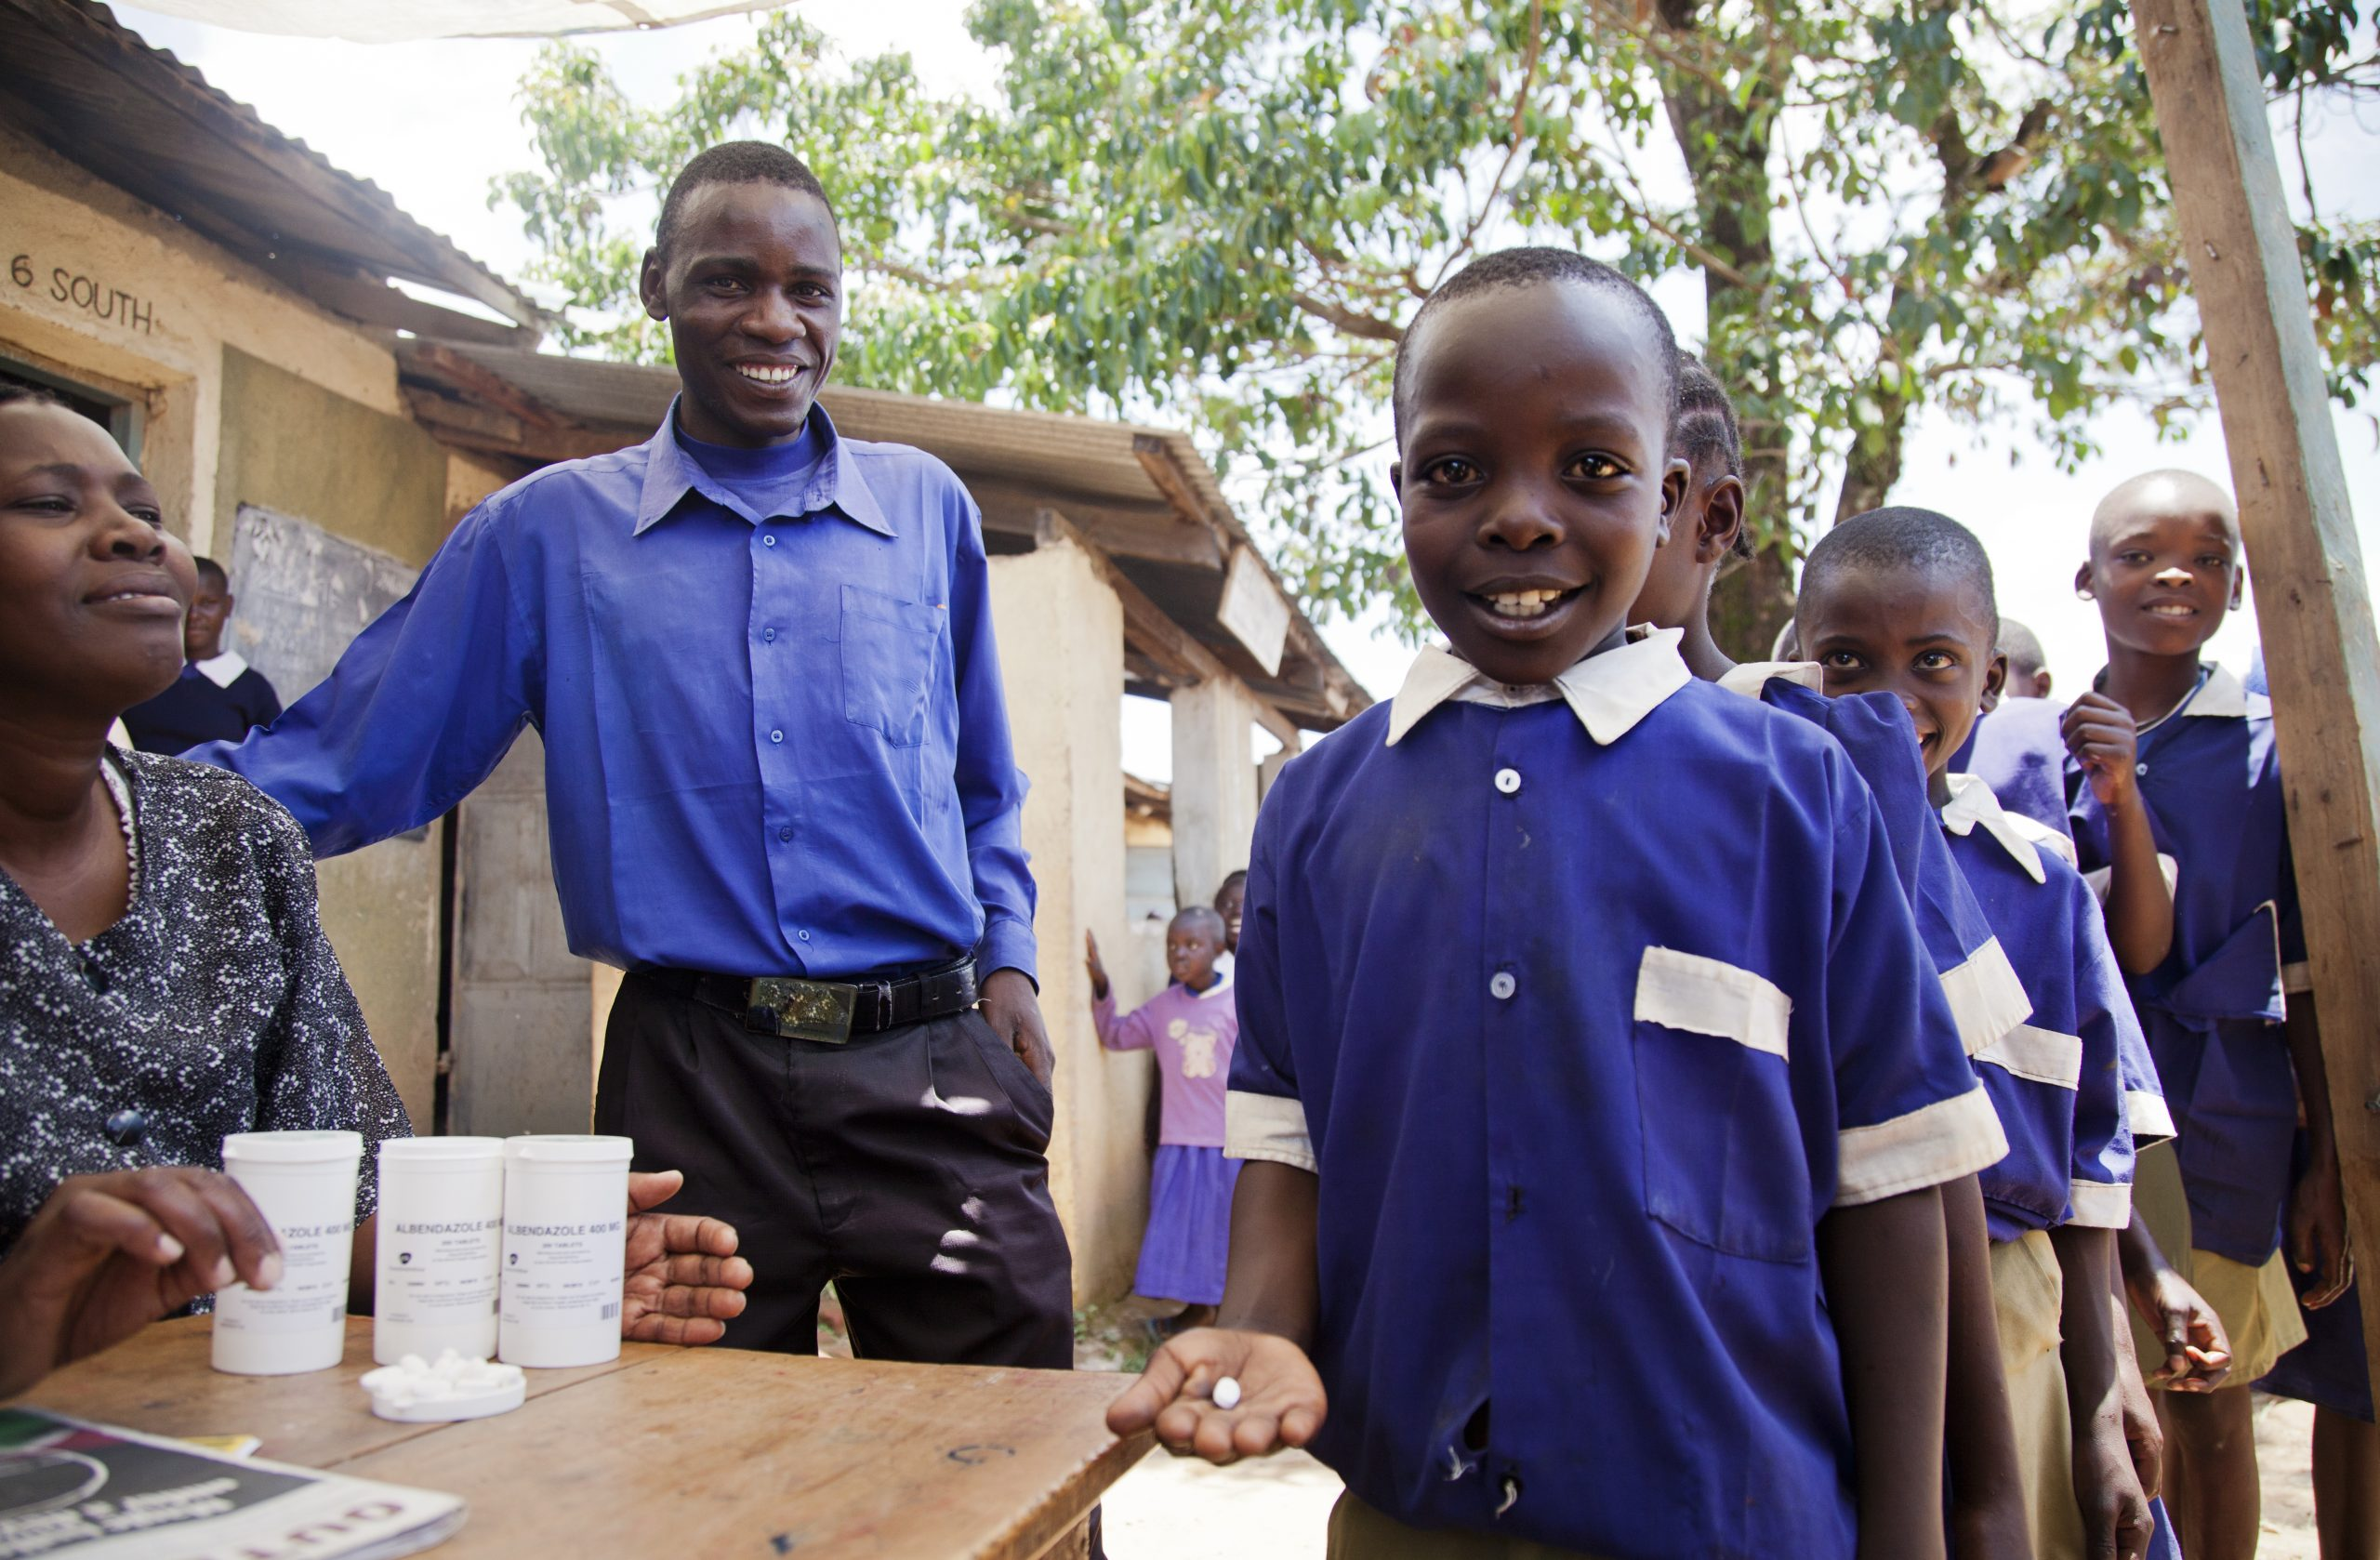
\includegraphics[keepaspectratio,height=3.6cm]{photos/Kenya-Deworm-the-World-Stephanie-Skinner.jpg}};
	
	\pgfmathsetmacro\xshift{0.5cm};
	\pgfmathsetmacro\yshift{5.75cm};
	%	\pgfmathsetmacro\mycolor{"gray"};
	
	\node[anchor=north west,align=left,text width = 9.5cm,xshift=\xshift,yshift=\yshift] (text1) at (0,0) {\textbf{Null hypothesis ($H_0$):}};
	\node[anchor=north west,align=left,text width = 9.5cm] (text2) at (text1.south west) {The average treatment effect is zero:  $ATE=0$};	
	\node[anchor=north west,align=left,text width = 9.5cm] (text3) at (text2.south west) {Or, equivalently:  $\bar{Y}_T = \bar{Y}_C$};	
	
	\node [anchor=north west,xshift=\xshift,yshift=\yshift] (fig) at (0,-1.9) {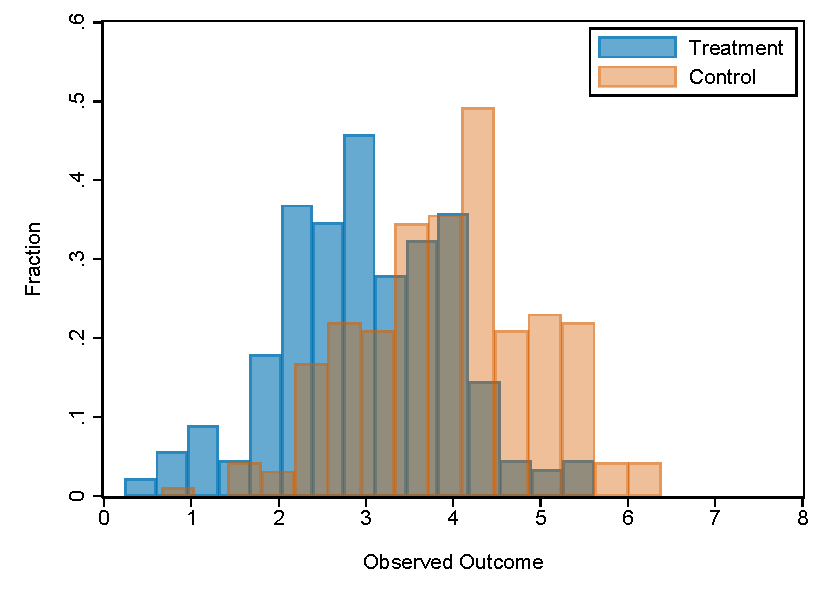
\includegraphics[keepaspectratio,height=3.6cm]{fig/TvsC-hist.pdf}};
	%\node [oiverm,anchor=west, text width = 4cm] (fig) at (fig.east) {In Stata: \\
		%\texttt{ttest y, by(t)}};
	
	\end{tikzpicture}
\end{center}

\end{frame}



%%%%%%%%%%%%%%%%%%%%%%%%%%%%%%%%%%%%%%%%%%%%%%%%%%%%%%%%%%%%%%%%%%%%%

\begin{frame}{$H_0$:  $ATE = 0$}

\begin{center}
	\begin{tikzpicture}
	
	% blank canvas
	\only<handout>{\fill[fill=white,draw=white,ultra thin]
		(0,0) -- (11,0) -- (11,6) -- (0,6) -- cycle;}
	\only<beamer>{\fill[fill=white,draw=white,ultra thin]
		(0,0) -- (14,0) -- (14,6) -- (0,6) -- cycle;}
	\only<beamer>{\draw[draw=oiblue!60,fill=oiblue!10,opacity=0.5] (11,1) rectangle (14,5);}
	%\draw[step=1.0,gray!20,thin] (0,0) grid (11,6);
	
	%\node [anchor=north] (photo) at (5,5.875) {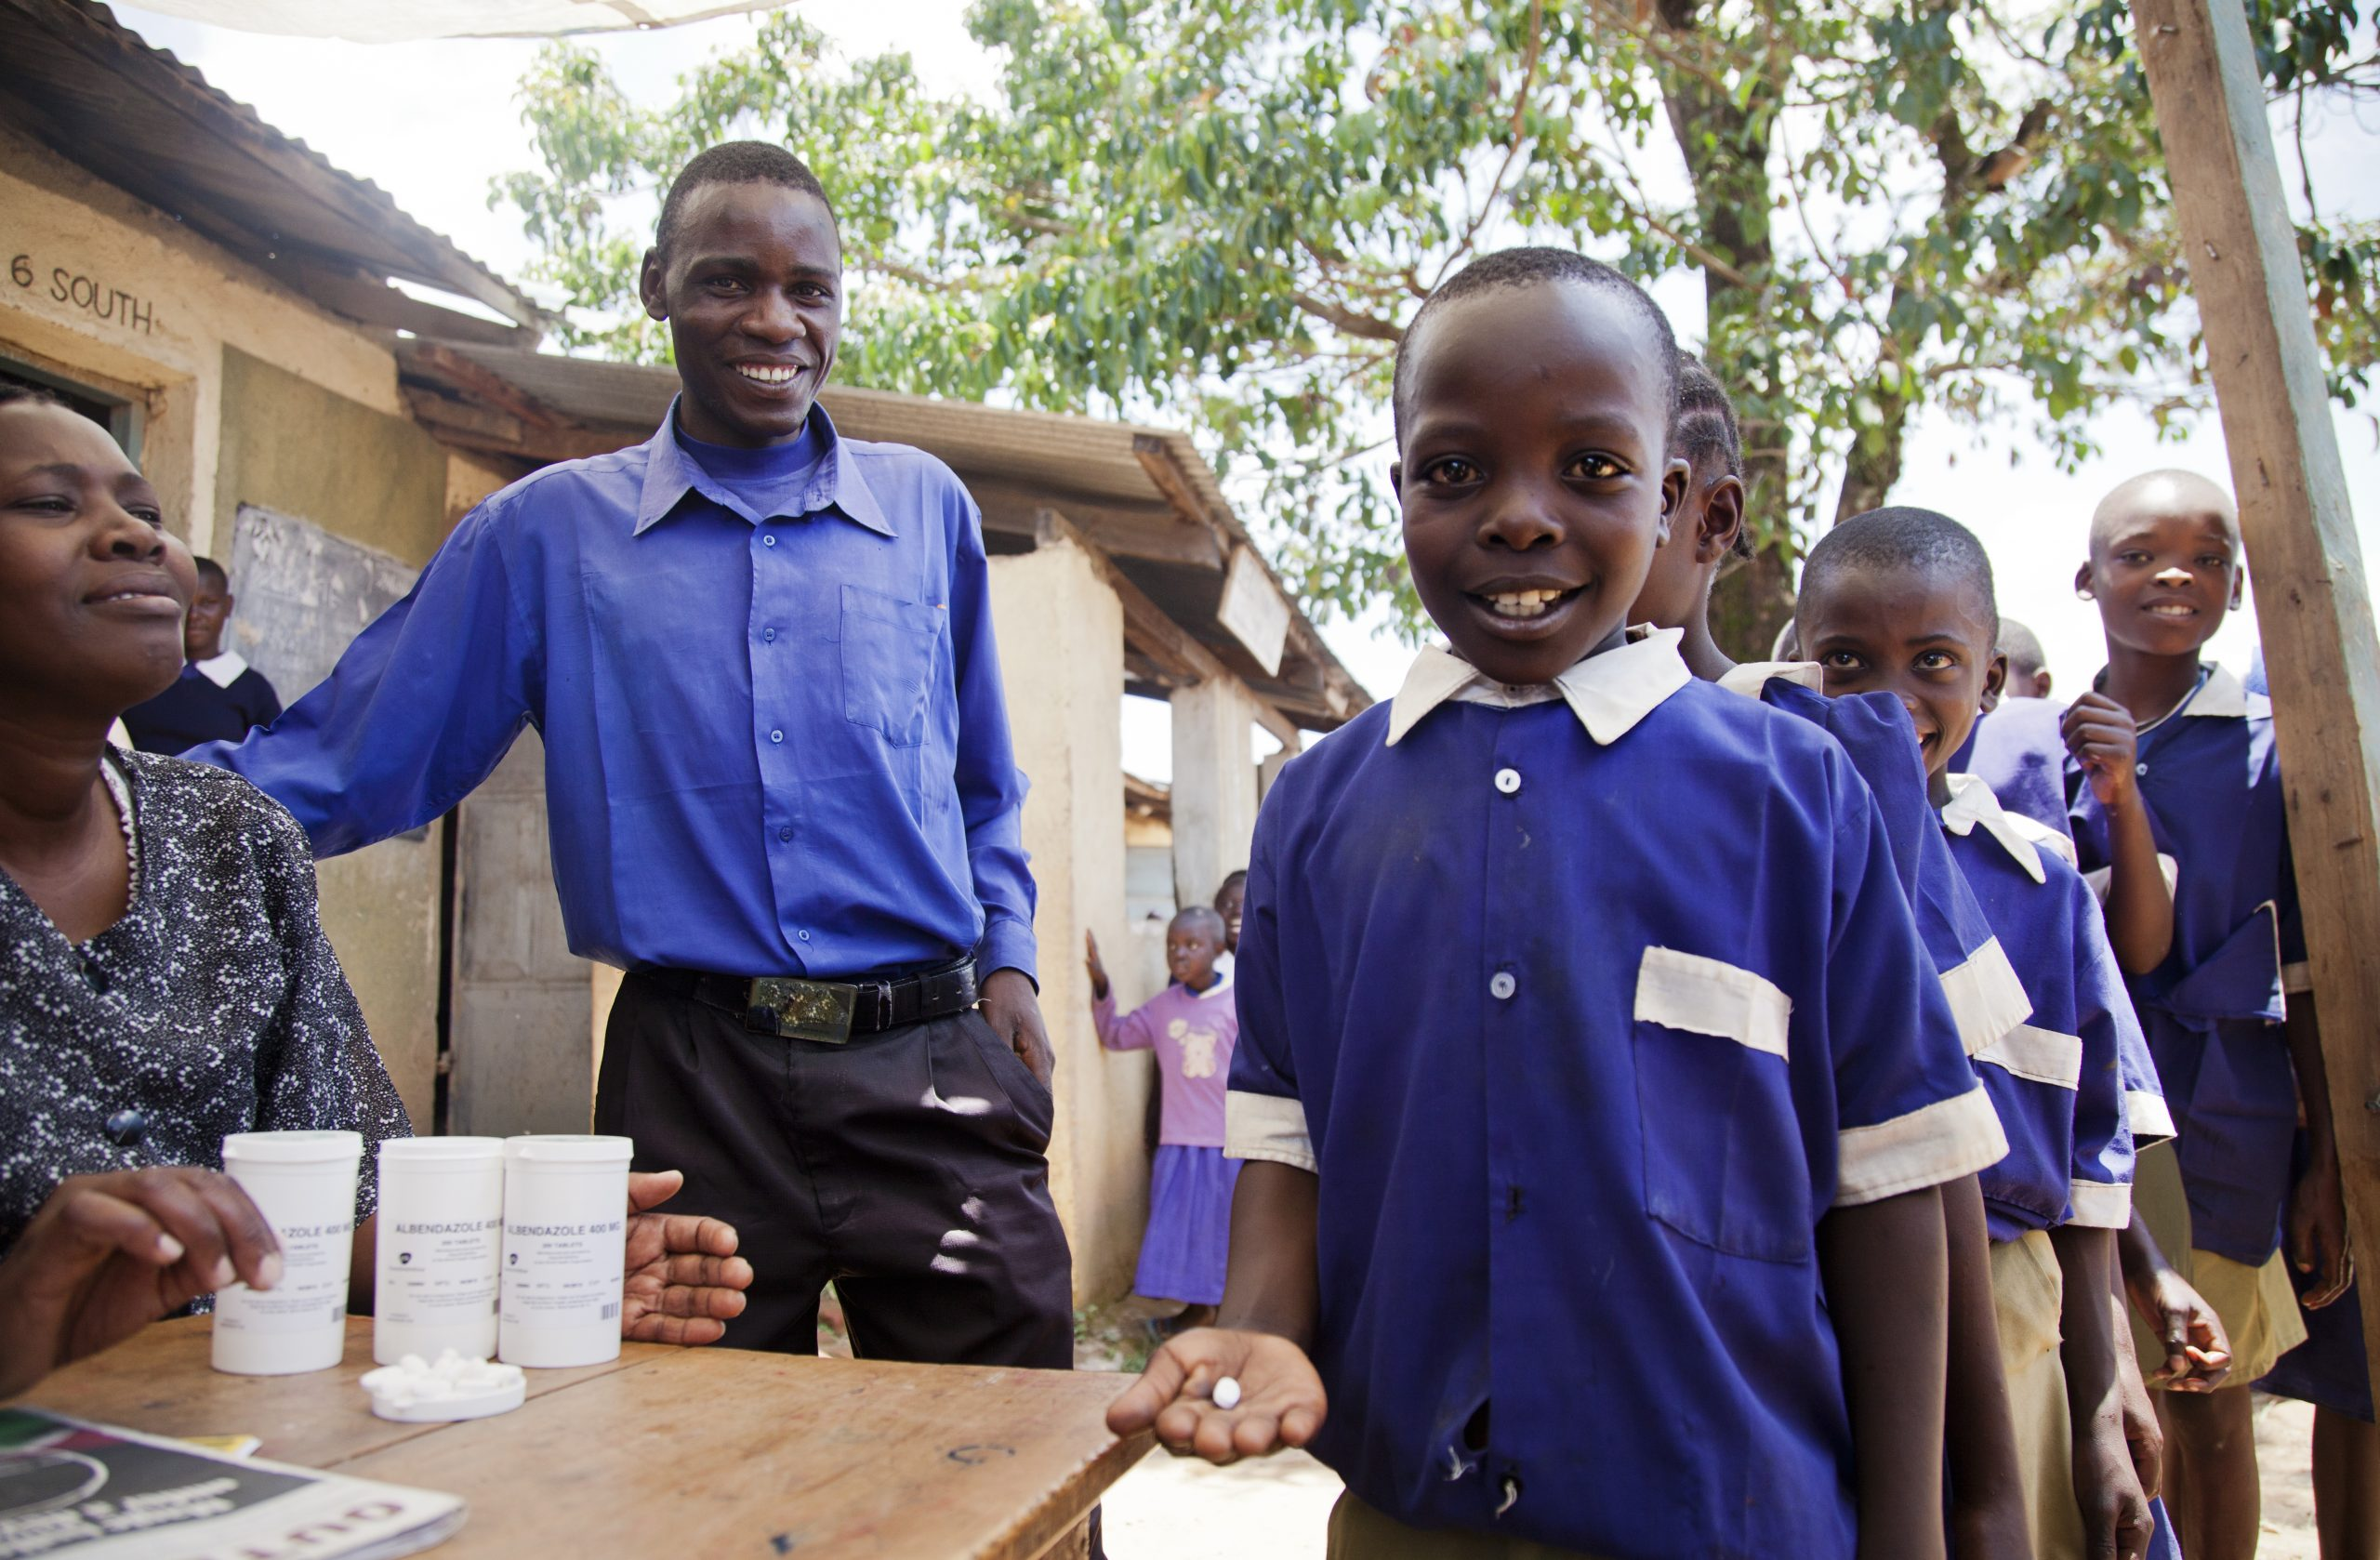
\includegraphics[keepaspectratio,height=3.6cm]{photos/Kenya-Deworm-the-World-Stephanie-Skinner.jpg}};
	
	\pgfmathsetmacro\xshift{0.5cm};
	\pgfmathsetmacro\yshift{5.75cm};
	%	\pgfmathsetmacro\mycolor{"gray"};
	
	\node[anchor=north west,align=left,text width = 9.5cm,xshift=\xshift,yshift=\yshift] (text1) at (0,0) {\textbf{Null hypothesis ($H_0$):}};
	\node[anchor=north west,align=left,text width = 9.5cm] (text2) at (text1.south west) {The average treatment effect is zero:  $ATE=0$};	
	\node[anchor=north west,align=left,text width = 9.5cm] (text3) at (text2.south west) {Or, equivalently:  $\bar{Y}_T = \bar{Y}_C$};	
	
	\node [anchor=north west,xshift=\xshift,yshift=\yshift] (fig) at (0,-1.9) {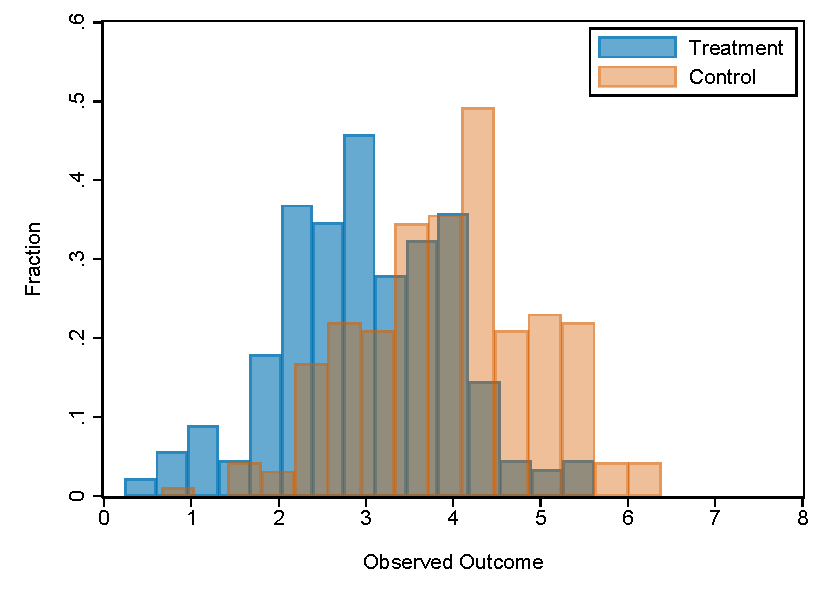
\includegraphics[keepaspectratio,height=3.6cm]{fig/TvsC-hist.pdf}};
	\node [oiblue,anchor=west, text width = 4cm] (fig) at (fig.east) {In Stata: \\
		\texttt{ttest y, by(t)}};
	
	\end{tikzpicture}
\end{center}

\end{frame}


%%%%%%%%%%%%%%%%%%%%%%%%%%%%%%%%%%%%%%%%%%%%%%%%%%%%%%%%%%%%%%%%%%%%%

\begin{frame}<handout:0>{Testing the Equality of Means}

\begin{center}
	\begin{tikzpicture}
	
	% blank canvas
	\only<handout>{\fill[fill=white,draw=white,ultra thin]
		(0,0) -- (11,0) -- (11,6) -- (0,6) -- cycle;}
	\only<beamer>{\fill[fill=white,draw=white,ultra thin]
		(0,0) -- (14,0) -- (14,6) -- (0,6) -- cycle;}
	\only<beamer>{\draw[draw=oiblue!60,fill=oiblue!10,opacity=0.5] (11,1) rectangle (14,5);}
	%\draw[step=1.0,gray!20,thin] (0,0) grid (11,6);
	
	%\node [anchor=north] (photo) at (5,5.875) {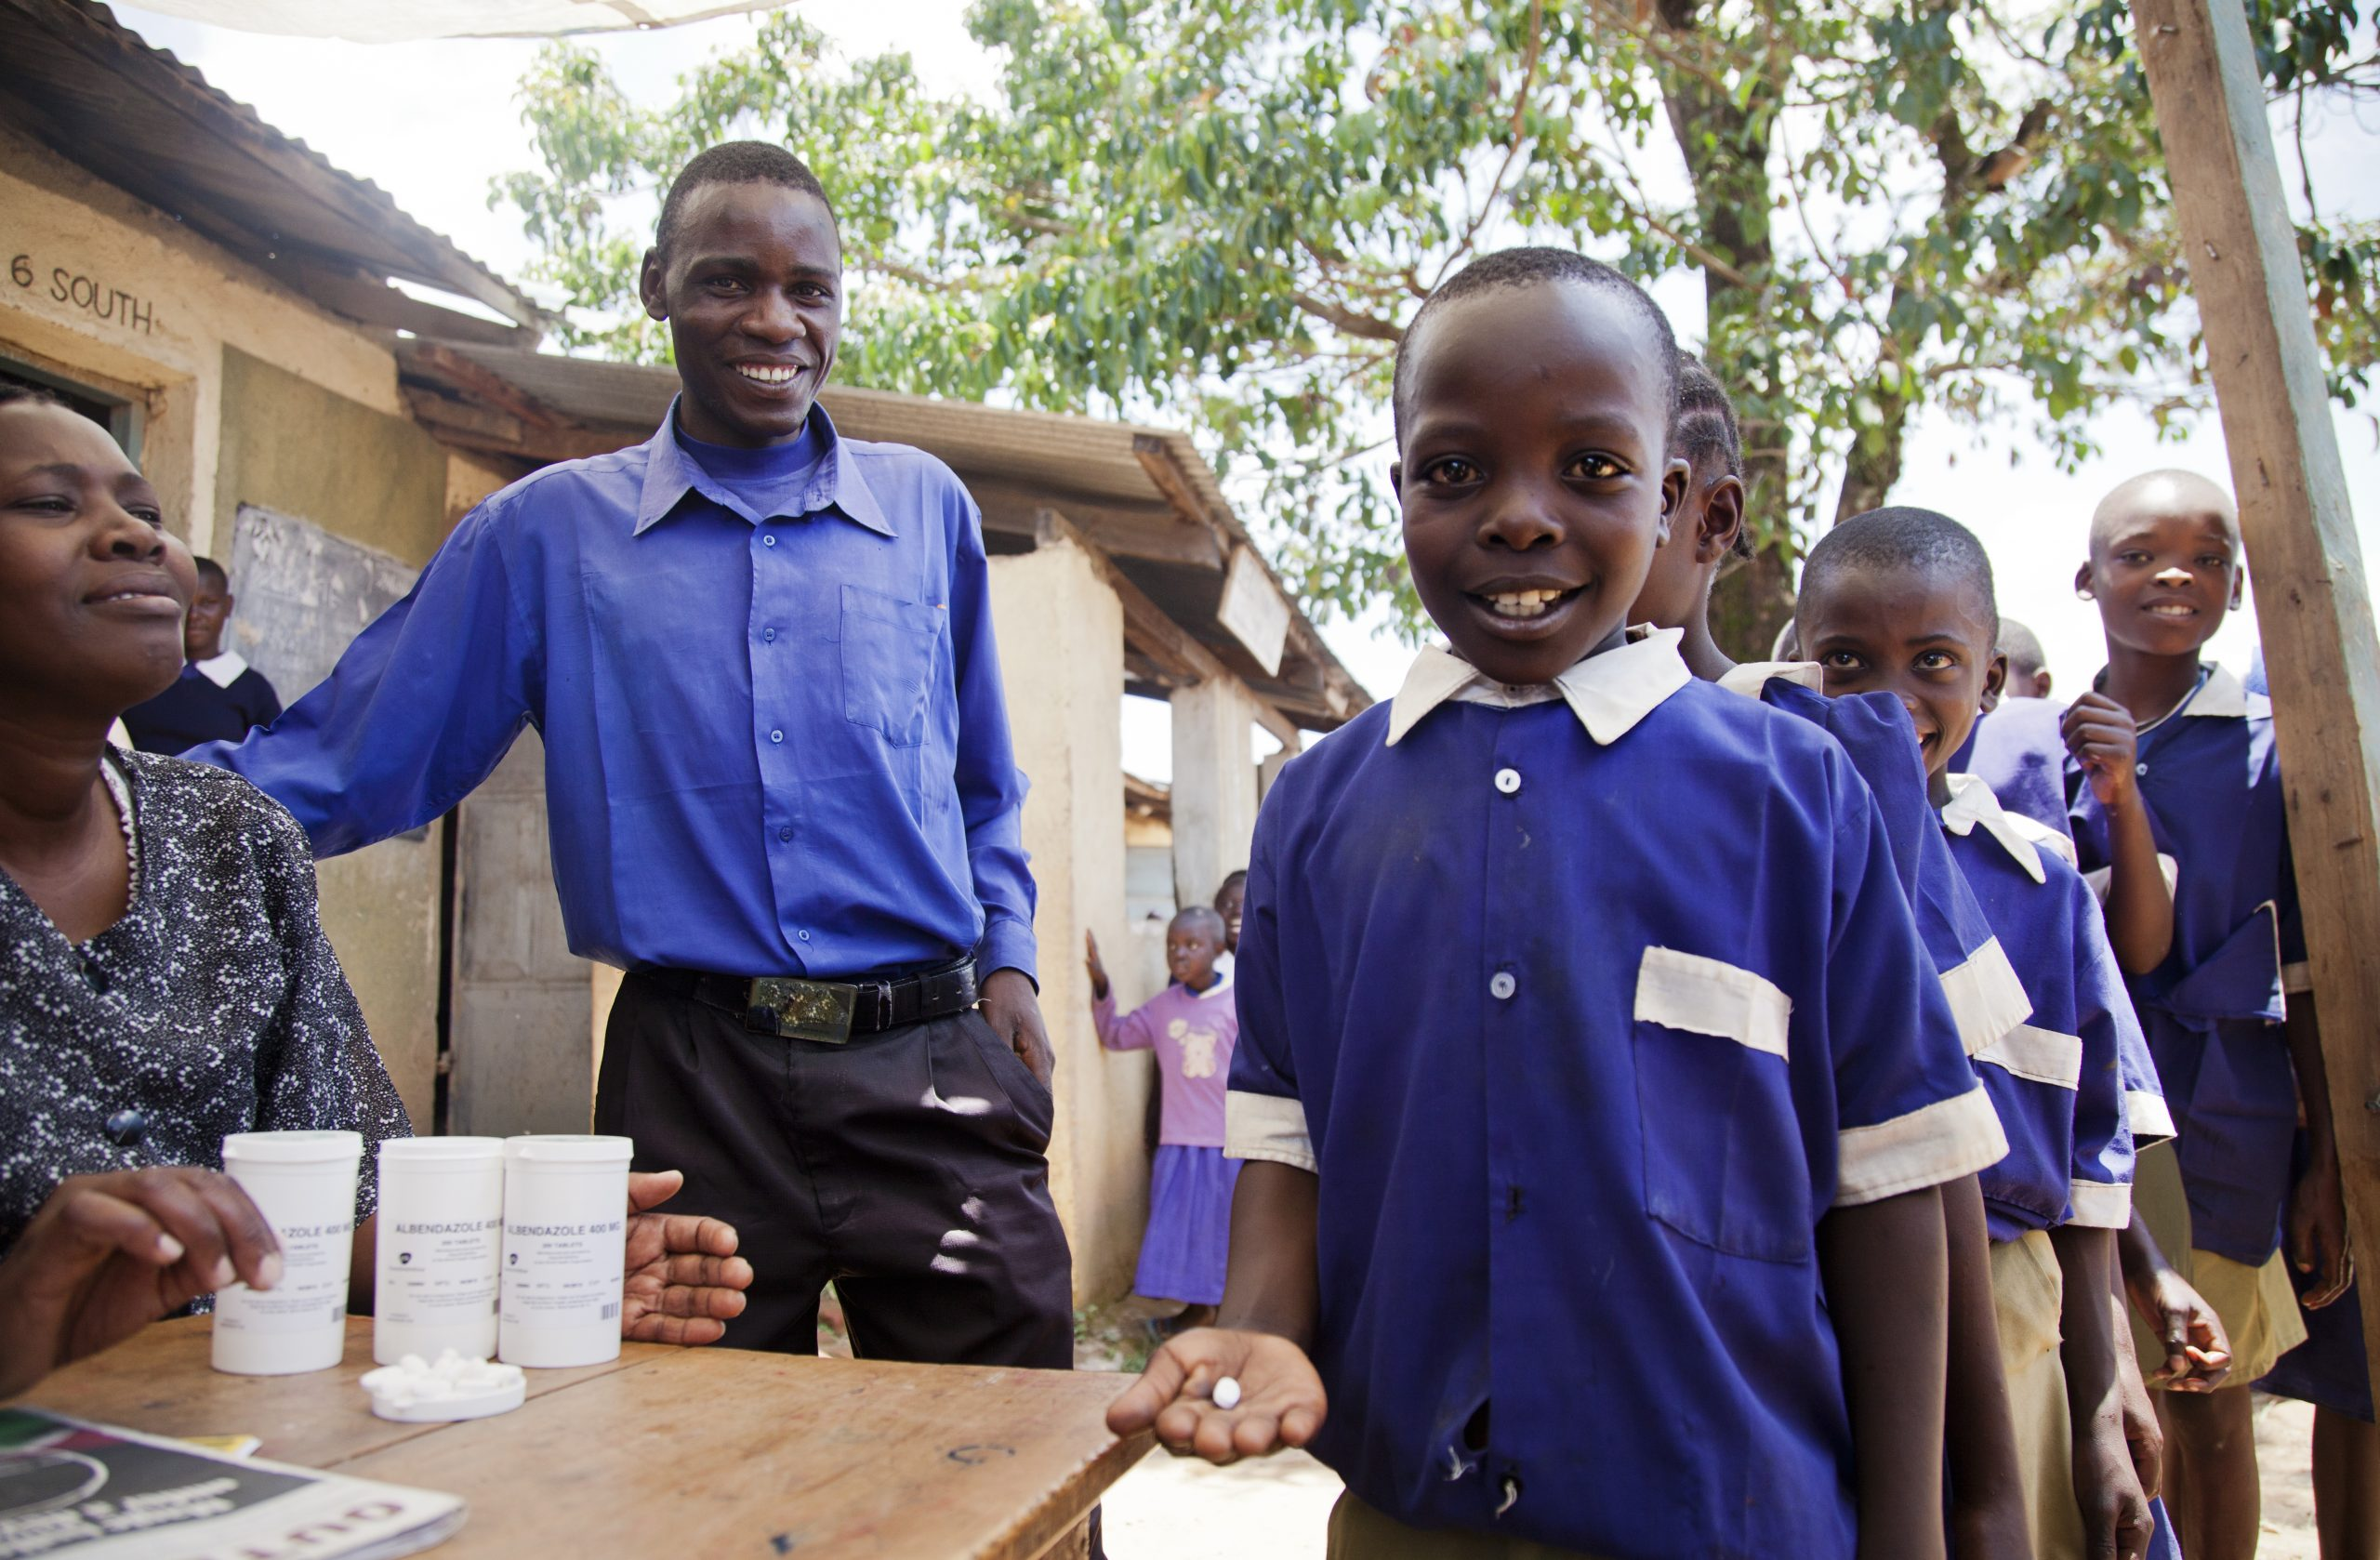
\includegraphics[keepaspectratio,height=3.6cm]{photos/Kenya-Deworm-the-World-Stephanie-Skinner.jpg}};
	
	\pgfmathsetmacro\xshift{0.5cm};
	\pgfmathsetmacro\yshift{5.75cm};
	%	\pgfmathsetmacro\mycolor{"gray"};
	
	\node[oiblue,anchor=north west,align=left,text width = 9.5cm,xshift=\xshift,yshift=\yshift] (text1) at (0,0) {Stata:  \texttt{ttest y, by(t)}};
	
	
	\node [anchor=north west,xshift=\xshift,yshift=\yshift] (fig) at (0,-1) {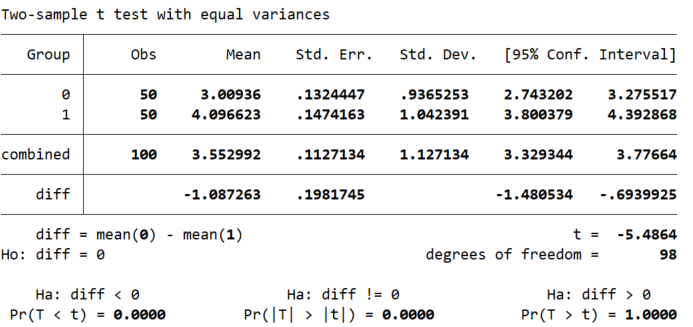
\includegraphics[keepaspectratio,width=8cm]{img/stata-ttest-output.png}};
	\node[red,anchor=west] (lbl1) at (6,5.5) {control group mean};
	\draw[red,->,thick] (lbl1.west) -- (3.7,3.55);
	%\node[red,anchor=west] (lbl2) at (6,4.75) {treatment group mean};
	%\draw[red,->,thick] (lbl2.west) -- (3.7,3.28);
	%\node[red,anchor=west] (lbl3) at (8.75,4) {difference};
	%\draw[red,->,thick] (lbl3.west) -- (3.7,2.4);
	%\node[red,anchor=west] (lbl4) at (9.5,2) {t-stat};
	%\draw[red,->,thick] (lbl4.west) -- (8.5,1.92);
	%\node[red,anchor=west] (lbl5) at (7,0.5) {p-value};
	%\draw[red,->,thick] (lbl5.west) -- (5.72,1);
	
	\end{tikzpicture}
\end{center}

\end{frame}


%%%%%%%%%%%%%%%%%%%%%%%%%%%%%%%%%%%%%%%%%%%%%%%%%%%%%%%%%%%%%%%%%%%%%

\begin{frame}<handout:0>{Testing the Equality of Means}

\begin{center}
	\begin{tikzpicture}
	
	% blank canvas
	\only<handout>{\fill[fill=white,draw=white,ultra thin]
		(0,0) -- (11,0) -- (11,6) -- (0,6) -- cycle;}
	\only<beamer>{\fill[fill=white,draw=white,ultra thin]
		(0,0) -- (14,0) -- (14,6) -- (0,6) -- cycle;}
	\only<beamer>{\draw[draw=oiblue!60,fill=oiblue!10,opacity=0.5] (11,1) rectangle (14,5);}
	%\draw[step=1.0,gray!20,thin] (0,0) grid (11,6);
	
	%\node [anchor=north] (photo) at (5,5.875) {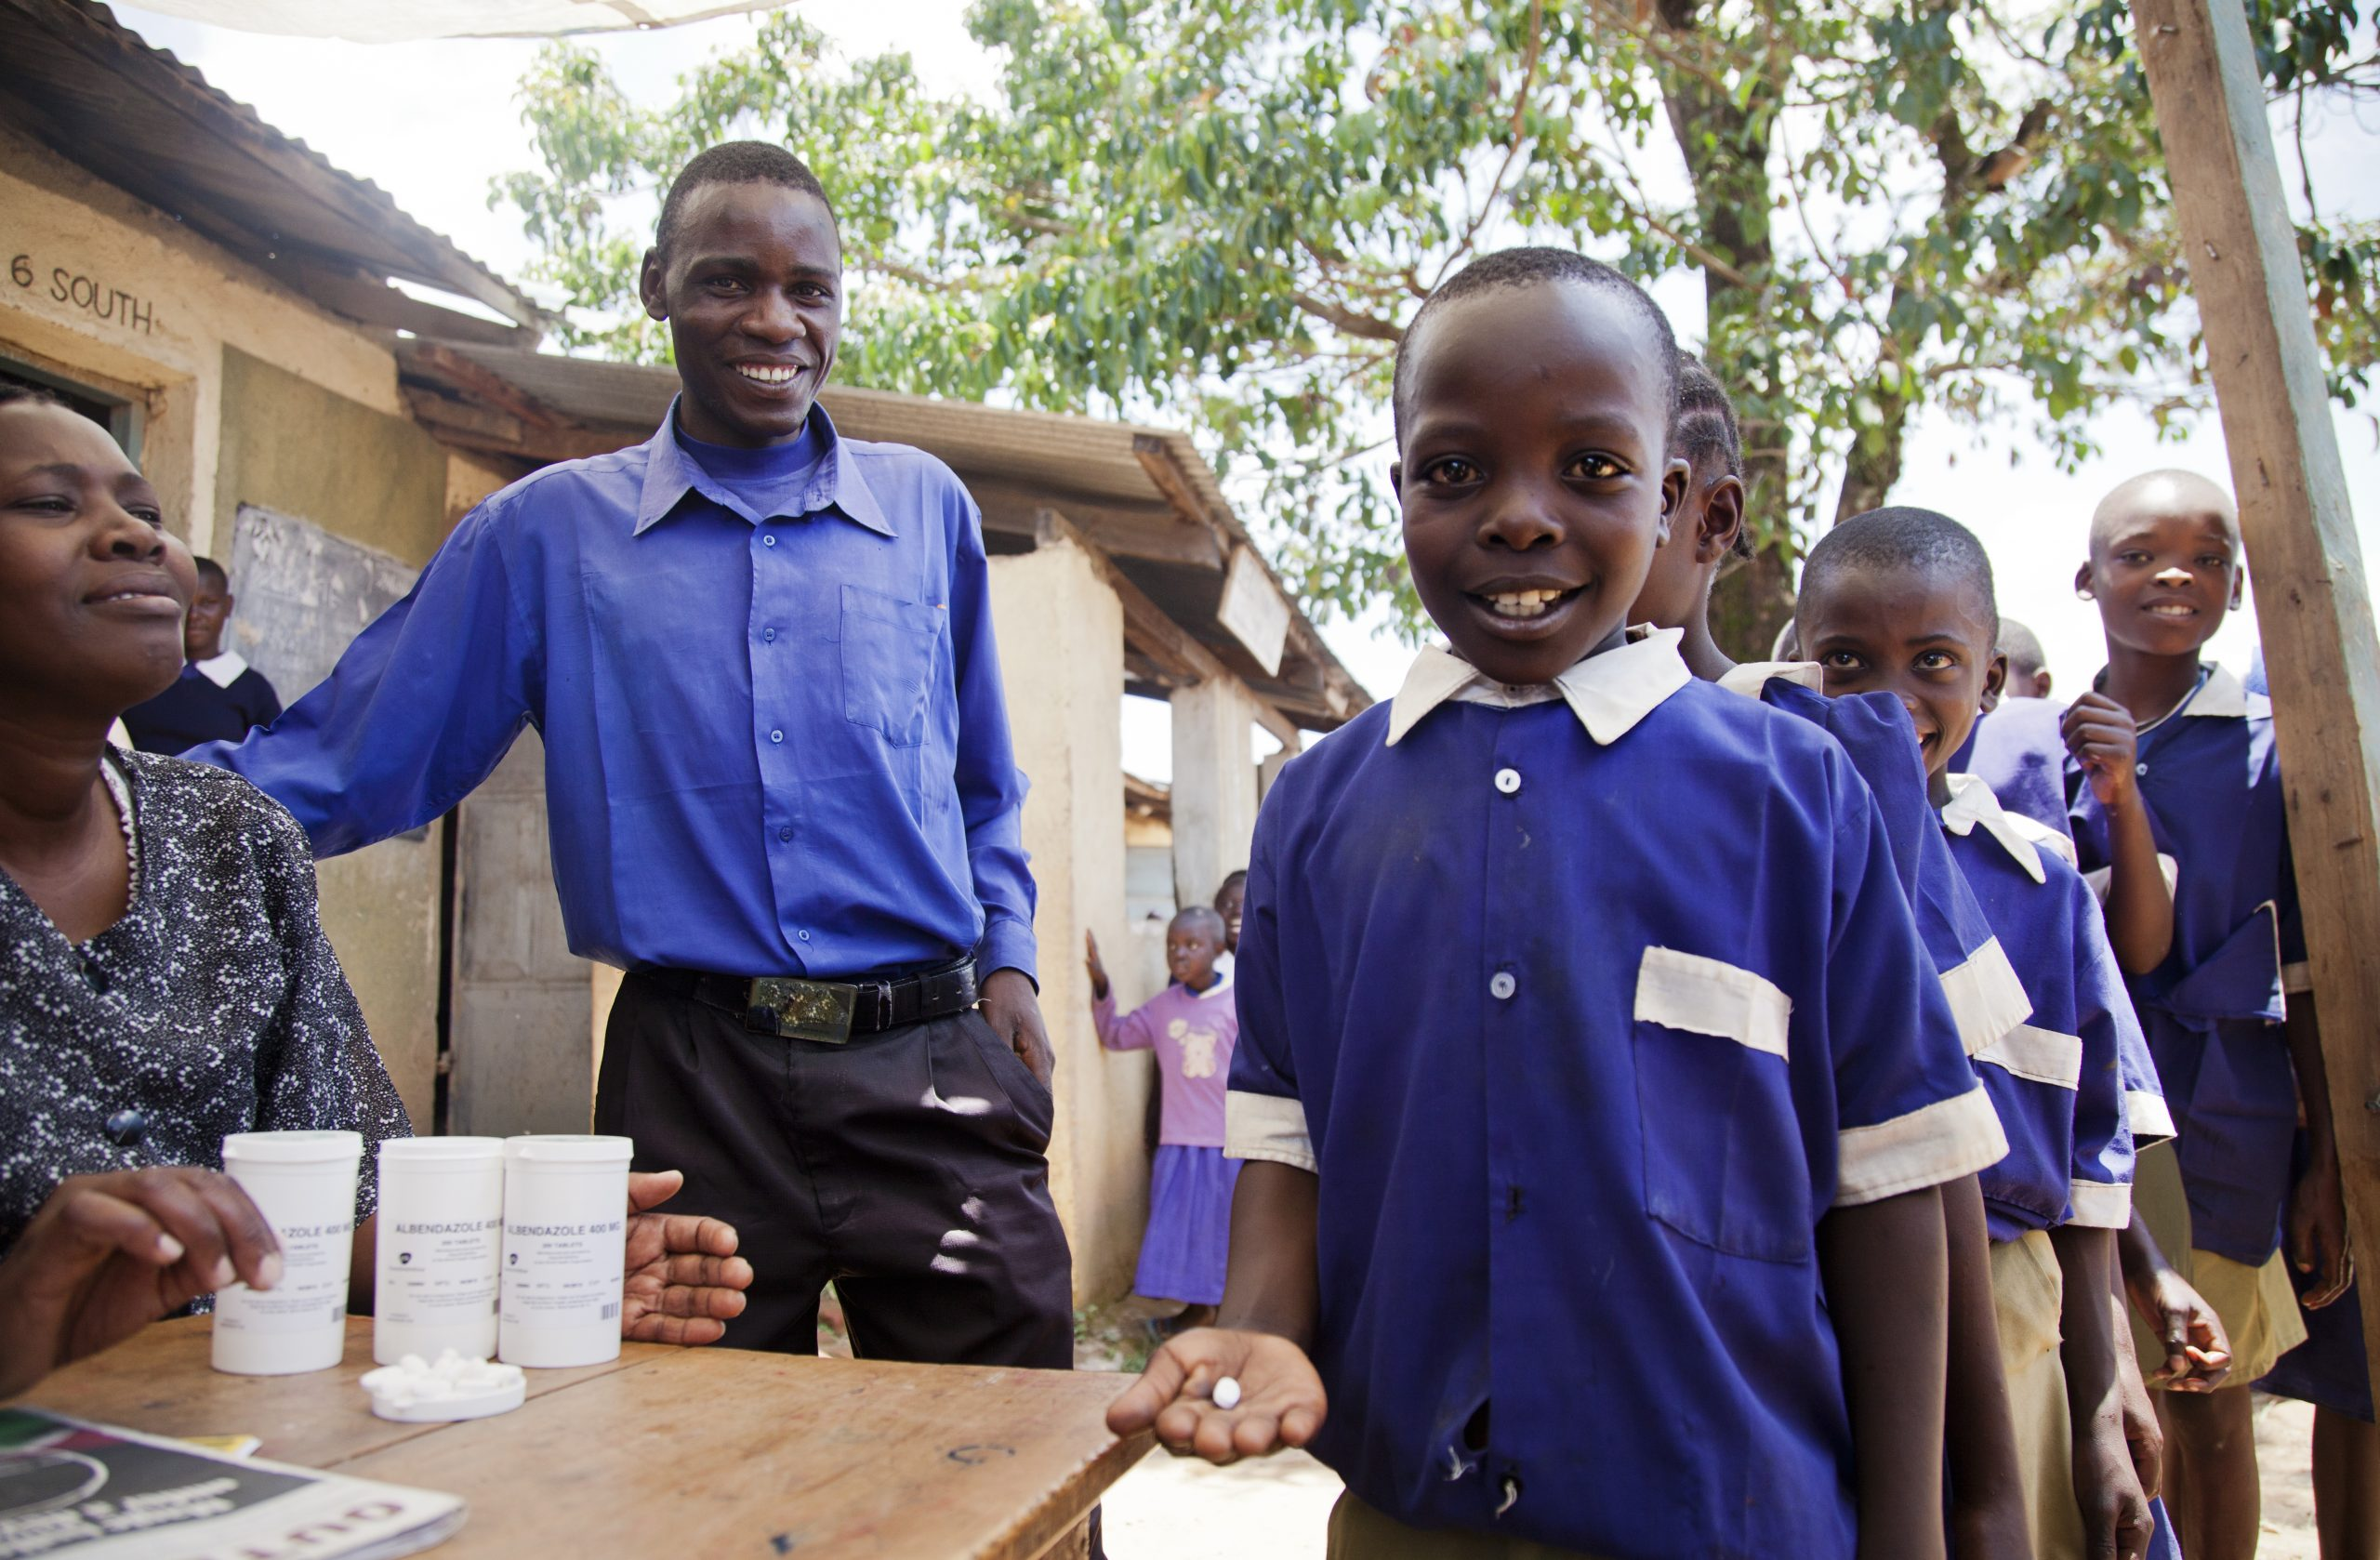
\includegraphics[keepaspectratio,height=3.6cm]{photos/Kenya-Deworm-the-World-Stephanie-Skinner.jpg}};
	
	\pgfmathsetmacro\xshift{0.5cm};
	\pgfmathsetmacro\yshift{5.75cm};
	%	\pgfmathsetmacro\mycolor{"gray"};
	
	\node[oiblue,anchor=north west,align=left,text width = 9.5cm,xshift=\xshift,yshift=\yshift] (text1) at (0,0) {Stata:  \texttt{ttest y, by(t)}};
	
	
	\node [anchor=north west,xshift=\xshift,yshift=\yshift] (fig) at (0,-1) {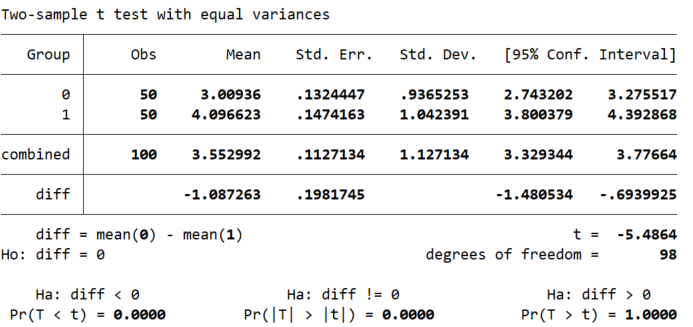
\includegraphics[keepaspectratio,width=8cm]{img/stata-ttest-output.png}};
	\node[gray,anchor=west] (lbl1) at (6,5.5) {control group mean};
	\draw[gray,->,thick] (lbl1.west) -- (3.7,3.55);
	\node[red,anchor=west] (lbl2) at (6,4.75) {treatment group mean};
	\draw[red,->,thick] (lbl2.west) -- (3.7,3.28);
	%\node[red,anchor=west] (lbl3) at (8.75,4) {difference};
	%\draw[red,->,thick] (lbl3.west) -- (3.7,2.4);
	%\node[red,anchor=west] (lbl4) at (9.5,2) {t-stat};
	%\draw[red,->,thick] (lbl4.west) -- (8.5,1.92);
	%\node[red,anchor=west] (lbl5) at (7,0.5) {p-value};
	%\draw[red,->,thick] (lbl5.west) -- (5.72,1);
	
	\end{tikzpicture}
\end{center}

\end{frame}


%%%%%%%%%%%%%%%%%%%%%%%%%%%%%%%%%%%%%%%%%%%%%%%%%%%%%%%%%%%%%%%%%%%%%

\begin{frame}<handout:0>{Testing the Equality of Means}

\begin{center}
	\begin{tikzpicture}
	
	% blank canvas
	\only<handout>{\fill[fill=white,draw=white,ultra thin]
		(0,0) -- (11,0) -- (11,6) -- (0,6) -- cycle;}
	\only<beamer>{\fill[fill=white,draw=white,ultra thin]
		(0,0) -- (14,0) -- (14,6) -- (0,6) -- cycle;}
	\only<beamer>{\draw[draw=oiblue!60,fill=oiblue!10,opacity=0.5] (11,1) rectangle (14,5);}
	%\draw[step=1.0,gray!20,thin] (0,0) grid (11,6);
	
	%\node [anchor=north] (photo) at (5,5.875) {\includegraphics[keepaspectratio,height=3.6cm]{photos/Kenya-Deworm-the-World-Stephanie-Skinner.jpg}};
	
	\pgfmathsetmacro\xshift{0.5cm};
	\pgfmathsetmacro\yshift{5.75cm};
	%	\pgfmathsetmacro\mycolor{"gray"};
	
	\node[oiblue,anchor=north west,align=left,text width = 9.5cm,xshift=\xshift,yshift=\yshift] (text1) at (0,0) {Stata:  \texttt{ttest y, by(t)}};
	
	
	\node [anchor=north west,xshift=\xshift,yshift=\yshift] (fig) at (0,-1) {\includegraphics[keepaspectratio,width=8cm]{img/stata-ttest-output.png}};
	\node[gray,anchor=west] (lbl1) at (6,5.5) {control group mean};
	\draw[gray,->,thick] (lbl1.west) -- (3.7,3.55);
	\node[gray,anchor=west] (lbl2) at (6,4.75) {treatment group mean};
	\draw[gray,->,thick] (lbl2.west) -- (3.7,3.28);
	\node[red,anchor=west] (lbl3) at (8.75,4) {difference};
	\draw[red,->,thick] (lbl3.west) -- (3.7,2.4);
	%\node[red,anchor=west] (lbl4) at (9.5,2) {t-stat};
	%\draw[red,->,thick] (lbl4.west) -- (8.5,1.92);
	%\node[red,anchor=west] (lbl5) at (7,0.5) {p-value};
	%\draw[red,->,thick] (lbl5.west) -- (5.72,1);
	
	\end{tikzpicture}
\end{center}

\end{frame}



%%%%%%%%%%%%%%%%%%%%%%%%%%%%%%%%%%%%%%%%%%%%%%%%%%%%%%%%%%%%%%%%%%%%%

\begin{frame}<handout:0>{Testing the Equality of Means}

\begin{center}
	\begin{tikzpicture}
	
	% blank canvas
	\only<handout>{\fill[fill=white,draw=white,ultra thin]
		(0,0) -- (11,0) -- (11,6) -- (0,6) -- cycle;}
	\only<beamer>{\fill[fill=white,draw=white,ultra thin]
		(0,0) -- (14,0) -- (14,6) -- (0,6) -- cycle;}
	\only<beamer>{\draw[draw=oiblue!60,fill=oiblue!10,opacity=0.5] (11,1) rectangle (14,5);}
	%\draw[step=1.0,gray!20,thin] (0,0) grid (11,6);
	
	%\node [anchor=north] (photo) at (5,5.875) {\includegraphics[keepaspectratio,height=3.6cm]{photos/Kenya-Deworm-the-World-Stephanie-Skinner.jpg}};
	
	\pgfmathsetmacro\xshift{0.5cm};
	\pgfmathsetmacro\yshift{5.75cm};
	%	\pgfmathsetmacro\mycolor{"gray"};
	
	\node[oiblue,anchor=north west,align=left,text width = 9.5cm,xshift=\xshift,yshift=\yshift] (text1) at (0,0) {Stata:  \texttt{ttest y, by(t)}};
	
	
	\node [anchor=north west,xshift=\xshift,yshift=\yshift] (fig) at (0,-1) {\includegraphics[keepaspectratio,width=8cm]{img/stata-ttest-output.png}};
	\node[gray,anchor=west] (lbl1) at (6,5.5) {control group mean};
	\draw[gray,->,thick] (lbl1.west) -- (3.7,3.55);
	\node[gray,anchor=west] (lbl2) at (6,4.75) {treatment group mean};
	\draw[gray,->,thick] (lbl2.west) -- (3.7,3.28);
	\node[gray,anchor=west] (lbl3) at (8.75,4) {difference};
	\draw[gray,->,thick] (lbl3.west) -- (3.7,2.4);
	\node[red,anchor=west] (lbl4) at (9.5,2) {t-stat};
	\draw[red,->,thick] (lbl4.west) -- (8.5,1.92);
	%\node[red,anchor=west] (lbl5) at (7,0.5) {p-value};
	%\draw[red,->,thick] (lbl5.west) -- (5.72,1);
	
	\end{tikzpicture}
\end{center}

\end{frame}


%%%%%%%%%%%%%%%%%%%%%%%%%%%%%%%%%%%%%%%%%%%%%%%%%%%%%%%%%%%%%%%%%%%%%

\begin{frame}{Testing the Equality of Means}

\begin{center}
	\begin{tikzpicture}
	
	% blank canvas
	\only<handout>{\fill[fill=white,draw=white,ultra thin]
		(0,0) -- (11,0) -- (11,6) -- (0,6) -- cycle;}
	\only<beamer>{\fill[fill=white,draw=white,ultra thin]
		(0,0) -- (14,0) -- (14,6) -- (0,6) -- cycle;}
	\only<beamer>{\draw[draw=oiblue!60,fill=oiblue!10,opacity=0.5] (11,1) rectangle (14,5);}
	%\draw[step=1.0,gray!20,thin] (0,0) grid (11,6);
	
	%\node [anchor=north] (photo) at (5,5.875) {\includegraphics[keepaspectratio,height=3.6cm]{photos/Kenya-Deworm-the-World-Stephanie-Skinner.jpg}};
	
	\pgfmathsetmacro\xshift{0.5cm};
	\pgfmathsetmacro\yshift{5.75cm};
	%	\pgfmathsetmacro\mycolor{"gray"};
	
	\node[oiblue,anchor=north west,align=left,text width = 9.5cm,xshift=\xshift,yshift=\yshift] (text1) at (0,0) {Stata:  \texttt{ttest y, by(t)}};
	
	
	\node [anchor=north west,xshift=\xshift,yshift=\yshift] (fig) at (0,-1) {\includegraphics[keepaspectratio,width=8cm]{img/stata-ttest-output.png}};
	\node[gray,anchor=west] (lbl1) at (6,5.5) {control group mean};
	\draw[gray,->,thick] (lbl1.west) -- (3.7,3.55);
	\node[gray,anchor=west] (lbl2) at (6,4.75) {treatment group mean};
	\draw[gray,->,thick] (lbl2.west) -- (3.7,3.28);
	\node[gray,anchor=west] (lbl3) at (8.75,4) {difference};
	\draw[gray,->,thick] (lbl3.west) -- (3.7,2.4);
	\node[gray,anchor=west] (lbl4) at (9.5,2) {t-stat};
	\draw[gray,->,thick] (lbl4.west) -- (8.5,1.92);
	\node[red,anchor=west] (lbl5) at (7,0.5) {p-value};
	\draw[red,->,thick] (lbl5.west) -- (5.72,1);
	
	\end{tikzpicture}
\end{center}

\end{frame}


%%%%%%%%%%%%%%%%%%%%%%%%%%%%%%%%%%%%%%%%%%%%%%%%%%%%%%%%%%%%%%%%%%%%%

\begin{frame}{Regression Analysis of RCTs}

\medskip
\begin{center}
	\includegraphics[width=0.72\textwidth]{fig/reg-w-continuous-x.pdf}
\end{center}

%Simple regression framework for analyzing RCTs: \structure{$Y_i = \alpha + \beta D_i + \varepsilon_i$}
%
%\medskip
%\begin{itemize}
%	
%	\item Treatment indicator $D_i = 0,1$ $\Rightarrow$ only two possible values of $\hat{Y_i}$
%	
%\end{itemize}

\end{frame}




%%%%%%%%%%%%%%%%%%%%%%%%%%%%%%%%%%%%%%%%%%%%%%%%%%%%%%%%%%%%%%%%%%%%%

\begin{frame}{Regression Analysis of RCTs}

\medskip
\begin{center}
	\includegraphics[width=0.54\textwidth]{fig/TvsCreg.pdf}
\end{center}

Simple regression framework for analyzing RCTs: \textcolor{red}{$Y_i = \alpha + \beta D_i + \varepsilon_i$}

\medskip
\begin{itemize}
	
	\item Treatment indicator $D_i = 0,1$ $\Rightarrow$ only two possible values of $\hat{Y_i}$
	
\end{itemize}

\end{frame}


%%%%%%%%%%%%%%%%%%%%%%%%%%%%%%%%%%%%%%%%%%%%%%%%%%%%%%%%%%%%%%%%%%%%%

\begin{frame}<handout:0>{Regression Analysis of RCTs}

\begin{center}
	\begin{tikzpicture}
	
	% blank canvas
	\only<handout>{\fill[fill=white,draw=white,ultra thin]
		(0,0) -- (11,0) -- (11,6) -- (0,6) -- cycle;}
	\only<beamer>{\fill[fill=white,draw=white,ultra thin]
		(0,0) -- (14,0) -- (14,6) -- (0,6) -- cycle;}
	\only<beamer>{\draw[draw=oiblue!60,fill=oiblue!10,opacity=0.5] (11,1) rectangle (14,5);}
	%\draw[step=1.0,gray!20,thin] (0,0) grid (11,6);
	
	%\node [anchor=north] (photo) at (5,5.875) {\includegraphics[keepaspectratio,height=3.6cm]{photos/Kenya-Deworm-the-World-Stephanie-Skinner.jpg}};
	
	\pgfmathsetmacro\xshift{0.5cm};
	\pgfmathsetmacro\yshift{5.75cm};
	%	\pgfmathsetmacro\mycolor{"gray"};
	
	\node[oiblue,anchor=north west,align=left,text width = 9.5cm,xshift=\xshift,yshift=\yshift] (text1) at (0,0) {Stata:  \texttt{reg y t}};
	
	
	\node [anchor=north west,xshift=\xshift,yshift=\yshift] (fig) at (0,-1) {\includegraphics[keepaspectratio,width=8cm]{img/stata-reg-output.png}};
	\node[red,anchor=north,] (lbl1) at (2.75,1) {control group mean};
	\draw[red,->,thick] (lbl1.north) -- ([yshift=0.75cm]lbl1.north);
	
	\end{tikzpicture}
\end{center}

\end{frame}


%%%%%%%%%%%%%%%%%%%%%%%%%%%%%%%%%%%%%%%%%%%%%%%%%%%%%%%%%%%%%%%%%%%%%

\begin{frame}<handout:0>{Regression Analysis of RCTs}

\begin{center}
	\begin{tikzpicture}
	
	% blank canvas
	\only<handout>{\fill[fill=white,draw=white,ultra thin]
		(0,0) -- (11,0) -- (11,6) -- (0,6) -- cycle;}
	\only<beamer>{\fill[fill=white,draw=white,ultra thin]
		(0,0) -- (14,0) -- (14,6) -- (0,6) -- cycle;}
	\only<beamer>{\draw[draw=oiblue!60,fill=oiblue!10,opacity=0.5] (11,1) rectangle (14,5);}
	%\draw[step=1.0,gray!20,thin] (0,0) grid (11,6);
	
	%\node [anchor=north] (photo) at (5,5.875) {\includegraphics[keepaspectratio,height=3.6cm]{photos/Kenya-Deworm-the-World-Stephanie-Skinner.jpg}};
	
	\pgfmathsetmacro\xshift{0.5cm};
	\pgfmathsetmacro\yshift{5.75cm};
	%	\pgfmathsetmacro\mycolor{"gray"};
	
	\node[oiblue,anchor=north west,align=left,text width = 9.5cm,xshift=\xshift,yshift=\yshift] (text1) at (0,0) {Stata:  \texttt{reg y t}};
	
	
	\node [anchor=north west,xshift=\xshift,yshift=\yshift] (fig) at (0,-1) {\includegraphics[keepaspectratio,width=8cm]{img/stata-reg-output.png}};
	\node[gray,anchor=north] (lbl1) at (2.75,1) {control group mean};
	\draw[gray,->,thick] (lbl1.north) -- ([yshift=0.75cm]lbl1.north);
	\node[red,anchor=south] (lbl2) at (8,5) {estimated treatment effect};
	\draw[red,->,thick] (lbl2.south west) -- (3.15,2.15);
	
	\end{tikzpicture}
\end{center}

\end{frame}


%%%%%%%%%%%%%%%%%%%%%%%%%%%%%%%%%%%%%%%%%%%%%%%%%%%%%%%%%%%%%%%%%%%%%%%%%%%


\begin{frame}<handout:0>[plain]

%%\only<beamer>{\begin{adjustwidth}{0cm}{-4cm}}
	
	\begin{center}
		
	\includegraphics[width=3.2cm]{img/thatsallfolks.jpg}
		
	\end{center}
	
	%%\only<beamer>{\end{adjustwidth}}
\end{frame}


%%%%%%%%%%%%%%%%%%%%%%%%%%%%%%%%%%%%%%%%%%%%%%%%%%%%%%%%%%%%%%%%%%%%%%%%%%%

\begin{frame}<beamer:0>[plain]

%\only<beamer>{\begin{adjustwidth}{0cm}{-4cm}}
	
	\begin{center}
		

		\Large{\textcolor{williams}{The End!}}
		
	\end{center}
	
	%\only<beamer>{\end{adjustwidth}}
\end{frame}



\end{document}